% AUTO-GENERATED by fhlm/make_extended_tables.py from main.tex -- edit main.tex, not this file.
\documentclass[journal]{IEEEtran}
\IEEEoverridecommandlockouts
\usepackage{cite}
\usepackage{amsmath,amssymb,amsfonts,amsthm}
\usepackage{graphicx}
\usepackage{textcomp}
\usepackage{xcolor}
\usepackage{booktabs}
\usepackage{url}
\usepackage{multirow}
\graphicspath{{figures/}}
% ---- inlined from generated/macros_ext ----
\newcommand{\xnSeedsS}{20}
\newcommand{\xnMethodsS}{17}
\newcommand{\xnRunsS}{1700}
\newcommand{\xloadlow}{0.50}
\newcommand{\xloadmoderate}{0.65}
\newcommand{\xloadhigh}{0.80}
\newcommand{\xloadoverloadbursts}{0.87}
\newcommand{\xloadshift}{0.71}
\newcommand{\xnSeedsG}{20}
\newcommand{\xnMethodsG}{18}
\newcommand{\xnRunsG}{720}
\newcommand{\xloadtgppmoderate}{0.65}
\newcommand{\xloadtgpphigh}{0.80}
\newcommand{\xnSeedsM}{20}
\newcommand{\xnMethodsM}{19}
\newcommand{\xnRunsM}{1140}
\newcommand{\xloadmmmoderate}{0.65}
\newcommand{\xloadmmhigh}{0.80}
\newcommand{\xloadmmshift}{0.81}
\newcommand{\xmeanlowstaticequal}{4.45}
\newcommand{\xmeanlowstaticequalLL}{1.3}
\newcommand{\xmeanlowstaticequalEMBB}{7.4}
\newcommand{\xmeanlowstaticequalUtil}{47.2}
\newcommand{\xmeanlowstaticequalUnw}{6.0}
\newcommand{\xmeanlowstaticequalUnused}{52.8}
\newcommand{\xmeanlowreactiveprop}{0.83}
\newcommand{\xmeanlowreactivepropLL}{1.6}
\newcommand{\xmeanlowreactivepropEMBB}{0.1}
\newcommand{\xmeanlowreactivepropUtil}{50.0}
\newcommand{\xmeanlowreactivepropUnw}{0.4}
\newcommand{\xmeanlowreactivepropUnused}{50.0}
\newcommand{\xmeanlowmaxweight}{0.90}
\newcommand{\xmeanlowmaxweightLL}{1.8}
\newcommand{\xmeanlowmaxweightEMBB}{0.1}
\newcommand{\xmeanlowmaxweightUtil}{50.0}
\newcommand{\xmeanlowmaxweightUnw}{0.5}
\newcommand{\xmeanlowmaxweightUnused}{50.0}
\newcommand{\xmeanlowpredmaxweight}{0.14}
\newcommand{\xmeanlowpredmaxweightLL}{0.2}
\newcommand{\xmeanlowpredmaxweightEMBB}{0.1}
\newcommand{\xmeanlowpredmaxweightUtil}{50.2}
\newcommand{\xmeanlowpredmaxweightUnw}{0.1}
\newcommand{\xmeanlowpredmaxweightUnused}{49.8}
\newcommand{\xmeanlowqueueaware}{0.52}
\newcommand{\xmeanlowqueueawareLL}{0.7}
\newcommand{\xmeanlowqueueawareEMBB}{0.3}
\newcommand{\xmeanlowqueueawareUtil}{50.0}
\newcommand{\xmeanlowqueueawareUnw}{0.4}
\newcommand{\xmeanlowqueueawareUnused}{50.0}
\newcommand{\xmeanlowpointforecast}{0.27}
\newcommand{\xmeanlowpointforecastLL}{0.3}
\newcommand{\xmeanlowpointforecastEMBB}{0.2}
\newcommand{\xmeanlowpointforecastUtil}{50.1}
\newcommand{\xmeanlowpointforecastUnw}{0.3}
\newcommand{\xmeanlowpointforecastUnused}{49.9}
\newcommand{\xmeanlowfixedquantile}{0.34}
\newcommand{\xmeanlowfixedquantileLL}{0.1}
\newcommand{\xmeanlowfixedquantileEMBB}{0.5}
\newcommand{\xmeanlowfixedquantileUtil}{50.0}
\newcommand{\xmeanlowfixedquantileUnw}{0.4}
\newcommand{\xmeanlowfixedquantileUnused}{50.0}
\newcommand{\xmeanlowcempolicy}{0.13}
\newcommand{\xmeanlowcempolicyLL}{0.2}
\newcommand{\xmeanlowcempolicyEMBB}{0.1}
\newcommand{\xmeanlowcempolicyUtil}{50.2}
\newcommand{\xmeanlowcempolicyUnw}{0.1}
\newcommand{\xmeanlowcempolicyUnused}{49.8}
\newcommand{\xmeanlowebkkt}{0.29}
\newcommand{\xmeanlowebkktLL}{0.3}
\newcommand{\xmeanlowebkktEMBB}{0.3}
\newcommand{\xmeanlowebkktUtil}{50.1}
\newcommand{\xmeanlowebkktUnw}{0.3}
\newcommand{\xmeanlowebkktUnused}{49.9}
\newcommand{\xmeanlowmarkovkkt}{0.25}
\newcommand{\xmeanlowmarkovkktLL}{0.4}
\newcommand{\xmeanlowmarkovkktEMBB}{0.1}
\newcommand{\xmeanlowmarkovkktUtil}{50.1}
\newcommand{\xmeanlowmarkovkktUnw}{0.2}
\newcommand{\xmeanlowmarkovkktUnused}{49.9}
\newcommand{\xmeanlowproposedwindow}{0.25}
\newcommand{\xmeanlowproposedwindowLL}{0.4}
\newcommand{\xmeanlowproposedwindowEMBB}{0.1}
\newcommand{\xmeanlowproposedwindowUtil}{50.1}
\newcommand{\xmeanlowproposedwindowUnw}{0.2}
\newcommand{\xmeanlowproposedwindowUnused}{49.9}
\newcommand{\xmeanlowproposed}{0.15}
\newcommand{\xmeanlowproposedLL}{0.2}
\newcommand{\xmeanlowproposedEMBB}{0.1}
\newcommand{\xmeanlowproposedUtil}{50.1}
\newcommand{\xmeanlowproposedUnw}{0.1}
\newcommand{\xmeanlowproposedUnused}{49.9}
\newcommand{\xmeanlowproposedvc}{0.18}
\newcommand{\xmeanlowproposedvcLL}{0.2}
\newcommand{\xmeanlowproposedvcEMBB}{0.1}
\newcommand{\xmeanlowproposedvcUtil}{50.1}
\newcommand{\xmeanlowproposedvcUnw}{0.1}
\newcommand{\xmeanlowproposedvcUnused}{49.9}
\newcommand{\xmeanlowproposedtw}{0.18}
\newcommand{\xmeanlowproposedtwLL}{0.2}
\newcommand{\xmeanlowproposedtwEMBB}{0.1}
\newcommand{\xmeanlowproposedtwUtil}{50.1}
\newcommand{\xmeanlowproposedtwUnw}{0.1}
\newcommand{\xmeanlowproposedtwUnused}{49.9}
\newcommand{\xmeanlowproposedcal}{0.17}
\newcommand{\xmeanlowproposedcalLL}{0.2}
\newcommand{\xmeanlowproposedcalEMBB}{0.1}
\newcommand{\xmeanlowproposedcalUtil}{50.1}
\newcommand{\xmeanlowproposedcalUnw}{0.1}
\newcommand{\xmeanlowproposedcalUnused}{49.9}
\newcommand{\xmeanloworacle}{0.07}
\newcommand{\xmeanloworacleLL}{0.0}
\newcommand{\xmeanloworacleEMBB}{0.1}
\newcommand{\xmeanloworacleUtil}{50.2}
\newcommand{\xmeanloworacleUnw}{0.1}
\newcommand{\xmeanloworacleUnused}{49.8}
\newcommand{\xmeanloworaclekkt}{0.05}
\newcommand{\xmeanloworaclekktLL}{0.0}
\newcommand{\xmeanloworaclekktEMBB}{0.1}
\newcommand{\xmeanloworaclekktUtil}{50.2}
\newcommand{\xmeanloworaclekktUnw}{0.1}
\newcommand{\xmeanloworaclekktUnused}{49.8}
\newcommand{\xmeanmoderatestaticequal}{9.65}
\newcommand{\xmeanmoderatestaticequalLL}{4.8}
\newcommand{\xmeanmoderatestaticequalEMBB}{14.2}
\newcommand{\xmeanmoderatestaticequalUtil}{57.5}
\newcommand{\xmeanmoderatestaticequalUnw}{11.9}
\newcommand{\xmeanmoderatestaticequalUnused}{42.5}
\newcommand{\xmeanmoderatereactiveprop}{4.11}
\newcommand{\xmeanmoderatereactivepropLL}{7.6}
\newcommand{\xmeanmoderatereactivepropEMBB}{0.8}
\newcommand{\xmeanmoderatereactivepropUtil}{63.5}
\newcommand{\xmeanmoderatereactivepropUnw}{2.4}
\newcommand{\xmeanmoderatereactivepropUnused}{36.5}
\newcommand{\xmeanmoderatemaxweight}{4.85}
\newcommand{\xmeanmoderatemaxweightLL}{9.3}
\newcommand{\xmeanmoderatemaxweightEMBB}{0.7}
\newcommand{\xmeanmoderatemaxweightUtil}{63.3}
\newcommand{\xmeanmoderatemaxweightUnw}{2.7}
\newcommand{\xmeanmoderatemaxweightUnused}{36.7}
\newcommand{\xmeanmoderatepredmaxweight}{1.62}
\newcommand{\xmeanmoderatepredmaxweightLL}{1.7}
\newcommand{\xmeanmoderatepredmaxweightEMBB}{1.5}
\newcommand{\xmeanmoderatepredmaxweightUtil}{64.2}
\newcommand{\xmeanmoderatepredmaxweightUnw}{1.6}
\newcommand{\xmeanmoderatepredmaxweightUnused}{35.8}
\newcommand{\xmeanmoderatequeueaware}{4.24}
\newcommand{\xmeanmoderatequeueawareLL}{3.3}
\newcommand{\xmeanmoderatequeueawareEMBB}{5.1}
\newcommand{\xmeanmoderatequeueawareUtil}{62.2}
\newcommand{\xmeanmoderatequeueawareUnw}{4.7}
\newcommand{\xmeanmoderatequeueawareUnused}{37.8}
\newcommand{\xmeanmoderatepointforecast}{3.23}
\newcommand{\xmeanmoderatepointforecastLL}{1.8}
\newcommand{\xmeanmoderatepointforecastEMBB}{4.6}
\newcommand{\xmeanmoderatepointforecastUtil}{62.7}
\newcommand{\xmeanmoderatepointforecastUnw}{3.9}
\newcommand{\xmeanmoderatepointforecastUnused}{37.3}
\newcommand{\xmeanmoderatefixedquantile}{4.35}
\newcommand{\xmeanmoderatefixedquantileLL}{0.6}
\newcommand{\xmeanmoderatefixedquantileEMBB}{7.9}
\newcommand{\xmeanmoderatefixedquantileUtil}{61.3}
\newcommand{\xmeanmoderatefixedquantileUnw}{6.1}
\newcommand{\xmeanmoderatefixedquantileUnused}{38.7}
\newcommand{\xmeanmoderatecempolicy}{1.77}
\newcommand{\xmeanmoderatecempolicyLL}{1.9}
\newcommand{\xmeanmoderatecempolicyEMBB}{1.6}
\newcommand{\xmeanmoderatecempolicyUtil}{64.1}
\newcommand{\xmeanmoderatecempolicyUnw}{1.7}
\newcommand{\xmeanmoderatecempolicyUnused}{35.9}
\newcommand{\xmeanmoderateebkkt}{3.88}
\newcommand{\xmeanmoderateebkktLL}{0.9}
\newcommand{\xmeanmoderateebkktEMBB}{6.7}
\newcommand{\xmeanmoderateebkktUtil}{61.9}
\newcommand{\xmeanmoderateebkktUnw}{5.3}
\newcommand{\xmeanmoderateebkktUnused}{38.1}
\newcommand{\xmeanmoderatemarkovkkt}{2.65}
\newcommand{\xmeanmoderatemarkovkktLL}{2.6}
\newcommand{\xmeanmoderatemarkovkktEMBB}{2.7}
\newcommand{\xmeanmoderatemarkovkktUtil}{63.5}
\newcommand{\xmeanmoderatemarkovkktUnw}{2.7}
\newcommand{\xmeanmoderatemarkovkktUnused}{36.5}
\newcommand{\xmeanmoderateproposedwindow}{2.57}
\newcommand{\xmeanmoderateproposedwindowLL}{2.0}
\newcommand{\xmeanmoderateproposedwindowEMBB}{3.1}
\newcommand{\xmeanmoderateproposedwindowUtil}{63.4}
\newcommand{\xmeanmoderateproposedwindowUnw}{2.9}
\newcommand{\xmeanmoderateproposedwindowUnused}{36.6}
\newcommand{\xmeanmoderateproposed}{2.15}
\newcommand{\xmeanmoderateproposedLL}{1.4}
\newcommand{\xmeanmoderateproposedEMBB}{2.8}
\newcommand{\xmeanmoderateproposedUtil}{63.6}
\newcommand{\xmeanmoderateproposedUnw}{2.5}
\newcommand{\xmeanmoderateproposedUnused}{36.4}
\newcommand{\xmeanmoderateproposedvc}{2.21}
\newcommand{\xmeanmoderateproposedvcLL}{2.2}
\newcommand{\xmeanmoderateproposedvcEMBB}{2.3}
\newcommand{\xmeanmoderateproposedvcUtil}{63.8}
\newcommand{\xmeanmoderateproposedvcUnw}{2.2}
\newcommand{\xmeanmoderateproposedvcUnused}{36.2}
\newcommand{\xmeanmoderateproposedtw}{2.21}
\newcommand{\xmeanmoderateproposedtwLL}{2.2}
\newcommand{\xmeanmoderateproposedtwEMBB}{2.3}
\newcommand{\xmeanmoderateproposedtwUtil}{63.8}
\newcommand{\xmeanmoderateproposedtwUnw}{2.2}
\newcommand{\xmeanmoderateproposedtwUnused}{36.2}
\newcommand{\xmeanmoderateproposedcal}{2.17}
\newcommand{\xmeanmoderateproposedcalLL}{1.4}
\newcommand{\xmeanmoderateproposedcalEMBB}{2.9}
\newcommand{\xmeanmoderateproposedcalUtil}{63.6}
\newcommand{\xmeanmoderateproposedcalUnw}{2.5}
\newcommand{\xmeanmoderateproposedcalUnused}{36.4}
\newcommand{\xmeanmoderateoracle}{1.62}
\newcommand{\xmeanmoderateoracleLL}{0.0}
\newcommand{\xmeanmoderateoracleEMBB}{3.1}
\newcommand{\xmeanmoderateoracleUtil}{63.7}
\newcommand{\xmeanmoderateoracleUnw}{2.4}
\newcommand{\xmeanmoderateoracleUnused}{36.3}
\newcommand{\xmeanmoderateoraclekkt}{0.88}
\newcommand{\xmeanmoderateoraclekktLL}{0.0}
\newcommand{\xmeanmoderateoraclekktEMBB}{1.7}
\newcommand{\xmeanmoderateoraclekktUtil}{64.4}
\newcommand{\xmeanmoderateoraclekktUnw}{1.3}
\newcommand{\xmeanmoderateoraclekktUnused}{35.6}
\newcommand{\xmeanhighstaticequal}{15.46}
\newcommand{\xmeanhighstaticequalLL}{9.8}
\newcommand{\xmeanhighstaticequalEMBB}{20.8}
\newcommand{\xmeanhighstaticequalUtil}{65.8}
\newcommand{\xmeanhighstaticequalUnw}{18.2}
\newcommand{\xmeanhighstaticequalUnused}{34.2}
\newcommand{\xmeanhighreactiveprop}{9.20}
\newcommand{\xmeanhighreactivepropLL}{14.7}
\newcommand{\xmeanhighreactivepropEMBB}{4.0}
\newcommand{\xmeanhighreactivepropUtil}{74.7}
\newcommand{\xmeanhighreactivepropUnw}{6.5}
\newcommand{\xmeanhighreactivepropUnused}{25.3}
\newcommand{\xmeanhighmaxweight}{11.54}
\newcommand{\xmeanhighmaxweightLL}{20.6}
\newcommand{\xmeanhighmaxweightEMBB}{2.9}
\newcommand{\xmeanhighmaxweightUtil}{74.1}
\newcommand{\xmeanhighmaxweightUnw}{7.2}
\newcommand{\xmeanhighmaxweightUnused}{25.9}
\newcommand{\xmeanhighpredmaxweight}{6.15}
\newcommand{\xmeanhighpredmaxweightLL}{4.9}
\newcommand{\xmeanhighpredmaxweightEMBB}{7.3}
\newcommand{\xmeanhighpredmaxweightUtil}{74.9}
\newcommand{\xmeanhighpredmaxweightUnw}{6.8}
\newcommand{\xmeanhighpredmaxweightUnused}{25.1}
\newcommand{\xmeanhighqueueaware}{11.03}
\newcommand{\xmeanhighqueueawareLL}{5.2}
\newcommand{\xmeanhighqueueawareEMBB}{16.5}
\newcommand{\xmeanhighqueueawareUtil}{69.3}
\newcommand{\xmeanhighqueueawareUnw}{13.8}
\newcommand{\xmeanhighqueueawareUnused}{30.7}
\newcommand{\xmeanhighpointforecast}{9.70}
\newcommand{\xmeanhighpointforecastLL}{3.1}
\newcommand{\xmeanhighpointforecastEMBB}{16.0}
\newcommand{\xmeanhighpointforecastUtil}{70.1}
\newcommand{\xmeanhighpointforecastUnw}{12.9}
\newcommand{\xmeanhighpointforecastUnused}{29.9}
\newcommand{\xmeanhighfixedquantile}{11.76}
\newcommand{\xmeanhighfixedquantileLL}{0.9}
\newcommand{\xmeanhighfixedquantileEMBB}{22.0}
\newcommand{\xmeanhighfixedquantileUtil}{67.0}
\newcommand{\xmeanhighfixedquantileUnw}{17.0}
\newcommand{\xmeanhighfixedquantileUnused}{33.0}
\newcommand{\xmeanhighcempolicy}{6.57}
\newcommand{\xmeanhighcempolicyLL}{6.0}
\newcommand{\xmeanhighcempolicyEMBB}{7.1}
\newcommand{\xmeanhighcempolicyUtil}{74.7}
\newcommand{\xmeanhighcempolicyUnw}{6.8}
\newcommand{\xmeanhighcempolicyUnused}{25.3}
\newcommand{\xmeanhighebkkt}{11.85}
\newcommand{\xmeanhighebkktLL}{1.2}
\newcommand{\xmeanhighebkktEMBB}{22.0}
\newcommand{\xmeanhighebkktUtil}{67.0}
\newcommand{\xmeanhighebkktUnw}{17.0}
\newcommand{\xmeanhighebkktUnused}{33.0}
\newcommand{\xmeanhighmarkovkkt}{8.64}
\newcommand{\xmeanhighmarkovkktLL}{5.0}
\newcommand{\xmeanhighmarkovkktEMBB}{12.1}
\newcommand{\xmeanhighmarkovkktUtil}{72.0}
\newcommand{\xmeanhighmarkovkktUnw}{10.4}
\newcommand{\xmeanhighmarkovkktUnused}{28.0}
\newcommand{\xmeanhighproposedwindow}{8.72}
\newcommand{\xmeanhighproposedwindowLL}{3.7}
\newcommand{\xmeanhighproposedwindowEMBB}{13.5}
\newcommand{\xmeanhighproposedwindowUtil}{71.5}
\newcommand{\xmeanhighproposedwindowUnw}{11.1}
\newcommand{\xmeanhighproposedwindowUnused}{28.5}
\newcommand{\xmeanhighproposed}{8.00}
\newcommand{\xmeanhighproposedLL}{3.4}
\newcommand{\xmeanhighproposedEMBB}{12.3}
\newcommand{\xmeanhighproposedUtil}{72.2}
\newcommand{\xmeanhighproposedUnw}{10.2}
\newcommand{\xmeanhighproposedUnused}{27.8}
\newcommand{\xmeanhighproposedvc}{7.89}
\newcommand{\xmeanhighproposedvcLL}{5.4}
\newcommand{\xmeanhighproposedvcEMBB}{10.2}
\newcommand{\xmeanhighproposedvcUtil}{73.0}
\newcommand{\xmeanhighproposedvcUnw}{9.1}
\newcommand{\xmeanhighproposedvcUnused}{27.0}
\newcommand{\xmeanhighproposedtw}{7.88}
\newcommand{\xmeanhighproposedtwLL}{5.4}
\newcommand{\xmeanhighproposedtwEMBB}{10.2}
\newcommand{\xmeanhighproposedtwUtil}{73.0}
\newcommand{\xmeanhighproposedtwUnw}{9.1}
\newcommand{\xmeanhighproposedtwUnused}{27.0}
\newcommand{\xmeanhighproposedcal}{8.14}
\newcommand{\xmeanhighproposedcalLL}{2.9}
\newcommand{\xmeanhighproposedcalEMBB}{13.1}
\newcommand{\xmeanhighproposedcalUtil}{71.9}
\newcommand{\xmeanhighproposedcalUnw}{10.6}
\newcommand{\xmeanhighproposedcalUnused}{28.1}
\newcommand{\xmeanhighoracle}{6.89}
\newcommand{\xmeanhighoracleLL}{0.0}
\newcommand{\xmeanhighoracleEMBB}{13.4}
\newcommand{\xmeanhighoracleUtil}{72.3}
\newcommand{\xmeanhighoracleUnw}{10.2}
\newcommand{\xmeanhighoracleUnused}{27.7}
\newcommand{\xmeanhighoraclekkt}{4.77}
\newcommand{\xmeanhighoraclekktLL}{0.1}
\newcommand{\xmeanhighoraclekktEMBB}{9.2}
\newcommand{\xmeanhighoraclekktUtil}{74.8}
\newcommand{\xmeanhighoraclekktUnw}{7.0}
\newcommand{\xmeanhighoraclekktUnused}{25.2}
\newcommand{\xmeanoverloadburstsstaticequal}{19.15}
\newcommand{\xmeanoverloadburstsstaticequalLL}{13.4}
\newcommand{\xmeanoverloadburstsstaticequalEMBB}{24.2}
\newcommand{\xmeanoverloadburstsstaticequalUtil}{67.9}
\newcommand{\xmeanoverloadburstsstaticequalUnw}{21.8}
\newcommand{\xmeanoverloadburstsstaticequalUnused}{32.1}
\newcommand{\xmeanoverloadburstsreactiveprop}{12.27}
\newcommand{\xmeanoverloadburstsreactivepropLL}{17.8}
\newcommand{\xmeanoverloadburstsreactivepropEMBB}{7.1}
\newcommand{\xmeanoverloadburstsreactivepropUtil}{78.0}
\newcommand{\xmeanoverloadburstsreactivepropUnw}{9.6}
\newcommand{\xmeanoverloadburstsreactivepropUnused}{22.0}
\newcommand{\xmeanoverloadburstsmaxweight}{15.24}
\newcommand{\xmeanoverloadburstsmaxweightLL}{25.4}
\newcommand{\xmeanoverloadburstsmaxweightEMBB}{5.8}
\newcommand{\xmeanoverloadburstsmaxweightUtil}{77.0}
\newcommand{\xmeanoverloadburstsmaxweightUnw}{10.4}
\newcommand{\xmeanoverloadburstsmaxweightUnused}{23.0}
\newcommand{\xmeanoverloadburstspredmaxweight}{9.69}
\newcommand{\xmeanoverloadburstspredmaxweightLL}{6.7}
\newcommand{\xmeanoverloadburstspredmaxweightEMBB}{12.4}
\newcommand{\xmeanoverloadburstspredmaxweightUtil}{77.2}
\newcommand{\xmeanoverloadburstspredmaxweightUnw}{11.1}
\newcommand{\xmeanoverloadburstspredmaxweightUnused}{22.8}
\newcommand{\xmeanoverloadburstsqueueaware}{14.51}
\newcommand{\xmeanoverloadburstsqueueawareLL}{6.2}
\newcommand{\xmeanoverloadburstsqueueawareEMBB}{22.1}
\newcommand{\xmeanoverloadburstsqueueawareUtil}{71.0}
\newcommand{\xmeanoverloadburstsqueueawareUnw}{18.4}
\newcommand{\xmeanoverloadburstsqueueawareUnused}{29.0}
\newcommand{\xmeanoverloadburstspointforecast}{13.33}
\newcommand{\xmeanoverloadburstspointforecastLL}{4.1}
\newcommand{\xmeanoverloadburstspointforecastEMBB}{21.8}
\newcommand{\xmeanoverloadburstspointforecastUtil}{71.7}
\newcommand{\xmeanoverloadburstspointforecastUnw}{17.6}
\newcommand{\xmeanoverloadburstspointforecastUnused}{28.3}
\newcommand{\xmeanoverloadburstsfixedquantile}{15.09}
\newcommand{\xmeanoverloadburstsfixedquantileLL}{1.9}
\newcommand{\xmeanoverloadburstsfixedquantileEMBB}{27.3}
\newcommand{\xmeanoverloadburstsfixedquantileUtil}{68.7}
\newcommand{\xmeanoverloadburstsfixedquantileUnw}{21.3}
\newcommand{\xmeanoverloadburstsfixedquantileUnused}{31.3}
\newcommand{\xmeanoverloadburstscempolicy}{10.20}
\newcommand{\xmeanoverloadburstscempolicyLL}{9.2}
\newcommand{\xmeanoverloadburstscempolicyEMBB}{11.0}
\newcommand{\xmeanoverloadburstscempolicyUtil}{77.4}
\newcommand{\xmeanoverloadburstscempolicyUnw}{10.6}
\newcommand{\xmeanoverloadburstscempolicyUnused}{22.6}
\newcommand{\xmeanoverloadburstsebkkt}{16.71}
\newcommand{\xmeanoverloadburstsebkktLL}{1.6}
\newcommand{\xmeanoverloadburstsebkktEMBB}{30.7}
\newcommand{\xmeanoverloadburstsebkktUtil}{66.5}
\newcommand{\xmeanoverloadburstsebkktUnw}{23.8}
\newcommand{\xmeanoverloadburstsebkktUnused}{33.5}
\newcommand{\xmeanoverloadburstsmarkovkkt}{12.44}
\newcommand{\xmeanoverloadburstsmarkovkktLL}{5.8}
\newcommand{\xmeanoverloadburstsmarkovkktEMBB}{18.6}
\newcommand{\xmeanoverloadburstsmarkovkktUtil}{73.4}
\newcommand{\xmeanoverloadburstsmarkovkktUnw}{15.6}
\newcommand{\xmeanoverloadburstsmarkovkktUnused}{26.6}
\newcommand{\xmeanoverloadburstsproposedwindow}{12.67}
\newcommand{\xmeanoverloadburstsproposedwindowLL}{4.4}
\newcommand{\xmeanoverloadburstsproposedwindowEMBB}{20.3}
\newcommand{\xmeanoverloadburstsproposedwindowUtil}{72.6}
\newcommand{\xmeanoverloadburstsproposedwindowUnw}{16.5}
\newcommand{\xmeanoverloadburstsproposedwindowUnused}{27.4}
\newcommand{\xmeanoverloadburstsproposed}{11.76}
\newcommand{\xmeanoverloadburstsproposedLL}{4.6}
\newcommand{\xmeanoverloadburstsproposedEMBB}{18.3}
\newcommand{\xmeanoverloadburstsproposedUtil}{73.8}
\newcommand{\xmeanoverloadburstsproposedUnw}{15.1}
\newcommand{\xmeanoverloadburstsproposedUnused}{26.2}
\newcommand{\xmeanoverloadburstsproposedvc}{11.51}
\newcommand{\xmeanoverloadburstsproposedvcLL}{6.9}
\newcommand{\xmeanoverloadburstsproposedvcEMBB}{15.7}
\newcommand{\xmeanoverloadburstsproposedvcUtil}{75.0}
\newcommand{\xmeanoverloadburstsproposedvcUnw}{13.6}
\newcommand{\xmeanoverloadburstsproposedvcUnused}{25.0}
\newcommand{\xmeanoverloadburstsproposedtw}{11.49}
\newcommand{\xmeanoverloadburstsproposedtwLL}{7.0}
\newcommand{\xmeanoverloadburstsproposedtwEMBB}{15.6}
\newcommand{\xmeanoverloadburstsproposedtwUtil}{75.0}
\newcommand{\xmeanoverloadburstsproposedtwUnw}{13.6}
\newcommand{\xmeanoverloadburstsproposedtwUnused}{25.0}
\newcommand{\xmeanoverloadburstsproposedcal}{12.27}
\newcommand{\xmeanoverloadburstsproposedcalLL}{3.6}
\newcommand{\xmeanoverloadburstsproposedcalEMBB}{20.3}
\newcommand{\xmeanoverloadburstsproposedcalUtil}{72.8}
\newcommand{\xmeanoverloadburstsproposedcalUnw}{16.3}
\newcommand{\xmeanoverloadburstsproposedcalUnused}{27.2}
\newcommand{\xmeanoverloadburstsoracle}{10.16}
\newcommand{\xmeanoverloadburstsoracleLL}{0.4}
\newcommand{\xmeanoverloadburstsoracleEMBB}{19.1}
\newcommand{\xmeanoverloadburstsoracleUtil}{74.3}
\newcommand{\xmeanoverloadburstsoracleUnw}{14.7}
\newcommand{\xmeanoverloadburstsoracleUnused}{25.7}
\newcommand{\xmeanoverloadburstsoraclekkt}{8.10}
\newcommand{\xmeanoverloadburstsoraclekktLL}{0.4}
\newcommand{\xmeanoverloadburstsoraclekktEMBB}{15.2}
\newcommand{\xmeanoverloadburstsoraclekktUtil}{76.8}
\newcommand{\xmeanoverloadburstsoraclekktUnw}{11.7}
\newcommand{\xmeanoverloadburstsoraclekktUnused}{23.2}
\newcommand{\xmeanshiftstaticequal}{22.31}
\newcommand{\xmeanshiftstaticequalLL}{19.0}
\newcommand{\xmeanshiftstaticequalEMBB}{25.2}
\newcommand{\xmeanshiftstaticequalUtil}{54.5}
\newcommand{\xmeanshiftstaticequalUnw}{23.8}
\newcommand{\xmeanshiftstaticequalUnused}{45.5}
\newcommand{\xmeanshiftreactiveprop}{11.70}
\newcommand{\xmeanshiftreactivepropLL}{14.4}
\newcommand{\xmeanshiftreactivepropEMBB}{9.0}
\newcommand{\xmeanshiftreactivepropUtil}{64.0}
\newcommand{\xmeanshiftreactivepropUnw}{10.4}
\newcommand{\xmeanshiftreactivepropUnused}{36.0}
\newcommand{\xmeanshiftmaxweight}{12.31}
\newcommand{\xmeanshiftmaxweightLL}{16.5}
\newcommand{\xmeanshiftmaxweightEMBB}{8.2}
\newcommand{\xmeanshiftmaxweightUtil}{64.0}
\newcommand{\xmeanshiftmaxweightUnw}{10.3}
\newcommand{\xmeanshiftmaxweightUnused}{36.0}
\newcommand{\xmeanshiftpredmaxweight}{10.25}
\newcommand{\xmeanshiftpredmaxweightLL}{9.9}
\newcommand{\xmeanshiftpredmaxweightEMBB}{10.5}
\newcommand{\xmeanshiftpredmaxweightUtil}{64.1}
\newcommand{\xmeanshiftpredmaxweightUnw}{10.4}
\newcommand{\xmeanshiftpredmaxweightUnused}{35.9}
\newcommand{\xmeanshiftqueueaware}{12.56}
\newcommand{\xmeanshiftqueueawareLL}{10.5}
\newcommand{\xmeanshiftqueueawareEMBB}{14.4}
\newcommand{\xmeanshiftqueueawareUtil}{61.9}
\newcommand{\xmeanshiftqueueawareUnw}{13.5}
\newcommand{\xmeanshiftqueueawareUnused}{38.1}
\newcommand{\xmeanshiftpointforecast}{11.30}
\newcommand{\xmeanshiftpointforecastLL}{7.8}
\newcommand{\xmeanshiftpointforecastEMBB}{14.6}
\newcommand{\xmeanshiftpointforecastUtil}{62.3}
\newcommand{\xmeanshiftpointforecastUnw}{13.0}
\newcommand{\xmeanshiftpointforecastUnused}{37.7}
\newcommand{\xmeanshiftfixedquantile}{12.85}
\newcommand{\xmeanshiftfixedquantileLL}{5.0}
\newcommand{\xmeanshiftfixedquantileEMBB}{20.2}
\newcommand{\xmeanshiftfixedquantileUtil}{59.9}
\newcommand{\xmeanshiftfixedquantileUnw}{16.6}
\newcommand{\xmeanshiftfixedquantileUnused}{40.1}
\newcommand{\xmeanshiftcempolicy}{9.73}
\newcommand{\xmeanshiftcempolicyLL}{8.1}
\newcommand{\xmeanshiftcempolicyEMBB}{11.2}
\newcommand{\xmeanshiftcempolicyUtil}{64.1}
\newcommand{\xmeanshiftcempolicyUnw}{10.5}
\newcommand{\xmeanshiftcempolicyUnused}{35.9}
\newcommand{\xmeanshiftebkkt}{15.79}
\newcommand{\xmeanshiftebkktLL}{3.1}
\newcommand{\xmeanshiftebkktEMBB}{27.9}
\newcommand{\xmeanshiftebkktUtil}{56.2}
\newcommand{\xmeanshiftebkktUnw}{21.9}
\newcommand{\xmeanshiftebkktUnused}{43.8}
\newcommand{\xmeanshiftmarkovkkt}{10.22}
\newcommand{\xmeanshiftmarkovkktLL}{6.4}
\newcommand{\xmeanshiftmarkovkktEMBB}{13.8}
\newcommand{\xmeanshiftmarkovkktUtil}{63.0}
\newcommand{\xmeanshiftmarkovkktUnw}{12.0}
\newcommand{\xmeanshiftmarkovkktUnused}{37.0}
\newcommand{\xmeanshiftproposedwindow}{10.22}
\newcommand{\xmeanshiftproposedwindowLL}{6.1}
\newcommand{\xmeanshiftproposedwindowEMBB}{14.1}
\newcommand{\xmeanshiftproposedwindowUtil}{62.9}
\newcommand{\xmeanshiftproposedwindowUnw}{12.2}
\newcommand{\xmeanshiftproposedwindowUnused}{37.1}
\newcommand{\xmeanshiftproposed}{10.04}
\newcommand{\xmeanshiftproposedLL}{6.6}
\newcommand{\xmeanshiftproposedEMBB}{13.2}
\newcommand{\xmeanshiftproposedUtil}{63.3}
\newcommand{\xmeanshiftproposedUnw}{11.6}
\newcommand{\xmeanshiftproposedUnused}{36.7}
\newcommand{\xmeanshiftproposedvc}{9.95}
\newcommand{\xmeanshiftproposedvcLL}{7.0}
\newcommand{\xmeanshiftproposedvcEMBB}{12.7}
\newcommand{\xmeanshiftproposedvcUtil}{63.5}
\newcommand{\xmeanshiftproposedvcUnw}{11.4}
\newcommand{\xmeanshiftproposedvcUnused}{36.5}
\newcommand{\xmeanshiftproposedtw}{9.90}
\newcommand{\xmeanshiftproposedtwLL}{7.7}
\newcommand{\xmeanshiftproposedtwEMBB}{11.9}
\newcommand{\xmeanshiftproposedtwUtil}{63.8}
\newcommand{\xmeanshiftproposedtwUnw}{10.9}
\newcommand{\xmeanshiftproposedtwUnused}{36.2}
\newcommand{\xmeanshiftproposedcal}{11.12}
\newcommand{\xmeanshiftproposedcalLL}{4.7}
\newcommand{\xmeanshiftproposedcalEMBB}{17.2}
\newcommand{\xmeanshiftproposedcalUtil}{61.5}
\newcommand{\xmeanshiftproposedcalUnw}{14.2}
\newcommand{\xmeanshiftproposedcalUnused}{38.5}
\newcommand{\xmeanshiftoracle}{6.69}
\newcommand{\xmeanshiftoracleLL}{0.9}
\newcommand{\xmeanshiftoracleEMBB}{12.1}
\newcommand{\xmeanshiftoracleUtil}{65.0}
\newcommand{\xmeanshiftoracleUnw}{9.4}
\newcommand{\xmeanshiftoracleUnused}{35.0}
\newcommand{\xmeanshiftoraclekkt}{5.84}
\newcommand{\xmeanshiftoraclekktLL}{0.9}
\newcommand{\xmeanshiftoraclekktEMBB}{10.4}
\newcommand{\xmeanshiftoraclekktUtil}{65.9}
\newcommand{\xmeanshiftoraclekktUnw}{8.2}
\newcommand{\xmeanshiftoraclekktUnused}{34.1}
\newcommand{\xmeantgppmoderatestaticequal}{10.75}
\newcommand{\xmeantgppmoderatestaticequalLL}{5.3}
\newcommand{\xmeantgppmoderatestaticequalEMBB}{27.3}
\newcommand{\xmeantgppmoderatestaticequalUtil}{36.5}
\newcommand{\xmeantgppmoderatestaticequalUnw}{16.2}
\newcommand{\xmeantgppmoderatestaticequalUnused}{63.5}
\newcommand{\xmeantgppmoderatereactiveprop}{12.05}
\newcommand{\xmeantgppmoderatereactivepropLL}{13.3}
\newcommand{\xmeantgppmoderatereactivepropEMBB}{8.8}
\newcommand{\xmeantgppmoderatereactivepropUtil}{53.2}
\newcommand{\xmeantgppmoderatereactivepropUnw}{10.9}
\newcommand{\xmeantgppmoderatereactivepropUnused}{46.8}
\newcommand{\xmeantgppmoderatemaxweight}{17.51}
\newcommand{\xmeantgppmoderatemaxweightLL}{21.6}
\newcommand{\xmeantgppmoderatemaxweightEMBB}{5.4}
\newcommand{\xmeantgppmoderatemaxweightUtil}{54.7}
\newcommand{\xmeantgppmoderatemaxweightUnw}{13.5}
\newcommand{\xmeantgppmoderatemaxweightUnused}{45.3}
\newcommand{\xmeantgppmoderatepredmaxweight}{7.57}
\newcommand{\xmeantgppmoderatepredmaxweightLL}{4.4}
\newcommand{\xmeantgppmoderatepredmaxweightEMBB}{17.3}
\newcommand{\xmeantgppmoderatepredmaxweightUtil}{54.4}
\newcommand{\xmeantgppmoderatepredmaxweightUnw}{10.7}
\newcommand{\xmeantgppmoderatepredmaxweightUnused}{45.6}
\newcommand{\xmeantgppmoderatequeueaware}{8.95}
\newcommand{\xmeantgppmoderatequeueawareLL}{4.7}
\newcommand{\xmeantgppmoderatequeueawareEMBB}{22.2}
\newcommand{\xmeantgppmoderatequeueawareUtil}{47.5}
\newcommand{\xmeantgppmoderatequeueawareUnw}{13.2}
\newcommand{\xmeantgppmoderatequeueawareUnused}{52.5}
\newcommand{\xmeantgppmoderatepointforecast}{6.00}
\newcommand{\xmeantgppmoderatepointforecastLL}{0.9}
\newcommand{\xmeantgppmoderatepointforecastEMBB}{21.6}
\newcommand{\xmeantgppmoderatepointforecastUtil}{48.9}
\newcommand{\xmeantgppmoderatepointforecastUnw}{11.1}
\newcommand{\xmeantgppmoderatepointforecastUnused}{51.1}
\newcommand{\xmeantgppmoderatefixedquantile}{6.80}
\newcommand{\xmeantgppmoderatefixedquantileLL}{0.6}
\newcommand{\xmeantgppmoderatefixedquantileEMBB}{25.9}
\newcommand{\xmeantgppmoderatefixedquantileUtil}{46.7}
\newcommand{\xmeantgppmoderatefixedquantileUnw}{13.0}
\newcommand{\xmeantgppmoderatefixedquantileUnused}{53.3}
\newcommand{\xmeantgppmoderatecempolicy}{4.58}
\newcommand{\xmeantgppmoderatecempolicyLL}{2.0}
\newcommand{\xmeantgppmoderatecempolicyEMBB}{12.5}
\newcommand{\xmeantgppmoderatecempolicyUtil}{53.0}
\newcommand{\xmeantgppmoderatecempolicyUnw}{7.2}
\newcommand{\xmeantgppmoderatecempolicyUnused}{47.0}
\newcommand{\xmeantgppmoderateebkkt}{11.68}
\newcommand{\xmeantgppmoderateebkktLL}{0.4}
\newcommand{\xmeantgppmoderateebkktEMBB}{46.1}
\newcommand{\xmeantgppmoderateebkktUtil}{35.9}
\newcommand{\xmeantgppmoderateebkktUnw}{22.9}
\newcommand{\xmeantgppmoderateebkktUnused}{64.1}
\newcommand{\xmeantgppmoderatemarkovkkt}{6.44}
\newcommand{\xmeantgppmoderatemarkovkktLL}{3.0}
\newcommand{\xmeantgppmoderatemarkovkktEMBB}{17.3}
\newcommand{\xmeantgppmoderatemarkovkktUtil}{51.1}
\newcommand{\xmeantgppmoderatemarkovkktUnw}{9.9}
\newcommand{\xmeantgppmoderatemarkovkktUnused}{48.9}
\newcommand{\xmeantgppmoderateproposedwindow}{6.18}
\newcommand{\xmeantgppmoderateproposedwindowLL}{1.4}
\newcommand{\xmeantgppmoderateproposedwindowEMBB}{20.8}
\newcommand{\xmeantgppmoderateproposedwindowUtil}{50.0}
\newcommand{\xmeantgppmoderateproposedwindowUnw}{10.9}
\newcommand{\xmeantgppmoderateproposedwindowUnused}{50.0}
\newcommand{\xmeantgppmoderateproposed}{5.08}
\newcommand{\xmeantgppmoderateproposedLL}{1.0}
\newcommand{\xmeantgppmoderateproposedEMBB}{17.7}
\newcommand{\xmeantgppmoderateproposedUtil}{51.6}
\newcommand{\xmeantgppmoderateproposedUnw}{9.2}
\newcommand{\xmeantgppmoderateproposedUnused}{48.4}
\newcommand{\xmeantgppmoderateproposedvc}{11.76}
\newcommand{\xmeantgppmoderateproposedvcLL}{12.7}
\newcommand{\xmeantgppmoderateproposedvcEMBB}{9.3}
\newcommand{\xmeantgppmoderateproposedvcUtil}{55.0}
\newcommand{\xmeantgppmoderateproposedvcUnw}{10.9}
\newcommand{\xmeantgppmoderateproposedvcUnused}{45.0}
\newcommand{\xmeantgppmoderateproposedtw}{4.98}
\newcommand{\xmeantgppmoderateproposedtwLL}{1.4}
\newcommand{\xmeantgppmoderateproposedtwEMBB}{15.9}
\newcommand{\xmeantgppmoderateproposedtwUtil}{52.4}
\newcommand{\xmeantgppmoderateproposedtwUnw}{8.5}
\newcommand{\xmeantgppmoderateproposedtwUnused}{47.6}
\newcommand{\xmeantgppmoderateproposedcal}{5.41}
\newcommand{\xmeantgppmoderateproposedcalLL}{1.0}
\newcommand{\xmeantgppmoderateproposedcalEMBB}{18.9}
\newcommand{\xmeantgppmoderateproposedcalUtil}{51.3}
\newcommand{\xmeantgppmoderateproposedcalUnw}{9.8}
\newcommand{\xmeantgppmoderateproposedcalUnused}{48.7}
\newcommand{\xmeantgppmoderateproposedtransfer}{6.99}
\newcommand{\xmeantgppmoderateproposedtransferLL}{4.6}
\newcommand{\xmeantgppmoderateproposedtransferEMBB}{14.6}
\newcommand{\xmeantgppmoderateproposedtransferUtil}{51.7}
\newcommand{\xmeantgppmoderateproposedtransferUnw}{9.4}
\newcommand{\xmeantgppmoderateproposedtransferUnused}{48.3}
\newcommand{\xmeantgppmoderateoracle}{4.82}
\newcommand{\xmeantgppmoderateoracleLL}{0.2}
\newcommand{\xmeantgppmoderateoracleEMBB}{19.0}
\newcommand{\xmeantgppmoderateoracleUtil}{49.9}
\newcommand{\xmeantgppmoderateoracleUnw}{9.4}
\newcommand{\xmeantgppmoderateoracleUnused}{50.1}
\newcommand{\xmeantgppmoderateoraclekkt}{3.47}
\newcommand{\xmeantgppmoderateoraclekktLL}{0.6}
\newcommand{\xmeantgppmoderateoraclekktEMBB}{12.3}
\newcommand{\xmeantgppmoderateoraclekktUtil}{53.4}
\newcommand{\xmeantgppmoderateoraclekktUnw}{6.3}
\newcommand{\xmeantgppmoderateoraclekktUnused}{46.6}
\newcommand{\xmeantgpphighstaticequal}{13.10}
\newcommand{\xmeantgpphighstaticequalLL}{6.6}
\newcommand{\xmeantgpphighstaticequalEMBB}{30.8}
\newcommand{\xmeantgpphighstaticequalUtil}{43.6}
\newcommand{\xmeantgpphighstaticequalUnw}{19.2}
\newcommand{\xmeantgpphighstaticequalUnused}{56.4}
\newcommand{\xmeantgpphighreactiveprop}{15.94}
\newcommand{\xmeantgpphighreactivepropLL}{17.0}
\newcommand{\xmeantgpphighreactivepropEMBB}{13.4}
\newcommand{\xmeantgpphighreactivepropUtil}{61.3}
\newcommand{\xmeantgpphighreactivepropUnw}{15.0}
\newcommand{\xmeantgpphighreactivepropUnused}{38.7}
\newcommand{\xmeantgpphighmaxweight}{25.79}
\newcommand{\xmeantgpphighmaxweightLL}{32.2}
\newcommand{\xmeantgpphighmaxweightEMBB}{8.3}
\newcommand{\xmeantgpphighmaxweightUtil}{64.6}
\newcommand{\xmeantgpphighmaxweightUnw}{19.7}
\newcommand{\xmeantgpphighmaxweightUnused}{35.4}
\newcommand{\xmeantgpphighpredmaxweight}{11.36}
\newcommand{\xmeantgpphighpredmaxweightLL}{6.2}
\newcommand{\xmeantgpphighpredmaxweightEMBB}{25.7}
\newcommand{\xmeantgpphighpredmaxweightUtil}{62.9}
\newcommand{\xmeantgpphighpredmaxweightUnw}{16.3}
\newcommand{\xmeantgpphighpredmaxweightUnused}{37.1}
\newcommand{\xmeantgpphighqueueaware}{11.53}
\newcommand{\xmeantgpphighqueueawareLL}{4.2}
\newcommand{\xmeantgpphighqueueawareEMBB}{31.7}
\newcommand{\xmeantgpphighqueueawareUtil}{53.0}
\newcommand{\xmeantgpphighqueueawareUnw}{18.5}
\newcommand{\xmeantgpphighqueueawareUnused}{47.0}
\newcommand{\xmeantgpphighpointforecast}{8.98}
\newcommand{\xmeantgpphighpointforecastLL}{1.0}
\newcommand{\xmeantgpphighpointforecastEMBB}{31.1}
\newcommand{\xmeantgpphighpointforecastUtil}{54.4}
\newcommand{\xmeantgpphighpointforecastUnw}{16.6}
\newcommand{\xmeantgpphighpointforecastUnused}{45.6}
\newcommand{\xmeantgpphighfixedquantile}{9.88}
\newcommand{\xmeantgpphighfixedquantileLL}{0.6}
\newcommand{\xmeantgpphighfixedquantileEMBB}{35.5}
\newcommand{\xmeantgpphighfixedquantileUtil}{51.8}
\newcommand{\xmeantgpphighfixedquantileUnw}{18.7}
\newcommand{\xmeantgpphighfixedquantileUnused}{48.2}
\newcommand{\xmeantgpphighcempolicy}{7.17}
\newcommand{\xmeantgpphighcempolicyLL}{3.2}
\newcommand{\xmeantgpphighcempolicyEMBB}{18.0}
\newcommand{\xmeantgpphighcempolicyUtil}{60.9}
\newcommand{\xmeantgpphighcempolicyUnw}{10.9}
\newcommand{\xmeantgpphighcempolicyUnused}{39.1}
\newcommand{\xmeantgpphighebkkt}{14.91}
\newcommand{\xmeantgpphighebkktLL}{0.4}
\newcommand{\xmeantgpphighebkktEMBB}{55.1}
\newcommand{\xmeantgpphighebkktUtil}{39.8}
\newcommand{\xmeantgpphighebkktUnw}{28.7}
\newcommand{\xmeantgpphighebkktUnused}{60.2}
\newcommand{\xmeantgpphighmarkovkkt}{8.77}
\newcommand{\xmeantgpphighmarkovkktLL}{2.4}
\newcommand{\xmeantgpphighmarkovkktEMBB}{26.5}
\newcommand{\xmeantgpphighmarkovkktUtil}{56.9}
\newcommand{\xmeantgpphighmarkovkktUnw}{14.9}
\newcommand{\xmeantgpphighmarkovkktUnused}{43.1}
\newcommand{\xmeantgpphighproposedwindow}{9.01}
\newcommand{\xmeantgpphighproposedwindowLL}{1.6}
\newcommand{\xmeantgpphighproposedwindowEMBB}{29.5}
\newcommand{\xmeantgpphighproposedwindowUtil}{56.1}
\newcommand{\xmeantgpphighproposedwindowUnw}{16.0}
\newcommand{\xmeantgpphighproposedwindowUnused}{43.9}
\newcommand{\xmeantgpphighproposed}{8.01}
\newcommand{\xmeantgpphighproposedLL}{1.3}
\newcommand{\xmeantgpphighproposedEMBB}{26.6}
\newcommand{\xmeantgpphighproposedUtil}{57.8}
\newcommand{\xmeantgpphighproposedUnw}{14.4}
\newcommand{\xmeantgpphighproposedUnused}{42.2}
\newcommand{\xmeantgpphighproposedvc}{18.30}
\newcommand{\xmeantgpphighproposedvcLL}{19.7}
\newcommand{\xmeantgpphighproposedvcEMBB}{14.8}
\newcommand{\xmeantgpphighproposedvcUtil}{63.1}
\newcommand{\xmeantgpphighproposedvcUnw}{17.1}
\newcommand{\xmeantgpphighproposedvcUnused}{36.9}
\newcommand{\xmeantgpphighproposedtw}{7.83}
\newcommand{\xmeantgpphighproposedtwLL}{1.9}
\newcommand{\xmeantgpphighproposedtwEMBB}{24.3}
\newcommand{\xmeantgpphighproposedtwUtil}{59.0}
\newcommand{\xmeantgpphighproposedtwUnw}{13.5}
\newcommand{\xmeantgpphighproposedtwUnused}{41.0}
\newcommand{\xmeantgpphighproposedcal}{8.27}
\newcommand{\xmeantgpphighproposedcalLL}{1.1}
\newcommand{\xmeantgpphighproposedcalEMBB}{28.1}
\newcommand{\xmeantgpphighproposedcalUtil}{57.3}
\newcommand{\xmeantgpphighproposedcalUnw}{15.1}
\newcommand{\xmeantgpphighproposedcalUnused}{42.7}
\newcommand{\xmeantgpphighproposedtransfer}{9.89}
\newcommand{\xmeantgpphighproposedtransferLL}{5.3}
\newcommand{\xmeantgpphighproposedtransferEMBB}{22.7}
\newcommand{\xmeantgpphighproposedtransferUtil}{58.5}
\newcommand{\xmeantgpphighproposedtransferUnw}{14.3}
\newcommand{\xmeantgpphighproposedtransferUnused}{41.5}
\newcommand{\xmeantgpphighoracle}{7.85}
\newcommand{\xmeantgpphighoracleLL}{0.2}
\newcommand{\xmeantgpphighoracleEMBB}{28.9}
\newcommand{\xmeantgpphighoracleUtil}{55.2}
\newcommand{\xmeantgpphighoracleUnw}{15.1}
\newcommand{\xmeantgpphighoracleUnused}{44.8}
\newcommand{\xmeantgpphighoraclekkt}{6.06}
\newcommand{\xmeantgpphighoraclekktLL}{0.7}
\newcommand{\xmeantgpphighoraclekktEMBB}{20.9}
\newcommand{\xmeantgpphighoraclekktUtil}{59.8}
\newcommand{\xmeantgpphighoraclekktUnw}{11.1}
\newcommand{\xmeantgpphighoraclekktUnused}{40.2}
\newcommand{\xmeanmmmoderatestaticequal}{4.88}
\newcommand{\xmeanmmmoderatestaticequalLL}{5.9}
\newcommand{\xmeanmmmoderatestaticequalEMBB}{3.9}
\newcommand{\xmeanmmmoderatestaticequalUtil}{62.2}
\newcommand{\xmeanmmmoderatestaticequalUnw}{4.4}
\newcommand{\xmeanmmmoderatestaticequalUnused}{37.8}
\newcommand{\xmeanmmmoderatereactiveprop}{3.17}
\newcommand{\xmeanmmmoderatereactivepropLL}{6.6}
\newcommand{\xmeanmmmoderatereactivepropEMBB}{0.0}
\newcommand{\xmeanmmmoderatereactivepropUtil}{64.0}
\newcommand{\xmeanmmmoderatereactivepropUnw}{1.6}
\newcommand{\xmeanmmmoderatereactivepropUnused}{36.0}
\newcommand{\xmeanmmmoderatemaxweight}{3.29}
\newcommand{\xmeanmmmoderatemaxweightLL}{6.8}
\newcommand{\xmeanmmmoderatemaxweightEMBB}{0.0}
\newcommand{\xmeanmmmoderatemaxweightUtil}{63.9}
\newcommand{\xmeanmmmoderatemaxweightUnw}{1.6}
\newcommand{\xmeanmmmoderatemaxweightUnused}{36.1}
\newcommand{\xmeanmmmoderatepredmaxweight}{1.64}
\newcommand{\xmeanmmmoderatepredmaxweightLL}{3.4}
\newcommand{\xmeanmmmoderatepredmaxweightEMBB}{0.0}
\newcommand{\xmeanmmmoderatepredmaxweightUtil}{64.5}
\newcommand{\xmeanmmmoderatepredmaxweightUnw}{0.8}
\newcommand{\xmeanmmmoderatepredmaxweightUnused}{35.5}
\newcommand{\xmeanmmmoderatequeueaware}{1.98}
\newcommand{\xmeanmmmoderatequeueawareLL}{3.6}
\newcommand{\xmeanmmmoderatequeueawareEMBB}{0.5}
\newcommand{\xmeanmmmoderatequeueawareUtil}{64.2}
\newcommand{\xmeanmmmoderatequeueawareUnw}{1.2}
\newcommand{\xmeanmmmoderatequeueawareUnused}{35.8}
\newcommand{\xmeanmmmoderatepointforecast}{1.68}
\newcommand{\xmeanmmmoderatepointforecastLL}{3.3}
\newcommand{\xmeanmmmoderatepointforecastEMBB}{0.2}
\newcommand{\xmeanmmmoderatepointforecastUtil}{64.5}
\newcommand{\xmeanmmmoderatepointforecastUnw}{0.9}
\newcommand{\xmeanmmmoderatepointforecastUnused}{35.5}
\newcommand{\xmeanmmmoderatefixedquantile}{1.43}
\newcommand{\xmeanmmmoderatefixedquantileLL}{2.4}
\newcommand{\xmeanmmmoderatefixedquantileEMBB}{0.5}
\newcommand{\xmeanmmmoderatefixedquantileUtil}{64.4}
\newcommand{\xmeanmmmoderatefixedquantileUnw}{1.0}
\newcommand{\xmeanmmmoderatefixedquantileUnused}{35.6}
\newcommand{\xmeanmmmoderatecempolicy}{0.88}
\newcommand{\xmeanmmmoderatecempolicyLL}{1.8}
\newcommand{\xmeanmmmoderatecempolicyEMBB}{0.0}
\newcommand{\xmeanmmmoderatecempolicyUtil}{64.8}
\newcommand{\xmeanmmmoderatecempolicyUnw}{0.4}
\newcommand{\xmeanmmmoderatecempolicyUnused}{35.2}
\newcommand{\xmeanmmmoderateebkkt}{1.48}
\newcommand{\xmeanmmmoderateebkktLL}{1.9}
\newcommand{\xmeanmmmoderateebkktEMBB}{1.1}
\newcommand{\xmeanmmmoderateebkktUtil}{64.2}
\newcommand{\xmeanmmmoderateebkktUnw}{1.3}
\newcommand{\xmeanmmmoderateebkktUnused}{35.8}
\newcommand{\xmeanmmmoderatemarkovkkt}{1.24}
\newcommand{\xmeanmmmoderatemarkovkktLL}{2.5}
\newcommand{\xmeanmmmoderatemarkovkktEMBB}{0.1}
\newcommand{\xmeanmmmoderatemarkovkktUtil}{64.6}
\newcommand{\xmeanmmmoderatemarkovkktUnw}{0.7}
\newcommand{\xmeanmmmoderatemarkovkktUnused}{35.4}
\newcommand{\xmeanmmmoderateproposedwindow}{1.26}
\newcommand{\xmeanmmmoderateproposedwindowLL}{2.5}
\newcommand{\xmeanmmmoderateproposedwindowEMBB}{0.1}
\newcommand{\xmeanmmmoderateproposedwindowUtil}{64.6}
\newcommand{\xmeanmmmoderateproposedwindowUnw}{0.7}
\newcommand{\xmeanmmmoderateproposedwindowUnused}{35.4}
\newcommand{\xmeanmmmoderateproposed}{0.92}
\newcommand{\xmeanmmmoderateproposedLL}{1.8}
\newcommand{\xmeanmmmoderateproposedEMBB}{0.1}
\newcommand{\xmeanmmmoderateproposedUtil}{64.7}
\newcommand{\xmeanmmmoderateproposedUnw}{0.5}
\newcommand{\xmeanmmmoderateproposedUnused}{35.3}
\newcommand{\xmeanmmmoderateproposedvc}{0.97}
\newcommand{\xmeanmmmoderateproposedvcLL}{1.9}
\newcommand{\xmeanmmmoderateproposedvcEMBB}{0.1}
\newcommand{\xmeanmmmoderateproposedvcUtil}{64.7}
\newcommand{\xmeanmmmoderateproposedvcUnw}{0.5}
\newcommand{\xmeanmmmoderateproposedvcUnused}{35.3}
\newcommand{\xmeanmmmoderateproposedtw}{0.85}
\newcommand{\xmeanmmmoderateproposedtwLL}{1.6}
\newcommand{\xmeanmmmoderateproposedtwEMBB}{0.1}
\newcommand{\xmeanmmmoderateproposedtwUtil}{64.7}
\newcommand{\xmeanmmmoderateproposedtwUnw}{0.5}
\newcommand{\xmeanmmmoderateproposedtwUnused}{35.3}
\newcommand{\xmeanmmmoderateproposedcal}{0.97}
\newcommand{\xmeanmmmoderateproposedcalLL}{1.9}
\newcommand{\xmeanmmmoderateproposedcalEMBB}{0.1}
\newcommand{\xmeanmmmoderateproposedcalUtil}{64.7}
\newcommand{\xmeanmmmoderateproposedcalUnw}{0.5}
\newcommand{\xmeanmmmoderateproposedcalUnused}{35.3}
\newcommand{\xmeanmmmoderateproposedtransfer}{1.59}
\newcommand{\xmeanmmmoderateproposedtransferLL}{3.1}
\newcommand{\xmeanmmmoderateproposedtransferEMBB}{0.2}
\newcommand{\xmeanmmmoderateproposedtransferUtil}{64.5}
\newcommand{\xmeanmmmoderateproposedtransferUnw}{0.9}
\newcommand{\xmeanmmmoderateproposedtransferUnused}{35.5}
\newcommand{\xmeanmmmoderatemarkovoraclekkt}{0.88}
\newcommand{\xmeanmmmoderatemarkovoraclekktLL}{1.7}
\newcommand{\xmeanmmmoderatemarkovoraclekktEMBB}{0.1}
\newcommand{\xmeanmmmoderatemarkovoraclekktUtil}{64.8}
\newcommand{\xmeanmmmoderatemarkovoraclekktUnw}{0.5}
\newcommand{\xmeanmmmoderatemarkovoraclekktUnused}{35.2}
\newcommand{\xmeanmmmoderateoracle}{0.07}
\newcommand{\xmeanmmmoderateoracleLL}{0.0}
\newcommand{\xmeanmmmoderateoracleEMBB}{0.1}
\newcommand{\xmeanmmmoderateoracleUtil}{65.0}
\newcommand{\xmeanmmmoderateoracleUnw}{0.1}
\newcommand{\xmeanmmmoderateoracleUnused}{35.0}
\newcommand{\xmeanmmmoderateoraclekkt}{0.03}
\newcommand{\xmeanmmmoderateoraclekktLL}{0.0}
\newcommand{\xmeanmmmoderateoraclekktEMBB}{0.1}
\newcommand{\xmeanmmmoderateoraclekktUtil}{65.1}
\newcommand{\xmeanmmmoderateoraclekktUnw}{0.0}
\newcommand{\xmeanmmmoderateoraclekktUnused}{34.9}
\newcommand{\xmeanmmhighstaticequal}{12.15}
\newcommand{\xmeanmmhighstaticequalLL}{9.8}
\newcommand{\xmeanmmhighstaticequalEMBB}{14.3}
\newcommand{\xmeanmmhighstaticequalUtil}{69.6}
\newcommand{\xmeanmmhighstaticequalUnw}{13.2}
\newcommand{\xmeanmmhighstaticequalUnused}{30.4}
\newcommand{\xmeanmmhighreactiveprop}{6.97}
\newcommand{\xmeanmmhighreactivepropLL}{14.4}
\newcommand{\xmeanmmhighreactivepropEMBB}{0.1}
\newcommand{\xmeanmmhighreactivepropUtil}{77.0}
\newcommand{\xmeanmmhighreactivepropUnw}{3.5}
\newcommand{\xmeanmmhighreactivepropUnused}{23.0}
\newcommand{\xmeanmmhighmaxweight}{8.40}
\newcommand{\xmeanmmhighmaxweightLL}{17.1}
\newcommand{\xmeanmmhighmaxweightEMBB}{0.3}
\newcommand{\xmeanmmhighmaxweightUtil}{76.3}
\newcommand{\xmeanmmhighmaxweightUnw}{4.3}
\newcommand{\xmeanmmhighmaxweightUnused}{23.7}
\newcommand{\xmeanmmhighpredmaxweight}{4.79}
\newcommand{\xmeanmmhighpredmaxweightLL}{8.9}
\newcommand{\xmeanmmhighpredmaxweightEMBB}{1.0}
\newcommand{\xmeanmmhighpredmaxweightUtil}{77.6}
\newcommand{\xmeanmmhighpredmaxweightUnw}{2.8}
\newcommand{\xmeanmmhighpredmaxweightUnused}{22.4}
\newcommand{\xmeanmmhighqueueaware}{7.37}
\newcommand{\xmeanmmhighqueueawareLL}{7.0}
\newcommand{\xmeanmmhighqueueawareEMBB}{7.7}
\newcommand{\xmeanmmhighqueueawareUtil}{74.1}
\newcommand{\xmeanmmhighqueueawareUnw}{7.5}
\newcommand{\xmeanmmhighqueueawareUnused}{25.9}
\newcommand{\xmeanmmhighpointforecast}{6.04}
\newcommand{\xmeanmmhighpointforecastLL}{7.2}
\newcommand{\xmeanmmhighpointforecastEMBB}{5.0}
\newcommand{\xmeanmmhighpointforecastUtil}{75.6}
\newcommand{\xmeanmmhighpointforecastUnw}{5.5}
\newcommand{\xmeanmmhighpointforecastUnused}{24.4}
\newcommand{\xmeanmmhighfixedquantile}{6.52}
\newcommand{\xmeanmmhighfixedquantileLL}{3.7}
\newcommand{\xmeanmmhighfixedquantileEMBB}{9.1}
\newcommand{\xmeanmmhighfixedquantileUtil}{73.9}
\newcommand{\xmeanmmhighfixedquantileUnw}{7.8}
\newcommand{\xmeanmmhighfixedquantileUnused}{26.1}
\newcommand{\xmeanmmhighcempolicy}{3.93}
\newcommand{\xmeanmmhighcempolicyLL}{6.1}
\newcommand{\xmeanmmhighcempolicyEMBB}{1.9}
\newcommand{\xmeanmmhighcempolicyUtil}{77.7}
\newcommand{\xmeanmmhighcempolicyUnw}{2.9}
\newcommand{\xmeanmmhighcempolicyUnused}{22.3}
\newcommand{\xmeanmmhighebkkt}{9.94}
\newcommand{\xmeanmmhighebkktLL}{2.6}
\newcommand{\xmeanmmhighebkktEMBB}{16.8}
\newcommand{\xmeanmmhighebkktUtil}{69.7}
\newcommand{\xmeanmmhighebkktUnw}{13.4}
\newcommand{\xmeanmmhighebkktUnused}{30.3}
\newcommand{\xmeanmmhighmarkovkkt}{5.12}
\newcommand{\xmeanmmhighmarkovkktLL}{5.1}
\newcommand{\xmeanmmhighmarkovkktEMBB}{5.1}
\newcommand{\xmeanmmhighmarkovkktUtil}{76.0}
\newcommand{\xmeanmmhighmarkovkktUnw}{5.1}
\newcommand{\xmeanmmhighmarkovkktUnused}{24.0}
\newcommand{\xmeanmmhighproposedwindow}{5.40}
\newcommand{\xmeanmmhighproposedwindowLL}{5.7}
\newcommand{\xmeanmmhighproposedwindowEMBB}{5.1}
\newcommand{\xmeanmmhighproposedwindowUtil}{75.9}
\newcommand{\xmeanmmhighproposedwindowUnw}{5.3}
\newcommand{\xmeanmmhighproposedwindowUnused}{24.1}
\newcommand{\xmeanmmhighproposed}{4.94}
\newcommand{\xmeanmmhighproposedLL}{5.7}
\newcommand{\xmeanmmhighproposedEMBB}{4.2}
\newcommand{\xmeanmmhighproposedUtil}{76.4}
\newcommand{\xmeanmmhighproposedUnw}{4.6}
\newcommand{\xmeanmmhighproposedUnused}{23.6}
\newcommand{\xmeanmmhighproposedvc}{5.02}
\newcommand{\xmeanmmhighproposedvcLL}{6.4}
\newcommand{\xmeanmmhighproposedvcEMBB}{3.7}
\newcommand{\xmeanmmhighproposedvcUtil}{76.5}
\newcommand{\xmeanmmhighproposedvcUnw}{4.4}
\newcommand{\xmeanmmhighproposedvcUnused}{23.5}
\newcommand{\xmeanmmhighproposedtw}{4.88}
\newcommand{\xmeanmmhighproposedtwLL}{4.9}
\newcommand{\xmeanmmhighproposedtwEMBB}{4.9}
\newcommand{\xmeanmmhighproposedtwUtil}{76.2}
\newcommand{\xmeanmmhighproposedtwUnw}{4.9}
\newcommand{\xmeanmmhighproposedtwUnused}{23.8}
\newcommand{\xmeanmmhighproposedcal}{4.97}
\newcommand{\xmeanmmhighproposedcalLL}{5.4}
\newcommand{\xmeanmmhighproposedcalEMBB}{4.6}
\newcommand{\xmeanmmhighproposedcalUtil}{76.2}
\newcommand{\xmeanmmhighproposedcalUnw}{4.8}
\newcommand{\xmeanmmhighproposedcalUnused}{23.8}
\newcommand{\xmeanmmhighproposedtransfer}{5.54}
\newcommand{\xmeanmmhighproposedtransferLL}{5.9}
\newcommand{\xmeanmmhighproposedtransferEMBB}{5.2}
\newcommand{\xmeanmmhighproposedtransferUtil}{75.8}
\newcommand{\xmeanmmhighproposedtransferUnw}{5.4}
\newcommand{\xmeanmmhighproposedtransferUnused}{24.2}
\newcommand{\xmeanmmhighmarkovoraclekkt}{4.89}
\newcommand{\xmeanmmhighmarkovoraclekktLL}{5.7}
\newcommand{\xmeanmmhighmarkovoraclekktEMBB}{4.1}
\newcommand{\xmeanmmhighmarkovoraclekktUtil}{76.4}
\newcommand{\xmeanmmhighmarkovoraclekktUnw}{4.5}
\newcommand{\xmeanmmhighmarkovoraclekktUnused}{23.6}
\newcommand{\xmeanmmhighoracle}{2.49}
\newcommand{\xmeanmmhighoracleLL}{0.0}
\newcommand{\xmeanmmhighoracleEMBB}{4.8}
\newcommand{\xmeanmmhighoracleUtil}{77.3}
\newcommand{\xmeanmmhighoracleUnw}{3.7}
\newcommand{\xmeanmmhighoracleUnused}{22.7}
\newcommand{\xmeanmmhighoraclekkt}{1.84}
\newcommand{\xmeanmmhighoraclekktLL}{0.0}
\newcommand{\xmeanmmhighoraclekktEMBB}{3.5}
\newcommand{\xmeanmmhighoraclekktUtil}{78.0}
\newcommand{\xmeanmmhighoraclekktUnw}{2.7}
\newcommand{\xmeanmmhighoraclekktUnused}{22.0}
\newcommand{\xmeanmmshiftstaticequal}{11.62}
\newcommand{\xmeanmmshiftstaticequalLL}{9.4}
\newcommand{\xmeanmmshiftstaticequalEMBB}{13.6}
\newcommand{\xmeanmmshiftstaticequalUtil}{70.6}
\newcommand{\xmeanmmshiftstaticequalUnw}{12.6}
\newcommand{\xmeanmmshiftstaticequalUnused}{29.4}
\newcommand{\xmeanmmshiftreactiveprop}{7.17}
\newcommand{\xmeanmmshiftreactivepropLL}{14.6}
\newcommand{\xmeanmmshiftreactivepropEMBB}{0.2}
\newcommand{\xmeanmmshiftreactivepropUtil}{77.4}
\newcommand{\xmeanmmshiftreactivepropUnw}{3.6}
\newcommand{\xmeanmmshiftreactivepropUnused}{22.6}
\newcommand{\xmeanmmshiftmaxweight}{8.73}
\newcommand{\xmeanmmshiftmaxweightLL}{17.8}
\newcommand{\xmeanmmshiftmaxweightEMBB}{0.3}
\newcommand{\xmeanmmshiftmaxweightUtil}{76.6}
\newcommand{\xmeanmmshiftmaxweightUnw}{4.5}
\newcommand{\xmeanmmshiftmaxweightUnused}{23.4}
\newcommand{\xmeanmmshiftpredmaxweight}{4.80}
\newcommand{\xmeanmmshiftpredmaxweightLL}{8.8}
\newcommand{\xmeanmmshiftpredmaxweightEMBB}{1.1}
\newcommand{\xmeanmmshiftpredmaxweightUtil}{78.1}
\newcommand{\xmeanmmshiftpredmaxweightUnw}{2.9}
\newcommand{\xmeanmmshiftpredmaxweightUnused}{21.9}
\newcommand{\xmeanmmshiftqueueaware}{7.84}
\newcommand{\xmeanmmshiftqueueawareLL}{6.3}
\newcommand{\xmeanmmshiftqueueawareEMBB}{9.3}
\newcommand{\xmeanmmshiftqueueawareUtil}{73.8}
\newcommand{\xmeanmmshiftqueueawareUnw}{8.6}
\newcommand{\xmeanmmshiftqueueawareUnused}{26.2}
\newcommand{\xmeanmmshiftpointforecast}{6.92}
\newcommand{\xmeanmmshiftpointforecastLL}{7.7}
\newcommand{\xmeanmmshiftpointforecastEMBB}{6.2}
\newcommand{\xmeanmmshiftpointforecastUtil}{75.3}
\newcommand{\xmeanmmshiftpointforecastUnw}{6.6}
\newcommand{\xmeanmmshiftpointforecastUnused}{24.7}
\newcommand{\xmeanmmshiftfixedquantile}{6.73}
\newcommand{\xmeanmmshiftfixedquantileLL}{3.1}
\newcommand{\xmeanmmshiftfixedquantileEMBB}{10.1}
\newcommand{\xmeanmmshiftfixedquantileUtil}{74.0}
\newcommand{\xmeanmmshiftfixedquantileUnw}{8.4}
\newcommand{\xmeanmmshiftfixedquantileUnused}{26.0}
\newcommand{\xmeanmmshiftcempolicy}{4.17}
\newcommand{\xmeanmmshiftcempolicyLL}{6.2}
\newcommand{\xmeanmmshiftcempolicyEMBB}{2.3}
\newcommand{\xmeanmmshiftcempolicyUtil}{78.0}
\newcommand{\xmeanmmshiftcempolicyUnw}{3.2}
\newcommand{\xmeanmmshiftcempolicyUnused}{22.0}
\newcommand{\xmeanmmshiftebkkt}{9.92}
\newcommand{\xmeanmmshiftebkktLL}{2.1}
\newcommand{\xmeanmmshiftebkktEMBB}{17.2}
\newcommand{\xmeanmmshiftebkktUtil}{70.0}
\newcommand{\xmeanmmshiftebkktUnw}{13.6}
\newcommand{\xmeanmmshiftebkktUnused}{30.0}
\newcommand{\xmeanmmshiftmarkovkkt}{5.39}
\newcommand{\xmeanmmshiftmarkovkktLL}{4.5}
\newcommand{\xmeanmmshiftmarkovkktEMBB}{6.2}
\newcommand{\xmeanmmshiftmarkovkktUtil}{76.0}
\newcommand{\xmeanmmshiftmarkovkktUnw}{5.8}
\newcommand{\xmeanmmshiftmarkovkktUnused}{24.0}
\newcommand{\xmeanmmshiftproposedwindow}{5.65}
\newcommand{\xmeanmmshiftproposedwindowLL}{5.0}
\newcommand{\xmeanmmshiftproposedwindowEMBB}{6.3}
\newcommand{\xmeanmmshiftproposedwindowUtil}{75.8}
\newcommand{\xmeanmmshiftproposedwindowUnw}{6.0}
\newcommand{\xmeanmmshiftproposedwindowUnused}{24.2}
\newcommand{\xmeanmmshiftproposed}{5.52}
\newcommand{\xmeanmmshiftproposedLL}{5.8}
\newcommand{\xmeanmmshiftproposedEMBB}{5.3}
\newcommand{\xmeanmmshiftproposedUtil}{76.3}
\newcommand{\xmeanmmshiftproposedUnw}{5.4}
\newcommand{\xmeanmmshiftproposedUnused}{23.7}
\newcommand{\xmeanmmshiftproposedvc}{5.82}
\newcommand{\xmeanmmshiftproposedvcLL}{7.3}
\newcommand{\xmeanmmshiftproposedvcEMBB}{4.4}
\newcommand{\xmeanmmshiftproposedvcUtil}{76.4}
\newcommand{\xmeanmmshiftproposedvcUnw}{5.1}
\newcommand{\xmeanmmshiftproposedvcUnused}{23.6}
\newcommand{\xmeanmmshiftproposedtw}{5.31}
\newcommand{\xmeanmmshiftproposedtwLL}{4.6}
\newcommand{\xmeanmmshiftproposedtwEMBB}{6.0}
\newcommand{\xmeanmmshiftproposedtwUtil}{76.1}
\newcommand{\xmeanmmshiftproposedtwUnw}{5.7}
\newcommand{\xmeanmmshiftproposedtwUnused}{23.9}
\newcommand{\xmeanmmshiftproposedcal}{5.66}
\newcommand{\xmeanmmshiftproposedcalLL}{4.9}
\newcommand{\xmeanmmshiftproposedcalEMBB}{6.4}
\newcommand{\xmeanmmshiftproposedcalUtil}{75.8}
\newcommand{\xmeanmmshiftproposedcalUnw}{6.0}
\newcommand{\xmeanmmshiftproposedcalUnused}{24.2}
\newcommand{\xmeanmmshiftproposedtransfer}{5.27}
\newcommand{\xmeanmmshiftproposedtransferLL}{4.4}
\newcommand{\xmeanmmshiftproposedtransferEMBB}{6.0}
\newcommand{\xmeanmmshiftproposedtransferUtil}{76.1}
\newcommand{\xmeanmmshiftproposedtransferUnw}{5.7}
\newcommand{\xmeanmmshiftproposedtransferUnused}{23.9}
\newcommand{\xmeanmmshiftmarkovoraclekkt}{5.42}
\newcommand{\xmeanmmshiftmarkovoraclekktLL}{5.6}
\newcommand{\xmeanmmshiftmarkovoraclekktEMBB}{5.2}
\newcommand{\xmeanmmshiftmarkovoraclekktUtil}{76.3}
\newcommand{\xmeanmmshiftmarkovoraclekktUnw}{5.3}
\newcommand{\xmeanmmshiftmarkovoraclekktUnused}{23.7}
\newcommand{\xmeanmmshiftoracle}{3.05}
\newcommand{\xmeanmmshiftoracleLL}{0.0}
\newcommand{\xmeanmmshiftoracleEMBB}{5.9}
\newcommand{\xmeanmmshiftoracleUtil}{77.2}
\newcommand{\xmeanmmshiftoracleUnw}{4.5}
\newcommand{\xmeanmmshiftoracleUnused}{22.8}
\newcommand{\xmeanmmshiftoraclekkt}{2.31}
\newcommand{\xmeanmmshiftoraclekktLL}{0.0}
\newcommand{\xmeanmmshiftoraclekktEMBB}{4.4}
\newcommand{\xmeanmmshiftoraclekktUtil}{78.0}
\newcommand{\xmeanmmshiftoraclekktUnw}{3.4}
\newcommand{\xmeanmmshiftoraclekktUnused}{22.0}
\newcommand{\xredhighstaticequal}{48}
\newcommand{\xredhighstaticequalWins}{20/20}
\newcommand{\xredhighstaticequalP}{0.000}
\newcommand{\xredhighstaticequalCI}{[46, 50]}
\newcommand{\xredhighreactiveprop}{13}
\newcommand{\xredhighreactivepropWins}{20/20}
\newcommand{\xredhighreactivepropP}{0.000}
\newcommand{\xredhighreactivepropCI}{[11, 16]}
\newcommand{\xredhighmaxweight}{31}
\newcommand{\xredhighmaxweightWins}{20/20}
\newcommand{\xredhighmaxweightP}{0.000}
\newcommand{\xredhighmaxweightCI}{[29, 33]}
\newcommand{\xredhighpredmaxweight}{-30}
\newcommand{\xredhighpredmaxweightWins}{0/20}
\newcommand{\xredhighpredmaxweightP}{0.000}
\newcommand{\xredhighpredmaxweightCI}{[-34, -27]}
\newcommand{\xredhighqueueaware}{27}
\newcommand{\xredhighqueueawareWins}{20/20}
\newcommand{\xredhighqueueawareP}{0.000}
\newcommand{\xredhighqueueawareCI}{[26, 29]}
\newcommand{\xredhighpointforecast}{18}
\newcommand{\xredhighpointforecastWins}{20/20}
\newcommand{\xredhighpointforecastP}{0.000}
\newcommand{\xredhighpointforecastCI}{[17, 19]}
\newcommand{\xredhighfixedquantile}{32}
\newcommand{\xredhighfixedquantileWins}{20/20}
\newcommand{\xredhighfixedquantileP}{0.000}
\newcommand{\xredhighfixedquantileCI}{[31, 33]}
\newcommand{\xredhighcempolicy}{-22}
\newcommand{\xredhighcempolicyWins}{0/20}
\newcommand{\xredhighcempolicyP}{0.000}
\newcommand{\xredhighcempolicyCI}{[-24, -20]}
\newcommand{\xredhighebkkt}{33}
\newcommand{\xredhighebkktWins}{20/20}
\newcommand{\xredhighebkktP}{0.000}
\newcommand{\xredhighebkktCI}{[32, 34]}
\newcommand{\xredhighmarkovkkt}{7}
\newcommand{\xredhighmarkovkktWins}{20/20}
\newcommand{\xredhighmarkovkktP}{0.000}
\newcommand{\xredhighmarkovkktCI}{[7, 8]}
\newcommand{\xredhighproposedwindow}{8}
\newcommand{\xredhighproposedwindowWins}{20/20}
\newcommand{\xredhighproposedwindowP}{0.000}
\newcommand{\xredhighproposedwindowCI}{[8, 9]}
\newcommand{\xredhighproposedvc}{-1}
\newcommand{\xredhighproposedvcWins}{4/20}
\newcommand{\xredhighproposedvcP}{0.001}
\newcommand{\xredhighproposedvcCI}{[-2, -1]}
\newcommand{\xredhighproposedtw}{-1}
\newcommand{\xredhighproposedtwWins}{4/20}
\newcommand{\xredhighproposedtwP}{0.001}
\newcommand{\xredhighproposedtwCI}{[-2, -1]}
\newcommand{\xredhighproposedcal}{2}
\newcommand{\xredhighproposedcalWins}{19/20}
\newcommand{\xredhighproposedcalP}{0.000}
\newcommand{\xredhighproposedcalCI}{[1, 2]}
\newcommand{\xredhighoracle}{-16}
\newcommand{\xredhighoracleWins}{0/20}
\newcommand{\xredhighoracleP}{0.000}
\newcommand{\xredhighoracleCI}{[-18, -14]}
\newcommand{\xredhighoraclekkt}{-68}
\newcommand{\xredhighoraclekktWins}{0/20}
\newcommand{\xredhighoraclekktP}{0.000}
\newcommand{\xredhighoraclekktCI}{[-74, -62]}
\newcommand{\xredlowstaticequal}{97}
\newcommand{\xredlowstaticequalWins}{20/20}
\newcommand{\xredlowstaticequalP}{0.000}
\newcommand{\xredlowstaticequalCI}{[95, 98]}
\newcommand{\xredlowreactiveprop}{81}
\newcommand{\xredlowreactivepropWins}{20/20}
\newcommand{\xredlowreactivepropP}{0.000}
\newcommand{\xredlowreactivepropCI}{[75, 87]}
\newcommand{\xredlowmaxweight}{83}
\newcommand{\xredlowmaxweightWins}{20/20}
\newcommand{\xredlowmaxweightP}{0.000}
\newcommand{\xredlowmaxweightCI}{[77, 88]}
\newcommand{\xredlowpredmaxweight}{-8}
\newcommand{\xredlowpredmaxweightWins}{7/20}
\newcommand{\xredlowpredmaxweightP}{0.701}
\newcommand{\xredlowpredmaxweightCI}{[-31, 11]}
\newcommand{\xredlowqueueaware}{70}
\newcommand{\xredlowqueueawareWins}{20/20}
\newcommand{\xredlowqueueawareP}{0.000}
\newcommand{\xredlowqueueawareCI}{[63, 77]}
\newcommand{\xredlowpointforecast}{43}
\newcommand{\xredlowpointforecastWins}{20/20}
\newcommand{\xredlowpointforecastP}{0.000}
\newcommand{\xredlowpointforecastCI}{[33, 52]}
\newcommand{\xredlowfixedquantile}{54}
\newcommand{\xredlowfixedquantileWins}{20/20}
\newcommand{\xredlowfixedquantileP}{0.000}
\newcommand{\xredlowfixedquantileCI}{[44, 63]}
\newcommand{\xredlowcempolicy}{-15}
\newcommand{\xredlowcempolicyWins}{6/20}
\newcommand{\xredlowcempolicyP}{0.038}
\newcommand{\xredlowcempolicyCI}{[-31, -3]}
\newcommand{\xredlowebkkt}{46}
\newcommand{\xredlowebkktWins}{20/20}
\newcommand{\xredlowebkktP}{0.000}
\newcommand{\xredlowebkktCI}{[37, 55]}
\newcommand{\xredlowmarkovkkt}{39}
\newcommand{\xredlowmarkovkktWins}{20/20}
\newcommand{\xredlowmarkovkktP}{0.000}
\newcommand{\xredlowmarkovkktCI}{[29, 49]}
\newcommand{\xredlowproposedwindow}{37}
\newcommand{\xredlowproposedwindowWins}{20/20}
\newcommand{\xredlowproposedwindowP}{0.000}
\newcommand{\xredlowproposedwindowCI}{[29, 47]}
\newcommand{\xredlowproposedvc}{14}
\newcommand{\xredlowproposedvcWins}{20/20}
\newcommand{\xredlowproposedvcP}{0.000}
\newcommand{\xredlowproposedvcCI}{[10, 19]}
\newcommand{\xredlowproposedtw}{14}
\newcommand{\xredlowproposedtwWins}{20/20}
\newcommand{\xredlowproposedtwP}{0.000}
\newcommand{\xredlowproposedtwCI}{[10, 19]}
\newcommand{\xredlowproposedcal}{9}
\newcommand{\xredlowproposedcalWins}{18/20}
\newcommand{\xredlowproposedcalP}{0.001}
\newcommand{\xredlowproposedcalCI}{[5, 15]}
\newcommand{\xredloworacle}{-130}
\newcommand{\xredloworacleWins}{0/20}
\newcommand{\xredloworacleP}{0.000}
\newcommand{\xredloworacleCI}{[-290, -79]}
\newcommand{\xredloworaclekkt}{-237}
\newcommand{\xredloworaclekktWins}{0/20}
\newcommand{\xredloworaclekktP}{0.000}
\newcommand{\xredloworaclekktCI}{[-722, -134]}
\newcommand{\xredmmhighstaticequal}{59}
\newcommand{\xredmmhighstaticequalWins}{20/20}
\newcommand{\xredmmhighstaticequalP}{0.000}
\newcommand{\xredmmhighstaticequalCI}{[58, 61]}
\newcommand{\xredmmhighreactiveprop}{29}
\newcommand{\xredmmhighreactivepropWins}{20/20}
\newcommand{\xredmmhighreactivepropP}{0.000}
\newcommand{\xredmmhighreactivepropCI}{[27, 31]}
\newcommand{\xredmmhighmaxweight}{41}
\newcommand{\xredmmhighmaxweightWins}{20/20}
\newcommand{\xredmmhighmaxweightP}{0.000}
\newcommand{\xredmmhighmaxweightCI}{[40, 43]}
\newcommand{\xredmmhighpredmaxweight}{-3}
\newcommand{\xredmmhighpredmaxweightWins}{8/20}
\newcommand{\xredmmhighpredmaxweightP}{0.043}
\newcommand{\xredmmhighpredmaxweightCI}{[-5, -1]}
\newcommand{\xredmmhighqueueaware}{33}
\newcommand{\xredmmhighqueueawareWins}{20/20}
\newcommand{\xredmmhighqueueawareP}{0.000}
\newcommand{\xredmmhighqueueawareCI}{[31, 34]}
\newcommand{\xredmmhighpointforecast}{18}
\newcommand{\xredmmhighpointforecastWins}{20/20}
\newcommand{\xredmmhighpointforecastP}{0.000}
\newcommand{\xredmmhighpointforecastCI}{[17, 19]}
\newcommand{\xredmmhighfixedquantile}{24}
\newcommand{\xredmmhighfixedquantileWins}{20/20}
\newcommand{\xredmmhighfixedquantileP}{0.000}
\newcommand{\xredmmhighfixedquantileCI}{[23, 26]}
\newcommand{\xredmmhighcempolicy}{-26}
\newcommand{\xredmmhighcempolicyWins}{0/20}
\newcommand{\xredmmhighcempolicyP}{0.000}
\newcommand{\xredmmhighcempolicyCI}{[-27, -24]}
\newcommand{\xredmmhighebkkt}{50}
\newcommand{\xredmmhighebkktWins}{20/20}
\newcommand{\xredmmhighebkktP}{0.000}
\newcommand{\xredmmhighebkktCI}{[49, 52]}
\newcommand{\xredmmhighmarkovkkt}{3}
\newcommand{\xredmmhighmarkovkktWins}{19/20}
\newcommand{\xredmmhighmarkovkktP}{0.000}
\newcommand{\xredmmhighmarkovkktCI}{[2, 5]}
\newcommand{\xredmmhighproposedwindow}{8}
\newcommand{\xredmmhighproposedwindowWins}{20/20}
\newcommand{\xredmmhighproposedwindowP}{0.000}
\newcommand{\xredmmhighproposedwindowCI}{[7, 10]}
\newcommand{\xredmmhighproposedvc}{2}
\newcommand{\xredmmhighproposedvcWins}{17/20}
\newcommand{\xredmmhighproposedvcP}{0.000}
\newcommand{\xredmmhighproposedvcCI}{[1, 2]}
\newcommand{\xredmmhighproposedtw}{-1}
\newcommand{\xredmmhighproposedtwWins}{4/20}
\newcommand{\xredmmhighproposedtwP}{0.001}
\newcommand{\xredmmhighproposedtwCI}{[-2, -1]}
\newcommand{\xredmmhighproposedcal}{1}
\newcommand{\xredmmhighproposedcalWins}{11/20}
\newcommand{\xredmmhighproposedcalP}{0.294}
\newcommand{\xredmmhighproposedcalCI}{[-0, 1]}
\newcommand{\xredmmhighproposedtransfer}{11}
\newcommand{\xredmmhighproposedtransferWins}{20/20}
\newcommand{\xredmmhighproposedtransferP}{0.000}
\newcommand{\xredmmhighproposedtransferCI}{[10, 12]}
\newcommand{\xredmmhighmarkovoraclekkt}{-1}
\newcommand{\xredmmhighmarkovoraclekktWins}{6/20}
\newcommand{\xredmmhighmarkovoraclekktP}{0.008}
\newcommand{\xredmmhighmarkovoraclekktCI}{[-2, -1]}
\newcommand{\xredmmhighoracle}{-99}
\newcommand{\xredmmhighoracleWins}{0/20}
\newcommand{\xredmmhighoracleP}{0.000}
\newcommand{\xredmmhighoracleCI}{[-106, -93]}
\newcommand{\xredmmhighoraclekkt}{-168}
\newcommand{\xredmmhighoraclekktWins}{0/20}
\newcommand{\xredmmhighoraclekktP}{0.000}
\newcommand{\xredmmhighoraclekktCI}{[-182, -156]}
\newcommand{\xredmmmoderatestaticequal}{81}
\newcommand{\xredmmmoderatestaticequalWins}{20/20}
\newcommand{\xredmmmoderatestaticequalP}{0.000}
\newcommand{\xredmmmoderatestaticequalCI}{[80, 82]}
\newcommand{\xredmmmoderatereactiveprop}{71}
\newcommand{\xredmmmoderatereactivepropWins}{20/20}
\newcommand{\xredmmmoderatereactivepropP}{0.000}
\newcommand{\xredmmmoderatereactivepropCI}{[69, 72]}
\newcommand{\xredmmmoderatemaxweight}{72}
\newcommand{\xredmmmoderatemaxweightWins}{20/20}
\newcommand{\xredmmmoderatemaxweightP}{0.000}
\newcommand{\xredmmmoderatemaxweightCI}{[71, 73]}
\newcommand{\xredmmmoderatepredmaxweight}{44}
\newcommand{\xredmmmoderatepredmaxweightWins}{20/20}
\newcommand{\xredmmmoderatepredmaxweightP}{0.000}
\newcommand{\xredmmmoderatepredmaxweightCI}{[41, 46]}
\newcommand{\xredmmmoderatequeueaware}{54}
\newcommand{\xredmmmoderatequeueawareWins}{20/20}
\newcommand{\xredmmmoderatequeueawareP}{0.000}
\newcommand{\xredmmmoderatequeueawareCI}{[52, 55]}
\newcommand{\xredmmmoderatepointforecast}{45}
\newcommand{\xredmmmoderatepointforecastWins}{20/20}
\newcommand{\xredmmmoderatepointforecastP}{0.000}
\newcommand{\xredmmmoderatepointforecastCI}{[43, 47]}
\newcommand{\xredmmmoderatefixedquantile}{36}
\newcommand{\xredmmmoderatefixedquantileWins}{20/20}
\newcommand{\xredmmmoderatefixedquantileP}{0.000}
\newcommand{\xredmmmoderatefixedquantileCI}{[33, 38]}
\newcommand{\xredmmmoderatecempolicy}{-4}
\newcommand{\xredmmmoderatecempolicyWins}{5/20}
\newcommand{\xredmmmoderatecempolicyP}{0.008}
\newcommand{\xredmmmoderatecempolicyCI}{[-7, -1]}
\newcommand{\xredmmmoderateebkkt}{38}
\newcommand{\xredmmmoderateebkktWins}{20/20}
\newcommand{\xredmmmoderateebkktP}{0.000}
\newcommand{\xredmmmoderateebkktCI}{[35, 40]}
\newcommand{\xredmmmoderatemarkovkkt}{26}
\newcommand{\xredmmmoderatemarkovkktWins}{20/20}
\newcommand{\xredmmmoderatemarkovkktP}{0.000}
\newcommand{\xredmmmoderatemarkovkktCI}{[23, 29]}
\newcommand{\xredmmmoderateproposedwindow}{27}
\newcommand{\xredmmmoderateproposedwindowWins}{20/20}
\newcommand{\xredmmmoderateproposedwindowP}{0.000}
\newcommand{\xredmmmoderateproposedwindowCI}{[23, 31]}
\newcommand{\xredmmmoderateproposedvc}{5}
\newcommand{\xredmmmoderateproposedvcWins}{20/20}
\newcommand{\xredmmmoderateproposedvcP}{0.000}
\newcommand{\xredmmmoderateproposedvcCI}{[4, 6]}
\newcommand{\xredmmmoderateproposedtw}{-8}
\newcommand{\xredmmmoderateproposedtwWins}{0/20}
\newcommand{\xredmmmoderateproposedtwP}{0.000}
\newcommand{\xredmmmoderateproposedtwCI}{[-9, -6]}
\newcommand{\xredmmmoderateproposedcal}{5}
\newcommand{\xredmmmoderateproposedcalWins}{18/20}
\newcommand{\xredmmmoderateproposedcalP}{0.000}
\newcommand{\xredmmmoderateproposedcalCI}{[3, 7]}
\newcommand{\xredmmmoderateproposedtransfer}{42}
\newcommand{\xredmmmoderateproposedtransferWins}{20/20}
\newcommand{\xredmmmoderateproposedtransferP}{0.000}
\newcommand{\xredmmmoderateproposedtransferCI}{[39, 45]}
\newcommand{\xredmmmoderatemarkovoraclekkt}{-4}
\newcommand{\xredmmmoderatemarkovoraclekktWins}{4/20}
\newcommand{\xredmmmoderatemarkovoraclekktP}{0.003}
\newcommand{\xredmmmoderatemarkovoraclekktCI}{[-7, -2]}
\newcommand{\xredmmmoderateoracle}{-1308}
\newcommand{\xredmmmoderateoracleWins}{0/20}
\newcommand{\xredmmmoderateoracleP}{0.000}
\newcommand{\xredmmmoderateoracleCI}{[-1699, -1045]}
\newcommand{\xredmmmoderateoraclekkt}{-3056}
\newcommand{\xredmmmoderateoraclekktWins}{0/20}
\newcommand{\xredmmmoderateoraclekktP}{0.000}
\newcommand{\xredmmmoderateoraclekktCI}{[-4841, -2203]}
\newcommand{\xredmmshiftstaticequal}{52}
\newcommand{\xredmmshiftstaticequalWins}{20/20}
\newcommand{\xredmmshiftstaticequalP}{0.000}
\newcommand{\xredmmshiftstaticequalCI}{[51, 54]}
\newcommand{\xredmmshiftreactiveprop}{23}
\newcommand{\xredmmshiftreactivepropWins}{20/20}
\newcommand{\xredmmshiftreactivepropP}{0.000}
\newcommand{\xredmmshiftreactivepropCI}{[21, 25]}
\newcommand{\xredmmshiftmaxweight}{37}
\newcommand{\xredmmshiftmaxweightWins}{20/20}
\newcommand{\xredmmshiftmaxweightP}{0.000}
\newcommand{\xredmmshiftmaxweightCI}{[35, 38]}
\newcommand{\xredmmshiftpredmaxweight}{-15}
\newcommand{\xredmmshiftpredmaxweightWins}{0/20}
\newcommand{\xredmmshiftpredmaxweightP}{0.000}
\newcommand{\xredmmshiftpredmaxweightCI}{[-17, -13]}
\newcommand{\xredmmshiftqueueaware}{30}
\newcommand{\xredmmshiftqueueawareWins}{20/20}
\newcommand{\xredmmshiftqueueawareP}{0.000}
\newcommand{\xredmmshiftqueueawareCI}{[28, 31]}
\newcommand{\xredmmshiftpointforecast}{20}
\newcommand{\xredmmshiftpointforecastWins}{20/20}
\newcommand{\xredmmshiftpointforecastP}{0.000}
\newcommand{\xredmmshiftpointforecastCI}{[19, 21]}
\newcommand{\xredmmshiftfixedquantile}{18}
\newcommand{\xredmmshiftfixedquantileWins}{20/20}
\newcommand{\xredmmshiftfixedquantileP}{0.000}
\newcommand{\xredmmshiftfixedquantileCI}{[16, 19]}
\newcommand{\xredmmshiftcempolicy}{-33}
\newcommand{\xredmmshiftcempolicyWins}{0/20}
\newcommand{\xredmmshiftcempolicyP}{0.000}
\newcommand{\xredmmshiftcempolicyCI}{[-35, -31]}
\newcommand{\xredmmshiftebkkt}{44}
\newcommand{\xredmmshiftebkktWins}{20/20}
\newcommand{\xredmmshiftebkktP}{0.000}
\newcommand{\xredmmshiftebkktCI}{[43, 46]}
\newcommand{\xredmmshiftmarkovkkt}{-2}
\newcommand{\xredmmshiftmarkovkktWins}{4/20}
\newcommand{\xredmmshiftmarkovkktP}{0.009}
\newcommand{\xredmmshiftmarkovkktCI}{[-4, -1]}
\newcommand{\xredmmshiftproposedwindow}{2}
\newcommand{\xredmmshiftproposedwindowWins}{17/20}
\newcommand{\xredmmshiftproposedwindowP}{0.024}
\newcommand{\xredmmshiftproposedwindowCI}{[1, 4]}
\newcommand{\xredmmshiftproposedvc}{5}
\newcommand{\xredmmshiftproposedvcWins}{20/20}
\newcommand{\xredmmshiftproposedvcP}{0.000}
\newcommand{\xredmmshiftproposedvcCI}{[5, 6]}
\newcommand{\xredmmshiftproposedtw}{-4}
\newcommand{\xredmmshiftproposedtwWins}{0/20}
\newcommand{\xredmmshiftproposedtwP}{0.000}
\newcommand{\xredmmshiftproposedtwCI}{[-5, -3]}
\newcommand{\xredmmshiftproposedcal}{2}
\newcommand{\xredmmshiftproposedcalWins}{12/20}
\newcommand{\xredmmshiftproposedcalP}{0.231}
\newcommand{\xredmmshiftproposedcalCI}{[0, 5]}
\newcommand{\xredmmshiftproposedtransfer}{-5}
\newcommand{\xredmmshiftproposedtransferWins}{1/20}
\newcommand{\xredmmshiftproposedtransferP}{0.000}
\newcommand{\xredmmshiftproposedtransferCI}{[-6, -3]}
\newcommand{\xredmmshiftmarkovoraclekkt}{-2}
\newcommand{\xredmmshiftmarkovoraclekktWins}{1/20}
\newcommand{\xredmmshiftmarkovoraclekktP}{0.000}
\newcommand{\xredmmshiftmarkovoraclekktCI}{[-2, -1]}
\newcommand{\xredmmshiftoracle}{-81}
\newcommand{\xredmmshiftoracleWins}{0/20}
\newcommand{\xredmmshiftoracleP}{0.000}
\newcommand{\xredmmshiftoracleCI}{[-86, -77]}
\newcommand{\xredmmshiftoraclekkt}{-139}
\newcommand{\xredmmshiftoraclekktWins}{0/20}
\newcommand{\xredmmshiftoraclekktP}{0.000}
\newcommand{\xredmmshiftoraclekktCI}{[-152, -129]}
\newcommand{\xredmoderatestaticequal}{78}
\newcommand{\xredmoderatestaticequalWins}{20/20}
\newcommand{\xredmoderatestaticequalP}{0.000}
\newcommand{\xredmoderatestaticequalCI}{[76, 79]}
\newcommand{\xredmoderatereactiveprop}{48}
\newcommand{\xredmoderatereactivepropWins}{20/20}
\newcommand{\xredmoderatereactivepropP}{0.000}
\newcommand{\xredmoderatereactivepropCI}{[44, 51]}
\newcommand{\xredmoderatemaxweight}{56}
\newcommand{\xredmoderatemaxweightWins}{20/20}
\newcommand{\xredmoderatemaxweightP}{0.000}
\newcommand{\xredmoderatemaxweightCI}{[52, 59]}
\newcommand{\xredmoderatepredmaxweight}{-33}
\newcommand{\xredmoderatepredmaxweightWins}{0/20}
\newcommand{\xredmoderatepredmaxweightP}{0.000}
\newcommand{\xredmoderatepredmaxweightCI}{[-39, -27]}
\newcommand{\xredmoderatequeueaware}{49}
\newcommand{\xredmoderatequeueawareWins}{20/20}
\newcommand{\xredmoderatequeueawareP}{0.000}
\newcommand{\xredmoderatequeueawareCI}{[47, 52]}
\newcommand{\xredmoderatepointforecast}{33}
\newcommand{\xredmoderatepointforecastWins}{20/20}
\newcommand{\xredmoderatepointforecastP}{0.000}
\newcommand{\xredmoderatepointforecastCI}{[31, 36]}
\newcommand{\xredmoderatefixedquantile}{50}
\newcommand{\xredmoderatefixedquantileWins}{20/20}
\newcommand{\xredmoderatefixedquantileP}{0.000}
\newcommand{\xredmoderatefixedquantileCI}{[48, 52]}
\newcommand{\xredmoderatecempolicy}{-22}
\newcommand{\xredmoderatecempolicyWins}{0/20}
\newcommand{\xredmoderatecempolicyP}{0.000}
\newcommand{\xredmoderatecempolicyCI}{[-25, -18]}
\newcommand{\xredmoderateebkkt}{45}
\newcommand{\xredmoderateebkktWins}{20/20}
\newcommand{\xredmoderateebkktP}{0.000}
\newcommand{\xredmoderateebkktCI}{[43, 46]}
\newcommand{\xredmoderatemarkovkkt}{19}
\newcommand{\xredmoderatemarkovkktWins}{20/20}
\newcommand{\xredmoderatemarkovkktP}{0.000}
\newcommand{\xredmoderatemarkovkktCI}{[17, 21]}
\newcommand{\xredmoderateproposedwindow}{16}
\newcommand{\xredmoderateproposedwindowWins}{20/20}
\newcommand{\xredmoderateproposedwindowP}{0.000}
\newcommand{\xredmoderateproposedwindowCI}{[15, 18]}
\newcommand{\xredmoderateproposedvc}{3}
\newcommand{\xredmoderateproposedvcWins}{17/20}
\newcommand{\xredmoderateproposedvcP}{0.001}
\newcommand{\xredmoderateproposedvcCI}{[1, 4]}
\newcommand{\xredmoderateproposedtw}{3}
\newcommand{\xredmoderateproposedtwWins}{16/20}
\newcommand{\xredmoderateproposedtwP}{0.001}
\newcommand{\xredmoderateproposedtwCI}{[2, 4]}
\newcommand{\xredmoderateproposedcal}{1}
\newcommand{\xredmoderateproposedcalWins}{16/20}
\newcommand{\xredmoderateproposedcalP}{0.002}
\newcommand{\xredmoderateproposedcalCI}{[0, 1]}
\newcommand{\xredmoderateoracle}{-33}
\newcommand{\xredmoderateoracleWins}{0/20}
\newcommand{\xredmoderateoracleP}{0.000}
\newcommand{\xredmoderateoracleCI}{[-39, -28]}
\newcommand{\xredmoderateoraclekkt}{-145}
\newcommand{\xredmoderateoraclekktWins}{0/20}
\newcommand{\xredmoderateoraclekktP}{0.000}
\newcommand{\xredmoderateoraclekktCI}{[-173, -123]}
\newcommand{\xredoverloadburstsstaticequal}{39}
\newcommand{\xredoverloadburstsstaticequalWins}{20/20}
\newcommand{\xredoverloadburstsstaticequalP}{0.000}
\newcommand{\xredoverloadburstsstaticequalCI}{[34, 43]}
\newcommand{\xredoverloadburstsreactiveprop}{4}
\newcommand{\xredoverloadburstsreactivepropWins}{16/20}
\newcommand{\xredoverloadburstsreactivepropP}{0.033}
\newcommand{\xredoverloadburstsreactivepropCI}{[1, 8]}
\newcommand{\xredoverloadburstsmaxweight}{23}
\newcommand{\xredoverloadburstsmaxweightWins}{20/20}
\newcommand{\xredoverloadburstsmaxweightP}{0.000}
\newcommand{\xredoverloadburstsmaxweightCI}{[20, 25]}
\newcommand{\xredoverloadburstspredmaxweight}{-21}
\newcommand{\xredoverloadburstspredmaxweightWins}{0/20}
\newcommand{\xredoverloadburstspredmaxweightP}{0.000}
\newcommand{\xredoverloadburstspredmaxweightCI}{[-23, -20]}
\newcommand{\xredoverloadburstsqueueaware}{19}
\newcommand{\xredoverloadburstsqueueawareWins}{20/20}
\newcommand{\xredoverloadburstsqueueawareP}{0.000}
\newcommand{\xredoverloadburstsqueueawareCI}{[17, 21]}
\newcommand{\xredoverloadburstspointforecast}{12}
\newcommand{\xredoverloadburstspointforecastWins}{20/20}
\newcommand{\xredoverloadburstspointforecastP}{0.000}
\newcommand{\xredoverloadburstspointforecastCI}{[11, 13]}
\newcommand{\xredoverloadburstsfixedquantile}{22}
\newcommand{\xredoverloadburstsfixedquantileWins}{20/20}
\newcommand{\xredoverloadburstsfixedquantileP}{0.000}
\newcommand{\xredoverloadburstsfixedquantileCI}{[20, 24]}
\newcommand{\xredoverloadburstscempolicy}{-15}
\newcommand{\xredoverloadburstscempolicyWins}{0/20}
\newcommand{\xredoverloadburstscempolicyP}{0.000}
\newcommand{\xredoverloadburstscempolicyCI}{[-17, -13]}
\newcommand{\xredoverloadburstsebkkt}{30}
\newcommand{\xredoverloadburstsebkktWins}{20/20}
\newcommand{\xredoverloadburstsebkktP}{0.000}
\newcommand{\xredoverloadburstsebkktCI}{[28, 31]}
\newcommand{\xredoverloadburstsmarkovkkt}{6}
\newcommand{\xredoverloadburstsmarkovkktWins}{20/20}
\newcommand{\xredoverloadburstsmarkovkktP}{0.000}
\newcommand{\xredoverloadburstsmarkovkktCI}{[5, 6]}
\newcommand{\xredoverloadburstsproposedwindow}{7}
\newcommand{\xredoverloadburstsproposedwindowWins}{20/20}
\newcommand{\xredoverloadburstsproposedwindowP}{0.000}
\newcommand{\xredoverloadburstsproposedwindowCI}{[7, 8]}
\newcommand{\xredoverloadburstsproposedvc}{-2}
\newcommand{\xredoverloadburstsproposedvcWins}{1/20}
\newcommand{\xredoverloadburstsproposedvcP}{0.000}
\newcommand{\xredoverloadburstsproposedvcCI}{[-3, -2]}
\newcommand{\xredoverloadburstsproposedtw}{-2}
\newcommand{\xredoverloadburstsproposedtwWins}{1/20}
\newcommand{\xredoverloadburstsproposedtwP}{0.000}
\newcommand{\xredoverloadburstsproposedtwCI}{[-3, -2]}
\newcommand{\xredoverloadburstsproposedcal}{4}
\newcommand{\xredoverloadburstsproposedcalWins}{20/20}
\newcommand{\xredoverloadburstsproposedcalP}{0.000}
\newcommand{\xredoverloadburstsproposedcalCI}{[3, 5]}
\newcommand{\xredoverloadburstsoracle}{-16}
\newcommand{\xredoverloadburstsoracleWins}{0/20}
\newcommand{\xredoverloadburstsoracleP}{0.000}
\newcommand{\xredoverloadburstsoracleCI}{[-18, -14]}
\newcommand{\xredoverloadburstsoraclekkt}{-45}
\newcommand{\xredoverloadburstsoraclekktWins}{0/20}
\newcommand{\xredoverloadburstsoraclekktP}{0.000}
\newcommand{\xredoverloadburstsoraclekktCI}{[-51, -40]}
\newcommand{\xredshiftstaticequal}{55}
\newcommand{\xredshiftstaticequalWins}{20/20}
\newcommand{\xredshiftstaticequalP}{0.000}
\newcommand{\xredshiftstaticequalCI}{[52, 58]}
\newcommand{\xredshiftreactiveprop}{14}
\newcommand{\xredshiftreactivepropWins}{20/20}
\newcommand{\xredshiftreactivepropP}{0.000}
\newcommand{\xredshiftreactivepropCI}{[11, 17]}
\newcommand{\xredshiftmaxweight}{18}
\newcommand{\xredshiftmaxweightWins}{20/20}
\newcommand{\xredshiftmaxweightP}{0.000}
\newcommand{\xredshiftmaxweightCI}{[16, 21]}
\newcommand{\xredshiftpredmaxweight}{2}
\newcommand{\xredshiftpredmaxweightWins}{15/20}
\newcommand{\xredshiftpredmaxweightP}{0.019}
\newcommand{\xredshiftpredmaxweightCI}{[0, 4]}
\newcommand{\xredshiftqueueaware}{20}
\newcommand{\xredshiftqueueawareWins}{20/20}
\newcommand{\xredshiftqueueawareP}{0.000}
\newcommand{\xredshiftqueueawareCI}{[18, 22]}
\newcommand{\xredshiftpointforecast}{11}
\newcommand{\xredshiftpointforecastWins}{20/20}
\newcommand{\xredshiftpointforecastP}{0.000}
\newcommand{\xredshiftpointforecastCI}{[10, 12]}
\newcommand{\xredshiftfixedquantile}{22}
\newcommand{\xredshiftfixedquantileWins}{20/20}
\newcommand{\xredshiftfixedquantileP}{0.000}
\newcommand{\xredshiftfixedquantileCI}{[21, 23]}
\newcommand{\xredshiftcempolicy}{-3}
\newcommand{\xredshiftcempolicyWins}{3/20}
\newcommand{\xredshiftcempolicyP}{0.003}
\newcommand{\xredshiftcempolicyCI}{[-4, -2]}
\newcommand{\xredshiftebkkt}{36}
\newcommand{\xredshiftebkktWins}{20/20}
\newcommand{\xredshiftebkktP}{0.000}
\newcommand{\xredshiftebkktCI}{[35, 38]}
\newcommand{\xredshiftmarkovkkt}{2}
\newcommand{\xredshiftmarkovkktWins}{16/20}
\newcommand{\xredshiftmarkovkktP}{0.010}
\newcommand{\xredshiftmarkovkktCI}{[1, 3]}
\newcommand{\xredshiftproposedwindow}{2}
\newcommand{\xredshiftproposedwindowWins}{16/20}
\newcommand{\xredshiftproposedwindowP}{0.007}
\newcommand{\xredshiftproposedwindowCI}{[1, 3]}
\newcommand{\xredshiftproposedvc}{-1}
\newcommand{\xredshiftproposedvcWins}{0/20}
\newcommand{\xredshiftproposedvcP}{0.000}
\newcommand{\xredshiftproposedvcCI}{[-1, -1]}
\newcommand{\xredshiftproposedtw}{-1}
\newcommand{\xredshiftproposedtwWins}{3/20}
\newcommand{\xredshiftproposedtwP}{0.000}
\newcommand{\xredshiftproposedtwCI}{[-2, -1]}
\newcommand{\xredshiftproposedcal}{10}
\newcommand{\xredshiftproposedcalWins}{20/20}
\newcommand{\xredshiftproposedcalP}{0.000}
\newcommand{\xredshiftproposedcalCI}{[9, 11]}
\newcommand{\xredshiftoracle}{-50}
\newcommand{\xredshiftoracleWins}{0/20}
\newcommand{\xredshiftoracleP}{0.000}
\newcommand{\xredshiftoracleCI}{[-58, -43]}
\newcommand{\xredshiftoraclekkt}{-72}
\newcommand{\xredshiftoraclekktWins}{0/20}
\newcommand{\xredshiftoraclekktP}{0.000}
\newcommand{\xredshiftoraclekktCI}{[-83, -63]}
\newcommand{\xredtgpphighstaticequal}{39}
\newcommand{\xredtgpphighstaticequalWins}{20/20}
\newcommand{\xredtgpphighstaticequalP}{0.000}
\newcommand{\xredtgpphighstaticequalCI}{[36, 42]}
\newcommand{\xredtgpphighreactiveprop}{50}
\newcommand{\xredtgpphighreactivepropWins}{20/20}
\newcommand{\xredtgpphighreactivepropP}{0.000}
\newcommand{\xredtgpphighreactivepropCI}{[47, 52]}
\newcommand{\xredtgpphighmaxweight}{69}
\newcommand{\xredtgpphighmaxweightWins}{20/20}
\newcommand{\xredtgpphighmaxweightP}{0.000}
\newcommand{\xredtgpphighmaxweightCI}{[67, 71]}
\newcommand{\xredtgpphighpredmaxweight}{29}
\newcommand{\xredtgpphighpredmaxweightWins}{20/20}
\newcommand{\xredtgpphighpredmaxweightP}{0.000}
\newcommand{\xredtgpphighpredmaxweightCI}{[27, 32]}
\newcommand{\xredtgpphighqueueaware}{31}
\newcommand{\xredtgpphighqueueawareWins}{20/20}
\newcommand{\xredtgpphighqueueawareP}{0.000}
\newcommand{\xredtgpphighqueueawareCI}{[28, 33]}
\newcommand{\xredtgpphighpointforecast}{11}
\newcommand{\xredtgpphighpointforecastWins}{20/20}
\newcommand{\xredtgpphighpointforecastP}{0.000}
\newcommand{\xredtgpphighpointforecastCI}{[10, 12]}
\newcommand{\xredtgpphighfixedquantile}{19}
\newcommand{\xredtgpphighfixedquantileWins}{20/20}
\newcommand{\xredtgpphighfixedquantileP}{0.000}
\newcommand{\xredtgpphighfixedquantileCI}{[18, 20]}
\newcommand{\xredtgpphighcempolicy}{-12}
\newcommand{\xredtgpphighcempolicyWins}{0/20}
\newcommand{\xredtgpphighcempolicyP}{0.000}
\newcommand{\xredtgpphighcempolicyCI}{[-14, -10]}
\newcommand{\xredtgpphighebkkt}{46}
\newcommand{\xredtgpphighebkktWins}{20/20}
\newcommand{\xredtgpphighebkktP}{0.000}
\newcommand{\xredtgpphighebkktCI}{[45, 47]}
\newcommand{\xredtgpphighmarkovkkt}{9}
\newcommand{\xredtgpphighmarkovkktWins}{20/20}
\newcommand{\xredtgpphighmarkovkktP}{0.000}
\newcommand{\xredtgpphighmarkovkktCI}{[7, 10]}
\newcommand{\xredtgpphighproposedwindow}{11}
\newcommand{\xredtgpphighproposedwindowWins}{20/20}
\newcommand{\xredtgpphighproposedwindowP}{0.000}
\newcommand{\xredtgpphighproposedwindowCI}{[10, 12]}
\newcommand{\xredtgpphighproposedvc}{56}
\newcommand{\xredtgpphighproposedvcWins}{20/20}
\newcommand{\xredtgpphighproposedvcP}{0.000}
\newcommand{\xredtgpphighproposedvcCI}{[54, 59]}
\newcommand{\xredtgpphighproposedtw}{-2}
\newcommand{\xredtgpphighproposedtwWins}{0/20}
\newcommand{\xredtgpphighproposedtwP}{0.000}
\newcommand{\xredtgpphighproposedtwCI}{[-3, -2]}
\newcommand{\xredtgpphighproposedcal}{3}
\newcommand{\xredtgpphighproposedcalWins}{19/20}
\newcommand{\xredtgpphighproposedcalP}{0.000}
\newcommand{\xredtgpphighproposedcalCI}{[2, 4]}
\newcommand{\xredtgpphighproposedtransfer}{19}
\newcommand{\xredtgpphighproposedtransferWins}{20/20}
\newcommand{\xredtgpphighproposedtransferP}{0.000}
\newcommand{\xredtgpphighproposedtransferCI}{[16, 22]}
\newcommand{\xredtgpphighoracle}{-2}
\newcommand{\xredtgpphighoracleWins}{5/20}
\newcommand{\xredtgpphighoracleP}{0.027}
\newcommand{\xredtgpphighoracleCI}{[-4, -0]}
\newcommand{\xredtgpphighoraclekkt}{-32}
\newcommand{\xredtgpphighoraclekktWins}{0/20}
\newcommand{\xredtgpphighoraclekktP}{0.000}
\newcommand{\xredtgpphighoraclekktCI}{[-34, -31]}
\newcommand{\xredtgppmoderatestaticequal}{53}
\newcommand{\xredtgppmoderatestaticequalWins}{20/20}
\newcommand{\xredtgppmoderatestaticequalP}{0.000}
\newcommand{\xredtgppmoderatestaticequalCI}{[51, 54]}
\newcommand{\xredtgppmoderatereactiveprop}{58}
\newcommand{\xredtgppmoderatereactivepropWins}{20/20}
\newcommand{\xredtgppmoderatereactivepropP}{0.000}
\newcommand{\xredtgppmoderatereactivepropCI}{[55, 60]}
\newcommand{\xredtgppmoderatemaxweight}{71}
\newcommand{\xredtgppmoderatemaxweightWins}{20/20}
\newcommand{\xredtgppmoderatemaxweightP}{0.000}
\newcommand{\xredtgppmoderatemaxweightCI}{[69, 73]}
\newcommand{\xredtgppmoderatepredmaxweight}{33}
\newcommand{\xredtgppmoderatepredmaxweightWins}{20/20}
\newcommand{\xredtgppmoderatepredmaxweightP}{0.000}
\newcommand{\xredtgppmoderatepredmaxweightCI}{[30, 36]}
\newcommand{\xredtgppmoderatequeueaware}{43}
\newcommand{\xredtgppmoderatequeueawareWins}{20/20}
\newcommand{\xredtgppmoderatequeueawareP}{0.000}
\newcommand{\xredtgppmoderatequeueawareCI}{[40, 46]}
\newcommand{\xredtgppmoderatepointforecast}{15}
\newcommand{\xredtgppmoderatepointforecastWins}{20/20}
\newcommand{\xredtgppmoderatepointforecastP}{0.000}
\newcommand{\xredtgppmoderatepointforecastCI}{[14, 16]}
\newcommand{\xredtgppmoderatefixedquantile}{25}
\newcommand{\xredtgppmoderatefixedquantileWins}{20/20}
\newcommand{\xredtgppmoderatefixedquantileP}{0.000}
\newcommand{\xredtgppmoderatefixedquantileCI}{[24, 27]}
\newcommand{\xredtgppmoderatecempolicy}{-11}
\newcommand{\xredtgppmoderatecempolicyWins}{0/20}
\newcommand{\xredtgppmoderatecempolicyP}{0.000}
\newcommand{\xredtgppmoderatecempolicyCI}{[-13, -9]}
\newcommand{\xredtgppmoderateebkkt}{56}
\newcommand{\xredtgppmoderateebkktWins}{20/20}
\newcommand{\xredtgppmoderateebkktP}{0.000}
\newcommand{\xredtgppmoderateebkktCI}{[55, 58]}
\newcommand{\xredtgppmoderatemarkovkkt}{21}
\newcommand{\xredtgppmoderatemarkovkktWins}{20/20}
\newcommand{\xredtgppmoderatemarkovkktP}{0.000}
\newcommand{\xredtgppmoderatemarkovkktCI}{[17, 25]}
\newcommand{\xredtgppmoderateproposedwindow}{18}
\newcommand{\xredtgppmoderateproposedwindowWins}{20/20}
\newcommand{\xredtgppmoderateproposedwindowP}{0.000}
\newcommand{\xredtgppmoderateproposedwindowCI}{[17, 19]}
\newcommand{\xredtgppmoderateproposedvc}{57}
\newcommand{\xredtgppmoderateproposedvcWins}{20/20}
\newcommand{\xredtgppmoderateproposedvcP}{0.000}
\newcommand{\xredtgppmoderateproposedvcCI}{[54, 60]}
\newcommand{\xredtgppmoderateproposedtw}{-2}
\newcommand{\xredtgppmoderateproposedtwWins}{3/20}
\newcommand{\xredtgppmoderateproposedtwP}{0.000}
\newcommand{\xredtgppmoderateproposedtwCI}{[-3, -1]}
\newcommand{\xredtgppmoderateproposedcal}{6}
\newcommand{\xredtgppmoderateproposedcalWins}{20/20}
\newcommand{\xredtgppmoderateproposedcalP}{0.000}
\newcommand{\xredtgppmoderateproposedcalCI}{[4, 8]}
\newcommand{\xredtgppmoderateproposedtransfer}{27}
\newcommand{\xredtgppmoderateproposedtransferWins}{20/20}
\newcommand{\xredtgppmoderateproposedtransferP}{0.000}
\newcommand{\xredtgppmoderateproposedtransferCI}{[24, 30]}
\newcommand{\xredtgppmoderateoracle}{-5}
\newcommand{\xredtgppmoderateoracleWins}{3/20}
\newcommand{\xredtgppmoderateoracleP}{0.000}
\newcommand{\xredtgppmoderateoracleCI}{[-7, -4]}
\newcommand{\xredtgppmoderateoraclekkt}{-46}
\newcommand{\xredtgppmoderateoraclekktWins}{0/20}
\newcommand{\xredtgppmoderateoraclekktP}{0.000}
\newcommand{\xredtgppmoderateoraclekktCI}{[-50, -44]}
\newcommand{\xbestlow}{Policy search (CEM)}
\newcommand{\xbestmoderate}{Predictive MaxWeight}
\newcommand{\xbesthigh}{Predictive MaxWeight}
\newcommand{\xbestoverloadbursts}{Predictive MaxWeight}
\newcommand{\xbestshift}{Policy search (CEM)}
\newcommand{\xbesttgppmoderate}{Policy search (CEM)}
\newcommand{\xbesttgpphigh}{Policy search (CEM)}
\newcommand{\xbestmmmoderate}{Proposed, tuned LL weight}
\newcommand{\xbestmmhigh}{Policy search (CEM)}
\newcommand{\xbestmmshift}{Policy search (CEM)}
\newcommand{\xwinscempolicy}{6}
\newcommand{\xwinspredmaxweight}{3}
\newcommand{\xwinsproposedtw}{1}
\newcommand{\xnScenarios}{10}
\newcommand{\xgapMarkovOraclemmmoderate}{4}
\newcommand{\xgapKKTmmmoderate}{97}
\newcommand{\xgapMarkovOraclemmhigh}{1}
\newcommand{\xgapKKTmmhigh}{63}
\newcommand{\xgapMarkovOraclemmshift}{2}
\newcommand{\xgapKKTmmshift}{58}
\newcommand{\xdtstaticequal}{0.0}
\newcommand{\xdtreactiveprop}{0.0}
\newcommand{\xdtmaxweight}{0.0}
\newcommand{\xdtpredmaxweight}{2.0}
\newcommand{\xdtqueueaware}{0.1}
\newcommand{\xdtpointforecast}{2.1}
\newcommand{\xdtfixedquantile}{2.1}
\newcommand{\xdtcempolicy}{2.1}
\newcommand{\xdtebkkt}{10.4}
\newcommand{\xdtmarkovkkt}{11.1}
\newcommand{\xdtproposedwindow}{2.2}
\newcommand{\xdtproposed}{3.1}
\newcommand{\xdtproposedvc}{4.1}
\newcommand{\xdtproposedtw}{2.9}
\newcommand{\xdtproposedcal}{3.2}
\newcommand{\xdtproposedtransfer}{3.2}
\newcommand{\xdtmarkovoraclekkt}{21.2}
\newcommand{\xdtoracle}{0.1}
\newcommand{\xdtoraclekkt}{0.1}
\newcommand{\xnSeedsSweep}{10}
\newcommand{\xsweepTfourreactiveprop}{3.91}
\newcommand{\xsweepTfourpredmaxweight}{3.27}
\newcommand{\xsweepTfourqueueaware}{7.89}
\newcommand{\xsweepTfourpointforecast}{6.57}
\newcommand{\xsweepTfourcempolicy}{4.39}
\newcommand{\xsweepTfourmarkovkkt}{3.50}
\newcommand{\xsweepTfourproposed}{3.07}
\newcommand{\xsweepTfourproposedtw}{2.82}
\newcommand{\xsweepTfouroracle}{6.89}
\newcommand{\xsweepTfouroraclekkt}{1.91}
\newcommand{\xsweepTfourpredRed}{6}
\newcommand{\xsweepTonezeroreactiveprop}{7.42}
\newcommand{\xsweepTonezeropredmaxweight}{4.82}
\newcommand{\xsweepTonezeroqueueaware}{10.20}
\newcommand{\xsweepTonezeropointforecast}{7.53}
\newcommand{\xsweepTonezerocempolicy}{4.76}
\newcommand{\xsweepTonezeromarkovkkt}{5.90}
\newcommand{\xsweepTonezeroproposed}{5.07}
\newcommand{\xsweepTonezeroproposedtw}{4.76}
\newcommand{\xsweepTonezerooracle}{6.01}
\newcommand{\xsweepTonezerooraclekkt}{2.74}
\newcommand{\xsweepTonezeropredRed}{-5}
\newcommand{\xsweepTtwozeroreactiveprop}{8.91}
\newcommand{\xsweepTtwozeropredmaxweight}{5.85}
\newcommand{\xsweepTtwozeroqueueaware}{10.78}
\newcommand{\xsweepTtwozeropointforecast}{9.46}
\newcommand{\xsweepTtwozerocempolicy}{6.23}
\newcommand{\xsweepTtwozeromarkovkkt}{8.32}
\newcommand{\xsweepTtwozeroproposed}{7.71}
\newcommand{\xsweepTtwozeroproposedtw}{7.57}
\newcommand{\xsweepTtwozerooracle}{6.63}
\newcommand{\xsweepTtwozerooraclekkt}{4.52}
\newcommand{\xsweepTtwozeropredRed}{-32}
\newcommand{\xsweepTfourzeroreactiveprop}{11.80}
\newcommand{\xsweepTfourzeropredmaxweight}{10.35}
\newcommand{\xsweepTfourzeroqueueaware}{15.84}
\newcommand{\xsweepTfourzeropointforecast}{14.08}
\newcommand{\xsweepTfourzerocempolicy}{11.00}
\newcommand{\xsweepTfourzeromarkovkkt}{13.36}
\newcommand{\xsweepTfourzeroproposed}{13.15}
\newcommand{\xsweepTfourzeroproposedtw}{13.05}
\newcommand{\xsweepTfourzerooracle}{10.83}
\newcommand{\xsweepTfourzerooraclekkt}{8.14}
\newcommand{\xsweepTfourzeropredRed}{-27}
\newcommand{\xdelayTauzeroreactiveprop}{8.16}
\newcommand{\xdelayTauzeropredmaxweight}{5.28}
\newcommand{\xdelayTauzeroqueueaware}{9.89}
\newcommand{\xdelayTauzeropointforecast}{8.45}
\newcommand{\xdelayTauzerocempolicy}{5.55}
\newcommand{\xdelayTauzeromarkovkkt}{7.44}
\newcommand{\xdelayTauzeroproposed}{6.85}
\newcommand{\xdelayTauzeroproposedtw}{6.74}
\newcommand{\xdelayTautworeactiveprop}{8.91}
\newcommand{\xdelayTautwopredmaxweight}{5.85}
\newcommand{\xdelayTautwoqueueaware}{10.78}
\newcommand{\xdelayTautwopointforecast}{9.46}
\newcommand{\xdelayTautwocempolicy}{6.23}
\newcommand{\xdelayTautwomarkovkkt}{8.32}
\newcommand{\xdelayTautwoproposed}{7.71}
\newcommand{\xdelayTautwoproposedtw}{7.57}
\newcommand{\xdelayTaufivereactiveprop}{9.86}
\newcommand{\xdelayTaufivepredmaxweight}{6.81}
\newcommand{\xdelayTaufivequeueaware}{11.90}
\newcommand{\xdelayTaufivepointforecast}{10.51}
\newcommand{\xdelayTaufivecempolicy}{7.30}
\newcommand{\xdelayTaufivemarkovkkt}{9.38}
\newcommand{\xdelayTaufiveproposed}{8.77}
\newcommand{\xdelayTaufiveproposedtw}{8.67}
\newcommand{\xdelayTauonezeroreactiveprop}{11.30}
\newcommand{\xdelayTauonezeropredmaxweight}{8.99}
\newcommand{\xdelayTauonezeroqueueaware}{13.93}
\newcommand{\xdelayTauonezeropointforecast}{12.45}
\newcommand{\xdelayTauonezerocempolicy}{9.50}
\newcommand{\xdelayTauonezeromarkovkkt}{11.56}
\newcommand{\xdelayTauonezeroproposed}{11.07}
\newcommand{\xdelayTauonezeroproposedtw}{11.01}
\newcommand{\xcompBsixreactiveprop}{0.22}
\newcommand{\xcompBsixpredmaxweight}{0.15}
\newcommand{\xcompBsixqueueaware}{0.18}
\newcommand{\xcompBsixpointforecast}{0.15}
\newcommand{\xcompBsixcempolicy}{0.14}
\newcommand{\xcompBsixproposed}{0.11}
\newcommand{\xcompBsixproposedtw}{0.11}
\newcommand{\xcompBninereactiveprop}{3.90}
\newcommand{\xcompBninepredmaxweight}{1.43}
\newcommand{\xcompBninequeueaware}{4.02}
\newcommand{\xcompBninepointforecast}{3.00}
\newcommand{\xcompBninecempolicy}{1.57}
\newcommand{\xcompBnineproposed}{1.96}
\newcommand{\xcompBnineproposedtw}{2.02}
\newcommand{\xcompBonetworeactiveprop}{11.37}
\newcommand{\xcompBonetwopredmaxweight}{8.76}
\newcommand{\xcompBonetwoqueueaware}{13.84}
\newcommand{\xcompBonetwopointforecast}{12.50}
\newcommand{\xcompBonetwocempolicy}{8.35}
\newcommand{\xcompBonetwoproposed}{12.01}
\newcommand{\xcompBonetwoproposedtw}{11.62}
\newcommand{\xcompBonefourreactiveprop}{17.29}
\newcommand{\xcompBonefourpredmaxweight}{16.30}
\newcommand{\xcompBonefourqueueaware}{20.38}
\newcommand{\xcompBonefourpointforecast}{19.16}
\newcommand{\xcompBonefourcempolicy}{14.71}
\newcommand{\xcompBonefourproposed}{20.81}
\newcommand{\xcompBonefourproposedtw}{19.95}
\newcommand{\xnSeedsWeights}{20}
\newcommand{\xwthighWonecempolicy}{6.84}
\newcommand{\xwthighWonemaxweight}{7.38}
\newcommand{\xwthighWoneoracle}{4.86}
\newcommand{\xwthighWoneoraclekkt}{4.86}
\newcommand{\xwthighWonepointforecast}{6.77}
\newcommand{\xwthighWonepredmaxweight}{5.88}
\newcommand{\xwthighWoneproposed}{6.58}
\newcommand{\xwthighWoneproposedtw}{9.05}
\newcommand{\xwthighWonequeueaware}{7.75}
\newcommand{\xwthighWonereactiveprop}{6.55}
\newcommand{\xwthighWtwocempolicy}{6.68}
\newcommand{\xwthighWtwomaxweight}{9.96}
\newcommand{\xwthighWtwooracle}{5.97}
\newcommand{\xwthighWtwooraclekkt}{5.68}
\newcommand{\xwthighWtwopointforecast}{8.90}
\newcommand{\xwthighWtwopredmaxweight}{6.43}
\newcommand{\xwthighWtwoproposed}{8.35}
\newcommand{\xwthighWtwoproposedtw}{8.35}
\newcommand{\xwthighWtwoqueueaware}{10.08}
\newcommand{\xwthighWtworeactiveprop}{8.13}
\newcommand{\xwthighWthreecempolicy}{6.57}
\newcommand{\xwthighWthreemaxweight}{11.54}
\newcommand{\xwthighWthreeoracle}{6.89}
\newcommand{\xwthighWthreeoraclekkt}{4.77}
\newcommand{\xwthighWthreepointforecast}{9.70}
\newcommand{\xwthighWthreepredmaxweight}{6.15}
\newcommand{\xwthighWthreeproposed}{8.00}
\newcommand{\xwthighWthreeproposedtw}{7.88}
\newcommand{\xwthighWthreequeueaware}{11.03}
\newcommand{\xwthighWthreereactiveprop}{9.20}
\newcommand{\xwthighWfivecempolicy}{6.43}
\newcommand{\xwthighWfivemaxweight}{13.38}
\newcommand{\xwthighWfiveoracle}{8.29}
\newcommand{\xwthighWfiveoraclekkt}{3.63}
\newcommand{\xwthighWfivepointforecast}{10.57}
\newcommand{\xwthighWfivepredmaxweight}{5.62}
\newcommand{\xwthighWfiveproposed}{6.93}
\newcommand{\xwthighWfiveproposedtw}{7.28}
\newcommand{\xwthighWfivequeueaware}{11.69}
\newcommand{\xwthighWfivereactiveprop}{10.56}
\newcommand{\xwtmmhighWonecempolicy}{2.89}
\newcommand{\xwtmmhighWonemaxweight}{4.52}
\newcommand{\xwtmmhighWoneoracle}{1.26}
\newcommand{\xwtmmhighWoneoraclekkt}{1.26}
\newcommand{\xwtmmhighWonepointforecast}{2.87}
\newcommand{\xwtmmhighWonepredmaxweight}{2.84}
\newcommand{\xwtmmhighWoneproposed}{3.10}
\newcommand{\xwtmmhighWoneproposedtw}{4.87}
\newcommand{\xwtmmhighWonequeueaware}{3.20}
\newcommand{\xwtmmhighWonereactiveprop}{3.48}
\newcommand{\xwtmmhighWtwocempolicy}{3.51}
\newcommand{\xwtmmhighWtwomaxweight}{6.87}
\newcommand{\xwtmmhighWtwooracle}{1.85}
\newcommand{\xwtmmhighWtwooraclekkt}{2.19}
\newcommand{\xwtmmhighWtwopointforecast}{4.81}
\newcommand{\xwtmmhighWtwopredmaxweight}{4.04}
\newcommand{\xwtmmhighWtwoproposed}{4.80}
\newcommand{\xwtmmhighWtwoproposedtw}{4.88}
\newcommand{\xwtmmhighWtwoqueueaware}{5.66}
\newcommand{\xwtmmhighWtworeactiveprop}{5.56}
\newcommand{\xwtmmhighWthreecempolicy}{3.93}
\newcommand{\xwtmmhighWthreemaxweight}{8.40}
\newcommand{\xwtmmhighWthreeoracle}{2.49}
\newcommand{\xwtmmhighWthreeoraclekkt}{1.84}
\newcommand{\xwtmmhighWthreepointforecast}{6.04}
\newcommand{\xwtmmhighWthreepredmaxweight}{4.79}
\newcommand{\xwtmmhighWthreeproposed}{4.94}
\newcommand{\xwtmmhighWthreeproposedtw}{4.88}
\newcommand{\xwtmmhighWthreequeueaware}{7.37}
\newcommand{\xwtmmhighWthreereactiveprop}{6.97}
\newcommand{\xwtmmhighWfivecempolicy}{4.46}
\newcommand{\xwtmmhighWfivemaxweight}{10.31}
\newcommand{\xwtmmhighWfiveoracle}{4.37}
\newcommand{\xwtmmhighWfiveoraclekkt}{1.40}
\newcommand{\xwtmmhighWfivepointforecast}{7.51}
\newcommand{\xwtmmhighWfivepredmaxweight}{5.75}
\newcommand{\xwtmmhighWfiveproposed}{4.92}
\newcommand{\xwtmmhighWfiveproposedtw}{4.88}
\newcommand{\xwtmmhighWfivequeueaware}{9.32}
\newcommand{\xwtmmhighWfivereactiveprop}{8.77}
\newcommand{\xwttgpphighWonecempolicy}{10.89}
\newcommand{\xwttgpphighWonemaxweight}{19.77}
\newcommand{\xwttgpphighWoneoracle}{8.78}
\newcommand{\xwttgpphighWoneoraclekkt}{8.78}
\newcommand{\xwttgpphighWonepointforecast}{10.43}
\newcommand{\xwttgpphighWonepredmaxweight}{18.44}
\newcommand{\xwttgpphighWoneproposed}{15.92}
\newcommand{\xwttgpphighWoneproposedtw}{13.49}
\newcommand{\xwttgpphighWonequeueaware}{13.19}
\newcommand{\xwttgpphighWonereactiveprop}{15.01}
\newcommand{\xwttgpphighWtwocempolicy}{8.43}
\newcommand{\xwttgpphighWtwomaxweight}{23.92}
\newcommand{\xwttgpphighWtwooracle}{8.31}
\newcommand{\xwttgpphighWtwooraclekkt}{7.78}
\newcommand{\xwttgpphighWtwopointforecast}{9.74}
\newcommand{\xwttgpphighWtwopredmaxweight}{16.69}
\newcommand{\xwttgpphighWtwoproposed}{9.74}
\newcommand{\xwttgpphighWtwoproposedtw}{9.74}
\newcommand{\xwttgpphighWtwoqueueaware}{12.50}
\newcommand{\xwttgpphighWtworeactiveprop}{15.62}
\newcommand{\xwttgpphighWthreecempolicy}{7.17}
\newcommand{\xwttgpphighWthreemaxweight}{25.79}
\newcommand{\xwttgpphighWthreeoracle}{7.85}
\newcommand{\xwttgpphighWthreeoraclekkt}{6.06}
\newcommand{\xwttgpphighWthreepointforecast}{8.98}
\newcommand{\xwttgpphighWthreepredmaxweight}{11.36}
\newcommand{\xwttgpphighWthreeproposed}{8.01}
\newcommand{\xwttgpphighWthreeproposedtw}{7.83}
\newcommand{\xwttgpphighWthreequeueaware}{11.53}
\newcommand{\xwttgpphighWthreereactiveprop}{15.94}
\newcommand{\xwttgpphighWfivecempolicy}{5.88}
\newcommand{\xwttgpphighWfivemaxweight}{27.29}
\newcommand{\xwttgpphighWfiveoracle}{6.76}
\newcommand{\xwttgpphighWfiveoraclekkt}{4.31}
\newcommand{\xwttgpphighWfivepointforecast}{7.61}
\newcommand{\xwttgpphighWfivepredmaxweight}{7.41}
\newcommand{\xwttgpphighWfiveproposed}{5.90}
\newcommand{\xwttgpphighWfiveproposedtw}{5.88}
\newcommand{\xwttgpphighWfivequeueaware}{9.99}
\newcommand{\xwttgpphighWfivereactiveprop}{16.27}
\newcommand{\xthLLRatioOne}{89}
\newcommand{\xthLLBoundOne}{0.892}
\newcommand{\xthLLRatioTenth}{101}
\newcommand{\xthLLBoundTenth}{0.101}
\newcommand{\xthLLSandLo}{0.30}
\newcommand{\xthLLSandHi}{0.72}
\newcommand{\xthLLRstarMean}{1.00}
\newcommand{\xtheMBBRatioOne}{26}
\newcommand{\xtheMBBBoundOne}{0.264}
\newcommand{\xtheMBBRatioTenth}{26}
\newcommand{\xtheMBBBoundTenth}{0.026}
\newcommand{\xtheMBBSandLo}{0.51}
\newcommand{\xtheMBBSandHi}{0.53}
\newcommand{\xtheMBBRstarMean}{0.61}
\newcommand{\xlamFloorS}{58}
\newcommand{\xlamBindS}{100}
\newcommand{\xlamLLlevelS}{67}
\newcommand{\xlamFloorG}{56}
\newcommand{\xlamBindG}{100}
\newcommand{\xlamLLlevelG}{67}
\newcommand{\xlamFloorM}{50}
\newcommand{\xlamBindM}{100}
\newcommand{\xlamLLlevelM}{69}
\newcommand{\xcovS}{6/51/95}
\newcommand{\xmaeS}{37}
\newcommand{\xmaePersistS}{52}
\newcommand{\xnTrainRowsS}{101,248}
\newcommand{\xcemS}{$p_{\rm LL}=0.85$, $p_{\rm eMBB}=0.49$, $w_{\rm LL}=0.9$}
\newcommand{\xpmwParamsS}{margin 0.25, lookahead 2}
\newcommand{\xtwS}{2}
\newcommand{\xmkParamsS}{$K=3$, window 500 ms}
\newcommand{\xcovG}{34/57/98}
\newcommand{\xmaeG}{24}
\newcommand{\xmaePersistG}{39}
\newcommand{\xnTrainRowsG}{101,248}
\newcommand{\xcemG}{$p_{\rm LL}=0.78$, $p_{\rm eMBB}=0.63$, $w_{\rm LL}=1.1$}
\newcommand{\xpmwParamsG}{margin 0, lookahead 2}
\newcommand{\xtwG}{2}
\newcommand{\xmkParamsG}{$K=3$, window 1500 ms}
\newcommand{\xcovM}{5/52/95}
\newcommand{\xmaeM}{30}
\newcommand{\xmaePersistM}{41}
\newcommand{\xnTrainRowsM}{101,248}
\newcommand{\xcemM}{$p_{\rm LL}=0.85$, $p_{\rm eMBB}=0.51$, $w_{\rm LL}=1.1$}
\newcommand{\xpmwParamsM}{margin 0.25, lookahead 2}
\newcommand{\xtwM}{4}
\newcommand{\xmkParamsM}{$K=3$, window 1500 ms}
\newcommand{\xfqSGBMlearnedPinball}{2.32}
\newcommand{\xfqSGBMlearnedCov}{5/50/95}
\newcommand{\xfqSGBMlearnedMae}{37}
\newcommand{\xfqSwindowquantilesPinball}{3.09}
\newcommand{\xfqSwindowquantilesCov}{9/50/91}
\newcommand{\xfqSwindowquantilesMae}{49}
\newcommand{\xfqSfittedMarkovchainPinball}{3.26}
\newcommand{\xfqSfittedMarkovchainCov}{25/56/84}
\newcommand{\xfqSfittedMarkovchainMae}{48}
\newcommand{\xfqGGBMlearnedPinball}{2.97}
\newcommand{\xfqGGBMlearnedCov}{34/56/98}
\newcommand{\xfqGGBMlearnedMae}{24}
\newcommand{\xfqGwindowquantilesPinball}{4.22}
\newcommand{\xfqGwindowquantilesCov}{38/60/94}
\newcommand{\xfqGwindowquantilesMae}{60}
\newcommand{\xfqGfittedMarkovchainPinball}{3.03}
\newcommand{\xfqGfittedMarkovchainCov}{37/53/91}
\newcommand{\xfqGfittedMarkovchainMae}{33}
\newcommand{\xfqMGBMlearnedPinball}{1.98}
\newcommand{\xfqMGBMlearnedCov}{6/52/95}
\newcommand{\xfqMGBMlearnedMae}{30}
\newcommand{\xfqMwindowquantilesPinball}{2.96}
\newcommand{\xfqMwindowquantilesCov}{9/49/91}
\newcommand{\xfqMwindowquantilesMae}{49}
\newcommand{\xfqMfittedMarkovchainPinball}{2.94}
\newcommand{\xfqMfittedMarkovchainCov}{25/54/86}
\newcommand{\xfqMfittedMarkovchainMae}{45}
\newcommand{\xfqMtrueMarkovmodelPinball}{1.89}
\newcommand{\xfqMtrueMarkovmodelCov}{6/50/95}
\newcommand{\xfqMtrueMarkovmodelMae}{28}
% ---- end generated/macros_ext ----

\newtheorem{proposition}{Proposition}
\newtheorem{corollary}{Corollary}
\newtheorem{lemma}{Lemma}
\newtheorem{remark}{Remark}
\newcommand{\rstar}{r^{\ast}}
\newcommand{\E}{\mathbb{E}}
\newcommand{\Prob}{\mathbb{P}}
\begin{document}

\title{Deadline-Feasible Budget Allocation for Shared Open RAN Fronthaul under Uncertainty:\\ Markov-Fluid Bounds, Learned Predictive Distributions and Predictive Back-Pressure}

% Extended (journal-length) version of the NCC 2027 submission. Author block withheld for review.
\author{Anonymous Authors%
\thanks{Manuscript prepared November 2026. This article extends a conference submission (NCC 2027) by the Markov-fluid analysis of Sec.~\ref{sec:theory}, the Markov-modulated traffic family, the model-based, predictive back-pressure and policy-search controllers of Sec.~\ref{sec:controllers} and the regime analysis of Sec.~\ref{sec:regime}. Code, traces and every number in this article are reproducible from the accompanying repository.}}

\markboth{Preprint}{Deadline-feasible fronthaul budget allocation under uncertainty}
\maketitle

\begin{abstract}
In the O-RAN 7-2x functional split several radio units share a packet-switched fronthaul link that is smaller than the sum of their peak rates, and the distributed unit must decide, once per control interval and before the traffic of that interval is known, how much of the link each cell may use. We formulate this as a finite-horizon Markov decision process on deadline-constrained queues, explain why its exact solution is out of reach, and compare the three families of approximations that are tractable: one-step stochastic programs on a forecast distribution (point, quantile, newsvendor/KKT rules, with learned or model-based distributions), Lyapunov-drift controllers (MaxWeight with and without a forecast), and direct policy search. For the first family we develop the theory of the \emph{deadline-feasible rate} $\rstar$, the smallest constant rate at which no bit of a horizon misses its deadline, when the demand is a Markov-modulated fluid: a Chernoff-union tail bound built from the Markov-additive log-moment generating function and the effective bandwidth, its large-deadline decay rate, and a pathwise sandwich that places the deadline-violated volume of an interval between $(l^\ast{+}D)$ times the newsvendor shortfall and the slot-wise overflow, which is what relates the newsvendor objective to deadline violations and also reveals that the plain rule weights short-deadline cells too heavily. The bounds are tight in the decay rate but, at the 2--10-ms deadlines of fronthaul, 25--100 times conservative at the tail probabilities that matter, which is the quantitative case for learning the predictive distribution rather than bounding it. We compare nineteen controllers on three independent traffic families (bursty synthetic, 3GPP standards-based, and Markov-modulated with a semi-Markov held-out shift), \xnSeedsS{} seeds per scenario, identical traces and stale telemetry, Holm-corrected paired statistics. The closed-form learned-quantile KKT rule of the conference version is the best \emph{parameter-free} controller and beats every controller of the original comparison in all ten scenarios, but two controllers that use the same forecaster beat it: a three-parameter policy whose per-class quantile levels and low-latency weight are learned from reward by the cross-entropy method is the best implementable controller in \xwinscempolicy{} of ten scenarios, and a predictive MaxWeight controller that uses only the forecast median wins \xwinspredmaxweight{} on the bursty family (the KKT rule with one tuned weight wins the last one). The sandwich predicts the direction of the correction (protect the 2-ms class less than the operator weight says, because a peak-rate reservation held for 10~ms idles), but re-tuning the weight inside the closed-form rule recovers only 1--4\,\% of its cost: at high load the KKT multiplier sits at or above the eMBB weight in half of the intervals, so the eMBB cells are already at their lowest quantile and the weight has nothing left to move. The gain of the learned policy is structural, decoupled per-class levels and a shortage shared by the learned weight rather than by a common multiplier, and the control interval relative to the deadline and to the burst length decides between reservation and back-pressure. We state this regime map, report the negative results, and release the code.
\end{abstract}

\begin{IEEEkeywords}
Open RAN, fronthaul, functional split 7-2x, Markov-modulated fluid, effective bandwidth, newsvendor, MaxWeight, predictive scheduling, quantile regression, policy search
\end{IEEEkeywords}

\section{Introduction}
\label{sec:intro}
In the O-RAN 7-2x split \cite{oran_cus,polese2023} a radio unit (O-RU) sends frequency-domain IQ samples to a distributed unit (O-DU) for every scheduled physical resource block (PRB). The rate follows the scheduled load \cite{larsen2019}, so operators multiplex several O-RUs on one Ethernet link smaller than the sum of the cell peaks \cite{perez2018,wang2017}. When bursts coincide some cells have to wait, and low-latency services tolerate only a few milliseconds of waiting. Besides block floating point (BFP) compression \cite{oran_cus,lagen2022}, the operator's lever is to decide, every few milliseconds, how much of the link each cell may use. The decision is made in advance: a budget is a reservation held for a whole control interval by the O-DU scheduler or a switch policer, the telemetry behind it is a few slots old, and the arrivals of the coming interval are unknown.

The conference version of this work \cite{ncc2027} cast the per-interval decision as a constrained multi-item newsvendor problem whose random demand is the deadline-feasible rate of each cell, forecast as a distribution by a gradient-boosted quantile model, and solved in closed form by the KKT conditions. On two traffic families it was the best implementable controller in every scenario. This article asks the harder questions that a reviewer of that paper should ask.
\begin{enumerate}
\item \emph{What is the actual control problem, and where does the newsvendor rule sit in the space of approximations?} We write the finite-horizon Markov decision process (MDP) on deadline-constrained queues (Sec.~\ref{sec:mdp}), explain why its exact solution is intractable, and place three tractable families side by side: one-step stochastic programs on a predictive distribution, Lyapunov-drift (back-pressure) controllers with and without forecasts, and direct policy search.
\item \emph{What can be said analytically about the deadline-feasible rate?} For Markov-modulated fluid demand (Sec.~\ref{sec:theory}) we derive a Chernoff-union tail bound on $\rstar$ from the Markov-additive log-moment generating function, its large-deadline decay rate in terms of the effective bandwidth \cite{kesidis1993,chang1994,kelly1996}, a supermartingale (Doob) alternative \cite{duffield1994}, and a sandwich that confines the deadline-violated volume of an interval between the newsvendor shortfall and the slot-wise overflow. The sandwich is the missing link between the newsvendor objective and the deadline-violation objective; the bounds are validated numerically and found to be loose by one to two orders of magnitude at millisecond deadlines, which is the quantitative reason to learn the distribution instead of bounding it.
\item \emph{Does a model-based or a model-free alternative beat the learned rule?} We add a third traffic family built so that the theory applies exactly (Markov-modulated Gamma sources with a semi-Markov held-out shift), and seven controllers: a KKT rule driven by a Markov chain fitted online, one driven by the Chernoff bound, one driven by the true Markov model with a hidden-Markov forward filter (a reference), a predictive MaxWeight controller in the sense of Huang et al.\ \cite{huang2016}, a cross-entropy policy search over per-class quantile levels and a learned priority weight \cite{rubinstein1999}, the KKT rule with a tuned internal weight, and two variants of the proposed rule suggested by the theory that turned out to be negative results.
\item \emph{When does each approach win?} The honest answer (Secs.~\ref{sec:results}--\ref{sec:regime}) is that the closed-form rule is the best parameter-free controller but not the best controller. A three-parameter policy learned from reward with the same forecaster beats it in \xwinscempolicy{} of ten scenarios, predictive MaxWeight in \xwinspredmaxweight{}, and the closed-form rule with one tuned weight in the last one. Both winners protect the 2-ms class less than the operator weight says, which is the direction the shortfall sandwich predicts, but the same correction applied inside the KKT rule buys little: the common multiplier of the rule saturates at the eMBB weight in half of the high-load intervals, and the gap is structural rather than a wrong constant. The control interval relative to the deadline and to the burst length decides between reservation and back-pressure, and we give this regime map with the numbers that support it.
\end{enumerate}

\section{Related Work}
\label{sec:related}
\textbf{Shared fronthaul.} Larsen et al.\ \cite{larsen2019} establish that the 7-2 bit rate follows user load; P\'erez et al.\ \cite{perez2018} dimension packet-switched eCPRI aggregation by delay percentiles; Wang and Zhou \cite{wang2017} quantify the multiplexing gain; Lag\'en et al.\ \cite{lagen2022} control compression reactively, slot by slot, for several 7-2x cells behind an L2 switch; recent work provisions eCPRI flows over FlexE by integer programming \cite{flexe2023}. We keep the deployment of \cite{lagen2022} and study a control loop slower than a slot.

\textbf{Forecast-driven allocation and learning in O-RAN.} DeepCog and AZTEC \cite{bega2019,bega2020} forecast slice demand with asymmetric losses; \cite{sciancalepore2017,kavehmadavani2023} feed point forecasts to admission or fronthaul-constrained allocation; Kasuluru et al.\ \cite{kasuluru2024} forecast PRB load probabilistically with one global percentile; Cohen et al.\ \cite{cohen2023} apply adaptive conformal inference \cite{gibbs2021} to one URLLC stream. Deep reinforcement learning xApps allocate PRBs or slice resources on the near-real-time RIC \cite{dai2025,sever2025,dora2025}, and reinforcement learning has been applied to slice resources on the O-RAN midhaul \cite{cheng2023}; they act on radio resources at 10--100-ms granularity, learn from reward, and need no demand model. Our cross-entropy policy search is the small-parameter analogue of these agents under identical observations; we use it to ask whether reward-driven tuning of a parametric policy recovers or beats the model-derived rule.

\textbf{Queueing theory.} The effective bandwidth of Markov fluids \cite{anick1982,kesidis1993,chang1994,kelly1996} and the exponential bounds of Duffield \cite{duffield1994} describe the tail of a queue fed by a Markov-modulated source; Loynes \cite{loynes1962} gives the stability condition. We transfer these tools from the buffer-overflow problem to the deadline-feasible rate of a finite horizon, which is the quantity a budget has to cover. MaxWeight \cite{tassiulas1992} and drift-plus-penalty \cite{neely2010} are throughput-optimal without a forecast; Huang et al.\ \cite{huang2016} show that back-pressure with predicted future arrivals in the queue weight (predictive scheduling) reduces delay, and this is the comparator we implement. Rollout and certainty-equivalent control \cite{bertsekas2020} explain why a one-step stochastic program is a reasonable approximation of the MDP. The deadline-feasible rate itself comes from network-calculus service curves \cite{leboudec2001}, and the allocation rule is a constrained multi-item newsvendor \cite{hadley1963}.

\section{System Model and Control Problem}
\label{sec:model}
\subsection{Fronthaul, cells and budgets}
We consider the downlink of $N$ 7-2x cells connected through a fronthaul switch to co-located O-DUs over one Ethernet link of capacity $C_{\rm link}$. Time is slotted with $\Delta = 0.5$~ms (numerology~1). A fraction $\rho_c$ of the link is reserved for control and management, so the user-plane capacity is $C = (1-\rho_c)C_{\rm link}\Delta$ bits per slot; by default $N = 8$, $C_{\rm link} = 25$~Gbit/s, $\rho_c = 3\,\%$, $C = 12.125$~Mbit per slot. With BFP compression of $b$ mantissa bits one PRB-layer for one slot costs $\beta(b) = (24b + 8)\cdot 14\cdot\kappa$ bits (3387 bits for $b = 9$, $\kappa = 1.08$); a 273-PRB, four-layer cell peaks at $\mathrm{cap}_i = 1092\,\beta$ bits per slot (7.4~Gbit/s), and eight such cells peak at $2.44\,C$. If cell $i$ must deliver $a_i(t)$ user bits in slot $t$ at $\eta_i(t)$ user bits per PRB-layer, carrying them immediately needs $d_i(t) = \lceil a_i(t)/\eta_i(t)\rceil\beta$ fronthaul bits.

Each cell keeps a FIFO queue of user bits in the O-DU and belongs to a class with deadline $D_i$ slots and operator priority $w_i^{\rm p}$: by default three low-latency (LL) cells with $D = 4$ (2~ms), $w^{\rm p} = 3$, and five eMBB cells with $D = 20$ (10~ms), $w^{\rm p} = 1$. Bits that have waited $D_i$ slots are discarded and counted as deadline violations. Given a budget of $r_i$ bits per slot the cell schedules $\lfloor r_i/\beta\rfloor$ PRB-layers, bounded by its air-interface capacity, oldest bits first. Every $T$ slots (20, i.e.\ 10~ms, by default) the controller sets budgets $r$ with
\begin{equation}
\textstyle\sum_i r_i \le C, \qquad 0 \le r_i \le \mathrm{cap}_i,
\label{eq:feasible}
\end{equation}
and holds them for the interval. It sees queue lengths, head-of-line ages, spectral efficiencies and the demand history up to slot $t - \tau$ ($\tau = 2$ by default), never the future, so a decision has to cover $H = T + \tau$ slots. The primary metric, fixed before any tuning, is the priority-weighted deadline-violation ratio $V_w = \sum_i w_i^{\rm p}\,\mathrm{violated}_i / \sum_i w_i^{\rm p}\,\mathrm{arrived}_i$ over post-warm-up slots; per-class ratios, the unweighted ratio, utilisation and decision time are reported as well.

\subsection{The Markov decision process}
\label{sec:mdp}
Let $Q_i(t) \in \mathbb{R}_+^{D_i}$ be the age profile of cell $i$'s queue (bits that have waited $0, 1, \dots, D_i - 1$ slots), $Z(t)$ the exogenous traffic state (for the Markov family of Sec.~\ref{sec:families} the hidden phase of every cell; in general the information state of the arrival process), and $s(t) = (Q(t), Z(t), \eta(t))$. At decision epochs $t_k = kT$ the controller picks $r(t_k)$ in the polytope \eqref{eq:feasible} on the basis of $s(t_k - \tau)$ and the arrival history. Within the interval the queues evolve deterministically given the arrivals: in slot $t$, $\min(r_i, \text{queue}_i)$ bits leave oldest first, arrivals $d_i(t)$ enter at age 0, and bits reaching age $D_i$ are dropped, producing the stage cost $c(t) = \sum_i w_i^{\rm p}\,\mathrm{dropped}_i(t)$. The control problem is
\begin{equation}
\min_{\pi}\ \E_\pi\Big[\sum_{k} \sum_{t = t_k}^{t_k + T - 1} c(t)\Big],\quad r(t_k) = \pi\big(s(t_k - \tau), \text{history}\big),
\label{eq:mdp}
\end{equation}
a partially observed MDP with a continuous action in an $N$-dimensional polytope, a state of dimension $\sum_i D_i$ plus the traffic state, and transitions defined by the deadline-queue recursion. Three obstacles make \eqref{eq:mdp} intractable as stated: the state space is continuous and of dimension in the hundreds, the traffic process is not known (in Families S and G it is not even Markov in any finite statistic), and the action is committed for $T$ slots during which the state changes $T$ times. Every controller in this article is therefore an approximation, and they can be grouped by what they approximate.

\textbf{(i) One-step stochastic programs.} Replace the value-to-go by a terminal cost evaluated under a predictive distribution of the coming interval's demand and optimise the current action only. This is the certainty-equivalent or one-step rollout approximation \cite{bertsekas2020}; the newsvendor rule of Sec.~\ref{sec:kkt} is the instance in which the terminal cost is the weighted expected unserved need and the predictive distribution is learned or model-based.

\textbf{(ii) Lyapunov drift.} Ignore the forecast and the deadlines, and choose the action that minimises the drift of a quadratic Lyapunov function of the queues; MaxWeight \cite{tassiulas1992,neely2010} is throughput-optimal and needs no model. Predictive MaxWeight \cite{huang2016} keeps the drift structure but replaces the queue length by the queue length the cell will have once the predicted arrivals of the horizon have entered.

\textbf{(iii) Direct policy search.} Parametrise $\pi$, evaluate it on the simulator, and improve the parameters from the observed cost; this is what a DRL xApp does with a neural policy \cite{dai2025,dora2025}, and what the cross-entropy method does with a small parametric policy \cite{rubinstein1999}.

\section{Deadline-Feasible Demand}
\label{sec:demand}
For arrivals $a = (a_1, \dots, a_H)$ in the $H$ slots of a horizon and a deadline $D$, the deadline-feasible rate is the smallest constant rate at which no bit waits longer than $D$ slots,
\begin{equation}
\rstar(a, D) = \max_{1 \le s \le e \le H} \frac{A(s, e)}{e - s + 1 + D}, \qquad A(s, e) = \sum_{t = s}^{e} a_t .
\label{eq:rstar}
\end{equation}
This is the network-calculus condition for a rate-latency server to meet the arrival curve \cite{leboudec2001}; it is tight. Three properties are used below. (a) $\rstar \ge \max_{s \le e} A(s, e)/(e - s + 1 + D) \ge A(1, H)/(H + D)$, and $\rstar \to$ mean rate for $D \gg H$ while $\rstar \to$ peak $(D{+}1)$-window rate for $D \ll H$; with $D = 4$, $H = 22$ the LL value is set by the strongest 2-ms burst and is strongly right-skewed, whereas the eMBB value with $D = 20$ stays close to the interval mean. (b) The window $[s^\ast, e^\ast]$ attaining the maximum is the \emph{critical window}; its length $l^\ast$ is the time during which a budget of exactly $\rstar$ is fully used, and it is short (a few slots) for LL cells and long (most of the horizon) for eMBB cells. (c) A budget $r \ge \rstar$ that is held for the whole horizon from an empty queue leaves the queue empty at its end only if $r$ also exceeds the mean rate of the horizon; the \emph{sustainable rate} $\max(\rstar, \bar a)$ is the smallest budget that both meets every deadline and leaves no backlog, in the sense of Loynes' stability condition \cite{loynes1962} applied to one horizon. The budget a cell needs for the coming horizon is
\begin{equation}
\text{need}_i = B_i + \rstar_i ,
\label{eq:need}
\end{equation}
where the backlog rate $B_i$ clears the observed backlog within the slack left before its oldest bits expire. All deadline-aware controllers below use \eqref{eq:need}; they differ in how the distribution of $\rstar_i$ is obtained and in how a shortage is split.

\section{Markov-Fluid Theory of the Deadline-Feasible Rate}
\label{sec:theory}
This section treats one cell whose fronthaul demand is a discrete-time Markov-modulated process: a phase chain $X_t$ on $\{0, \dots, K-1\}$ with irreducible transition matrix $P$ and stationary law $\pi$, and, given $X_t = k$, an increment $d_t$ with log-moment generating function (log-MGF) $\psi_k(\theta) = \log\E[e^{\theta d_t} \mid X_t = k]$, finite for $\theta < \theta_{\max}$. Gamma increments with phase-dependent mean $\mu_k$ and coefficient of variation $c_k$ give $\psi_k(\theta) = -c_k^{-2}\log(1 - \theta\mu_k c_k^2)$, but any family with an MGF works. This is the discrete-time version of the Markov fluid source of Anick, Mitra and Sondhi \cite{anick1982}, and it is exactly the generator of Family M (Sec.~\ref{sec:families}).

\subsection{Window log-MGF and effective bandwidth}
Let $\Phi(\theta) = \mathrm{diag}(e^{\psi_k(\theta)})$. Because $(X_t, A(1, t))$ is a Markov-additive process, the log-MGF of the $l$-slot window sum under a stationary start is
\begin{equation}
\Lambda_l(\theta) = \log\E\big[e^{\theta A(1, l)}\big] = \log\big(\pi^{\mathsf T}\,\Phi(\theta)\,(P\Phi(\theta))^{l - 1}\,\mathbf 1\big),
\label{eq:window_mgf}
\end{equation}
and the effective bandwidth is the asymptotic log-MGF per slot per unit $\theta$ \cite{kesidis1993,chang1994},
\begin{equation}
\alpha(\theta) = \lim_{l \to \infty} \frac{\Lambda_l(\theta)}{l\theta} = \frac{\log\rho\big(P\Phi(\theta)\big)}{\theta},
\label{eq:eb}
\end{equation}
with $\rho$ the spectral radius. $\alpha$ is non-decreasing from the mean rate $\pi^{\mathsf T}\mu$ ($\theta \to 0$) to the peak phase rate ($\theta \to \theta_{\max}$), and $\Lambda_l(\theta) \le l\theta\alpha(\theta) + c(\theta)$ for a constant $c(\theta)$ independent of $l$ (Perron--Frobenius).

\subsection{Tail bound on the deadline-feasible rate}
\begin{proposition}[Chernoff-union tail bound]
\label{prop:union}
For every $x > 0$,
\begin{equation}
\Prob(\rstar > x) \le \sum_{l = 1}^{H} (H - l + 1)\, \min_{0 < \theta < \theta_{\max}} \exp\big(-\theta x (l + D) + \Lambda_l(\theta)\big) =: U(x).
\label{eq:union}
\end{equation}
\end{proposition}
\begin{proof}
$\{\rstar > x\} = \bigcup_{s \le e}\{A(s, e) > x(e - s + 1 + D)\}$. A window of length $l$ occurs $H - l + 1$ times and, under a stationary start, has the law of $A(1, l)$. The union bound and the Chernoff inequality $\Prob(A > y) \le \exp(-\theta y + \Lambda_l(\theta))$ for every admissible $\theta$ give the claim.
\end{proof}

\begin{corollary}[Large-deadline decay]
\label{cor:decay}
For $x$ above the mean rate let $\theta^\ast(x) = \sup\{\theta : \alpha(\theta) \le x\}$. Then $U(x) \le H^2\, e^{c(\theta)}\, e^{-\theta x D}$ for every $\theta \le \theta^\ast(x)$, hence
$\limsup_{D \to \infty} D^{-1}\log\Prob(\rstar > x) \le -x\,\theta^\ast(x)$.
\end{corollary}
\begin{proof}
Insert $\Lambda_l(\theta) \le l\theta\alpha(\theta) + c(\theta) \le l\theta x + c(\theta)$ into \eqref{eq:union}: every summand is at most $e^{c(\theta)}e^{-\theta x D}$ and there are at most $H^2$ of them.
\end{proof}
The decay rate $x\theta^\ast(x)$ is the effective-bandwidth decay rate of the fluid queue served at rate $x$, evaluated at buffer level $xD$: a bit that waits $D$ slots at rate $x$ sits behind $xD$ bits. Corollary~\ref{cor:decay} therefore connects the deadline-feasible rate of a finite horizon to the classical buffer-overflow asymptotics, and it says that the \emph{slope} of $\log\Prob(\rstar > x)$ in $D$ is governed by the effective bandwidth. It says nothing useful about the prefactor $H^2 e^{c(\theta)}$, and at $D = 4$ or $20$ the prefactor dominates (Sec.~\ref{sec:theory_num}).

\begin{remark}[Supermartingale bound]
The exponential supermartingale of the Markov-additive process \cite{duffield1994} gives, through Doob's maximal inequality, $\Prob(\max_{l \le H}[A(1, l) - x(l + D)] > 0) \le \min_\theta h(\theta)\, e^{-\theta x D}$, with $h$ the ratio of the extreme components of the right Perron eigenvector of $P\Phi(\theta)$, after the same union over the $H$ starting slots. It removes the $H$ factor from the window count but pays a prefactor $h(\theta) \ge 1$ that, for the bursty phase matrices of Family M, exceeds $e^{\theta x D}$ at every admissible $\theta$ for $D \le 20$: the bound is vacuous at fronthaul deadlines and we do not use it further.
\end{remark}

\subsection{From the newsvendor shortfall to deadline violations}
The KKT rule maximises weighted expected served need, equivalently minimises the weighted expected shortfall $\sum_i w_i \E[(B_i + X_i - r_i)^+]$ with $X_i$ the forecast of $\rstar_i$. The following result, which holds pathwise and for any arrival process, says how this surrogate relates to the violated volume the operator actually pays for.

\begin{proposition}[Shortfall sandwich]
\label{prop:sandwich}
Serve arrivals $a_1, \dots, a_H$ FIFO at constant rate $r$ with deadline $D$ from an empty queue and let $V(r)$ be the volume dropped at the deadline. Then
\begin{equation}
(D + 1)\,(\rstar - r)^+ \ \le\ V(r)\ \le\ \sum_{t = 1}^{H} (a_t - r)^+ .
\label{eq:sandwich}
\end{equation}
\end{proposition}
\begin{proof}
Upper bound: the queue grows by at most $(a_t - r)^+$ in slot $t$, and every dropped bit was once part of that growth. Lower bound: let $[s^\ast, e^\ast]$ attain $\rstar$ with length $l^\ast$. All $A(s^\ast, e^\ast)$ bits arriving in that window must leave by slot $e^\ast + D$, and the server removes at most $r(l^\ast + D)$ bits in $[s^\ast, e^\ast + D]$, so at least $A(s^\ast, e^\ast) - r(l^\ast + D) = (l^\ast + D)(\rstar - r) \ge (D + 1)(\rstar - r)$ bits are dropped when $r < \rstar$.
\end{proof}
Taking expectations with the backlog treated as deterministic, the expected weighted violated volume of an interval is at least $\sum_i w_i (l^\ast_i + D_i)\E[(B_i + X_i - r_i)^+]$ and at most the expected slot-wise overflow. Two consequences follow. First, the newsvendor surrogate is a lower bound on the objective, not an upper bound: minimising it does not guarantee few violations, which is why the empirical comparison is indispensable. Second, the lower bound carries the factor $l^\ast_i + D_i$, the critical-window length plus the deadline, and not the operator weight alone: a unit of rate shortfall costs about $l^\ast + D \approx 6$--$8$ slots of volume for an LL cell ($D = 4$, bursts of a few slots) but up to $T = 20$ slots for an eMBB cell whose critical window spans the interval. Measured in lost bits, the plain rule with $w_i = w_i^{\rm p}$ therefore weights the LL class about $3 \times 7/20 \approx 1$ times the eMBB class, not three times, and over-protects it whenever the operator's weight is already in the metric. This is the direction in which every learned or tuned controller of Sec.~\ref{sec:results} moves. The fixed correction $w_i \leftarrow w_i\min(D_i + \hat l^\ast_i, T)$ (Sec.~\ref{sec:variants}) implements it literally and turns out to overshoot on zero-inflated traffic; a single tuned scalar on the LL weight (also Sec.~\ref{sec:variants}) does not.

\subsection{Numerical validation}
\label{sec:theory_num}
We validate the bounds on the two cell types of Family M at load 0.80 (Table~\ref{tab:theory}, Fig.~\ref{fig:theory}). The sandwich \eqref{eq:sandwich} is never violated in $2\times 10^4$ horizons, and its two sides bracket the drops within a factor of \xthLLSandLo{}--\xthLLSandHi{} (LL) and \xtheMBBSandLo{}--\xtheMBBSandHi{} (eMBB) on average. The union bound is valid at every level but conservative: at tail probability $10^{-2}$ it over-estimates by \xthLLRatioOne$\times$ (LL, $D = 4$) and \xtheMBBRatioOne$\times$ (eMBB, $D = 20$), and at $10^{-3}$ by \xthLLRatioTenth$\times$ and \xtheMBBRatioTenth$\times$; the Doob bound equals one everywhere. The looseness has two sources that Corollary~\ref{cor:decay} makes explicit, the union over $O(H^2)$ windows and the Perron prefactor, and both are intrinsic to deadlines of a few slots. A controller that reserves the quantile implied by $U$ therefore reserves far too much (this is the effective-bandwidth KKT controller of Sec.~\ref{sec:controllers}, and Sec.~\ref{sec:results} confirms that it over-reserves). The bounds are nevertheless useful: they certify the decay with $D$ and hence that long-deadline classes need no margin beyond the mean, they give an admission test that needs only the phase matrix, and they tell us that the information in a predictive distribution at millisecond deadlines must come from the recent sample path, not from the stationary law, which is what the learned forecaster and the hidden-phase filter exploit.

\begin{table}[t]
\caption{Markov-fluid bounds on Family M at load 0.80 ($2\times 10^4$ horizons of $H = 22$ slots per cell): empirical tail of $\rstar$, Chernoff-union bound $U$, and the shortfall sandwich (mean ratios; both inequalities hold on every horizon)}
\label{tab:theory}
\centering
\scriptsize
\setlength{\tabcolsep}{3pt}
\resizebox{\columnwidth}{!}{% ---- inlined from generated/tab_theory ----
\begin{tabular}{lccccc}
\hline
Cell ($D$ slots) & tail prob. $p$ & $x_p/\bar d$ & union bound $U(x_p)$ & $U(x_p)/p$ & $\ell$/drops, drops/$u$ \\
\hline
LL-0 (4) & 0.1 & 2.33 & 1.000 & 10 & 0.30 / 0.72 \\
 & 0.01 & 3.20 & 0.892 & 89 &  \\
 & 0.001 & 3.52 & 0.101 & 101 &  \\
eMBB-0 (20) & 0.1 & 0.87 & 1.000 & 10 & 0.51 / 0.53 \\
 & 0.01 & 1.22 & 0.264 & 26 &  \\
 & 0.001 & 1.32 & 0.026 & 26 &  \\
\hline
\end{tabular}
% ---- end generated/tab_theory ----
}
\end{table}

\begin{figure}[t]
\centering
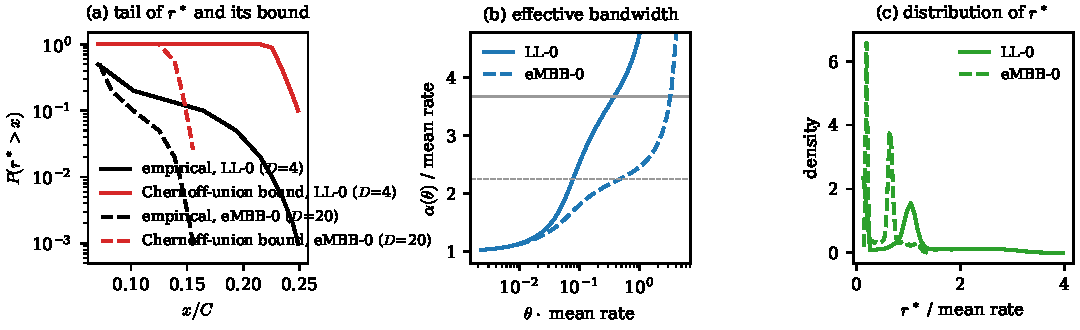
\includegraphics[width=\columnwidth]{paper_fig_theory}
\caption{Family M, load 0.80. (a) Empirical tail of $\rstar$ (black) and the Chernoff-union bound (red) for an LL cell ($D = 4$, solid) and an eMBB cell ($D = 20$, dashed). (b) Effective bandwidth $\alpha(\theta)$ relative to the mean rate; grey lines mark the peak phase rate. (c) Distribution of $\rstar$ relative to the mean rate.}
\label{fig:theory}
\end{figure}

\section{Controllers}
\label{sec:controllers}
\subsection{The learned-quantile KKT rule}
\label{sec:kkt}
The proposed rule of \cite{ncc2027} forecasts quantiles $q_i(\alpha_k)$ of $\rstar_i$ at levels $0.05, 0.25, 0.5, 0.75, 0.9, 0.95$ with one histogram gradient-boosted tree per quantile (pinball loss, 300 trees, 28 causal features: demand lags, exponentially weighted means, the last horizon's $\rstar$ and mean, the recent 90th percentile of $\rstar$, queue, head-of-line age, spectral efficiency and trend, cell one-hot; targets normalised by the cell peak). With $X_i \sim F_i$ the forecast and $w_i = w_i^{\rm p}$, it maximises $\sum_i w_i\E[\min(B_i + X_i, r_i)]$ subject to \eqref{eq:feasible}. Since $\partial_{r_i}\E[\min(B_i + X_i, r_i)] = 1 - F_i(r_i - B_i)$, the KKT conditions give
\begin{equation}
r_i(\lambda) = \mathrm{clip}\big(B_i + F_i^{-1}(1 - \lambda/w_i),\ 0,\ \mathrm{cap}_i\big),
\label{eq:kkt}
\end{equation}
with $\lambda^\ast$ found by bisection so that $\sum_i r_i = C$ (surplus, if any, is shared as headroom as in every baseline). The rule is feasible, cuts every cell at the same priority-weighted tail probability, funds observed backlog before uncertain demand, and loses at most $2\epsilon w_{\max}C$ of objective under a forecast with Kolmogorov error $\epsilon$ \cite{ncc2027}.

\subsection{Model-based predictive distributions}
Three controllers keep \eqref{eq:kkt} and replace the learned $F_i$ by a Markov-fluid model.
\textbf{Markov-chain KKT} (\emph{markov\_kkt}) quantises the last $W$ slots of each cell's demand into $K$ phases at fixed empirical quantiles, estimates $P$ with a Dirichlet prior, the phase means and coefficients of variation, and the current phase, then obtains the quantiles of $\rstar$ over the coming $H$ slots by Monte Carlo (200 paths) from the current phase. It needs no training data and is the natural model-based competitor. \textbf{Bound KKT} (\emph{eb\_kkt}) uses the same fitted chain but takes the quantiles from the Chernoff-union bound $U$ of Proposition~\ref{prop:union} under the stationary law; it is the controller that a reservation based on effective bandwidths would give. \textbf{True-model KKT} (\emph{markov\_oracle\_kkt}, Family M only) uses the generating chain of every cell, a hidden-Markov forward filter with Gamma emissions over the last 300 slots to obtain the posterior of the current phase, and Monte Carlo from that posterior. It is the best any model-based forecaster could do on Family M and is reported as a reference, not as an implementable controller.

\subsection{Predictive MaxWeight}
Plain MaxWeight allocates in decreasing order of $w_i^{\rm p}Q_i$ (plus a tuned head-of-line-age term) up to an EWMA usable-rate cap. Predictive MaxWeight \cite{huang2016} replaces the queue by the predicted queue $Q_i + \ell H\hat m_i$, where $\hat m_i$ is the forecast median of $\rstar_i$ from the same forecaster the proposed rule uses and $\ell$ a tuned look-ahead weight, and caps each cell's share at $Q_i/T + (1 + \mathrm{margin})\hat m_i$. It uses no deadlines and only one number of the forecast distribution. Tuned values: Family S margin and look-ahead \xpmwParamsS{}; Family G \xpmwParamsG{}; Family M \xpmwParamsM{}.

\subsection{Policy search}
The \emph{cem\_policy} controller reserves $B_i + F_i^{-1}(p_{\rm class(i)})$ with the learned forecaster and shares a shortage by weighted water-filling with a learned LL weight $w_{\rm LL}$. Its three parameters $(p_{\rm LL}, p_{\rm eMBB}, \log w_{\rm LL})$ are learned by the cross-entropy method \cite{rubinstein1999} on training seeds against the simulator (8 iterations, population 16, elite 4, smoothed mean update), i.e.\ from reward alone, as a DRL xApp would but with a parametrisation small enough to be learned reliably from about a hundred episodes. Learned values: Family S \xcemS{}; Family G \xcemG{}; Family M \xcemM{}.

\subsection{Variants of the proposed rule}
\label{sec:variants}
Three variants test the suggestions of Proposition~\ref{prop:sandwich} and property (c) of Sec.~\ref{sec:demand}. \emph{Volume-corrected weights} (\emph{proposed\_vc}) multiply $w_i$ by $\min(D_i + \hat l^\ast_i, T)$ with $\hat l^\ast_i$ the mean critical-window length of the last 30 horizons. \emph{Tuned LL weight} (\emph{proposed\_tw}) keeps \eqref{eq:kkt} unchanged but replaces the operator priority of the 2-ms class inside the rule by one scalar $w_{\rm LL}^{\rm rule} \in \{0.75, 1, 1.5, 2, 3, 4\}$ chosen on validation seeds; the metric still uses the operator priority. It separates the question ``is the KKT structure right'' from ``is the operator weight the right newsvendor weight''. \emph{Sustainable targets} retrain the forecaster on $\max(\rstar, \bar a)$ instead of $\rstar$ so that budgets also drain the interval's volume. Online conformal calibration (ACI \cite{gibbs2021}) and the window-quantile and transferred-forecaster ablations of \cite{ncc2027} are kept. Selected $w_{\rm LL}^{\rm rule}$: Family S \xtwS{}, Family G \xtwG{}, Family M \xtwM{}.

Table~\ref{tab:controllers} lists all controllers. Every one redistributes unused capacity as headroom; every tunable parameter is chosen on the validation seeds of its own family.

\begin{table}[t]
\caption{Compared controllers. WF: water-filling. The last three use the future or the generator and are references.}
\label{tab:controllers}
\centering
\scriptsize
\setlength{\tabcolsep}{3pt}
\begin{tabular}{lll}
\hline
Controller & Need estimate / allocation & Approximation \\
\hline
Static equal share & $C/N$ each & none \\
Reactive proportional & backlog/$T$ + EWMA; WF, unit $w$ & reactive \\
MaxWeight \cite{neely2010} & fill by $w^{\rm p}_iQ_i$ (+ HOL age) & drift \\
Predictive MaxWeight \cite{huang2016} & fill by $w^{\rm p}_i(Q_i + \ell H\hat m_i)$ & drift + forecast \\
Deadline-aware reactive & $B_i$ + last $\rstar$; WF, $w_i$ & reactive \\
Point forecast + WF & $B_i$ + median; WF, $w_i$ & one-step, point \\
Fixed quantile + WF & $B_i + F_i^{-1}(q)$, one $q$; WF & one-step, quantile \\
Policy search (CEM) & $B_i + F_i^{-1}(p_{\rm class})$; WF, learned $w$ & policy search \\
Bound q. + KKT & \eqref{eq:kkt}, quantiles of $U$ & one-step, bound \\
Markov MC q. + KKT & \eqref{eq:kkt}, fitted chain, MC & one-step, model \\
Proposed, window q. & \eqref{eq:kkt}, empirical quantiles & one-step, empirical \\
Proposed (GBM + KKT) & \eqref{eq:kkt}, learned quantiles & one-step, learned \\
Proposed, volume w. & \eqref{eq:kkt}, $w_i\min(D_i + \hat l^\ast_i, T)$ & one-step, learned \\
Proposed, tuned LL w. & \eqref{eq:kkt}, tuned $w^{\rm rule}_{\rm LL}$ & one-step, learned \\
Proposed + ACI & \eqref{eq:kkt}, per-cell level offsets & one-step, learned \\
Proposed, transferred & \eqref{eq:kkt}, other family's model & one-step, learned \\
True Markov model + KKT & \eqref{eq:kkt}, generator + HMM filter & reference (M) \\
Oracle water-fill & $B_i$ + true $\rstar$; WF, $w_i$ & reference \\
Oracle + KKT & $B_i$ + true $\rstar$; priority fill & reference \\
\hline
\end{tabular}
\end{table}

\section{Evaluation Methodology}
\label{sec:eval}
\subsection{Traffic families}
\label{sec:families}
No public per-slot, per-cell fronthaul traces exist (ColO-RAN \cite{colo_ran} reports KPIs at 250-ms resolution), so traffic is simulated with three independent families, each with its own forecaster and its own tuning.

\textbf{Family S} (synthetic, bursty): per cell, user bits are a Gamma smooth component plus heavy-tailed ON/OFF bursts with Pareto sojourns \cite{willinger1997}, modulated by piecewise-constant load regimes (mean 1~s) and converted to fronthaul bits with a slowly drifting spectral efficiency. Scenarios: low (0.50), moderate (0.65), high (0.80), flash crowds (0.80 with load multiplied by 1.8 for about 15\,\% of the time) and shift (0.80 with bursts 1.5 times stronger and longer and a heavier tail than anything seen in training or tuning).

\textbf{Family G} (standards-based): users dropped in a 3GPP TR~38.901 urban-macro cell (ISD 500~m, 3.5~GHz, 100~MHz) with six interfering sites, Rayleigh fading at 3~km/h mapped to the TS~38.214 CQI table, FTP Model~3 traffic on eMBB cells and XR video (60~fps, 30~Mbit/s) on LL cells, a round-robin PRB scheduler, and fronthaul demand equal to scheduled PRB-layers times $\beta$ \cite{tr38901,ts38214,tr36814,tr38838}. Loads 0.65 and 0.80.

\textbf{Family M} (Markov-modulated fluid, new): each cell is a three-phase (idle/normal/burst) Markov-modulated Gamma source with the structure of Sec.~\ref{sec:theory}. LL cells have mean sojourns of 40/30/8 slots and relative phase rates 0.15/1.0/3.0 with coefficients of variation 0.5/0.4/0.35; eMBB cells have sojourns 80/60/20 slots, rates 0.3/1.0/1.8 and coefficients 0.4/0.3/0.3; the phase-jump matrix is idle$\to$normal with probability 0.85, normal$\to$idle or burst with probability 0.5 each, burst$\to$normal with probability 0.85. Means are scaled so that the stationary offered load equals the target and the burst phase stays below the cell's air-interface peak. Scenarios: moderate (0.65), high (0.80) and \emph{shift} (0.80), in which the geometric sojourns are replaced by Pareto sojourns with index 1.5 and the same means, so the process is semi-Markov and every Markov model is misspecified. Realised loads: \xloadmmmoderate{}, \xloadmmhigh{}, \xloadmmshift{}.

\subsection{Protocol}
Training seeds (1000--1015, loads 0.5--0.95), validation seeds (2000--2003) and test seeds (3000--3019) are disjoint. One forecaster per family is trained once and frozen (Family S \xnTrainRowsS{} rows, Family G \xnTrainRowsG{}, Family M \xnTrainRowsM{}). Every tunable parameter of every controller, including the margins and look-ahead of the MaxWeight variants and the phase count and window of the Markov controllers, is chosen on the validation seeds (moderate and high scenarios) of its own family; the CEM policy is learned on training seeds. Each test run simulates 20\,000 slots (10~s) after a 1000-slot warm-up, every controller seeing the identical trace and the identical stale observations. We report means over \xnSeedsS{} seeds per scenario, and for paired comparisons the mean relative change with a 95\,\% percentile-bootstrap interval, the number of seeds won, and a two-sided Wilcoxon signed-rank test Holm-corrected across the comparisons of a scenario. In total the main comparison comprises \xnRunsS{} runs on Family S, \xnRunsG{} on Family G and \xnRunsM{} on Family M.

\section{Results}
\label{sec:results}

\begin{figure*}[t]
\centering
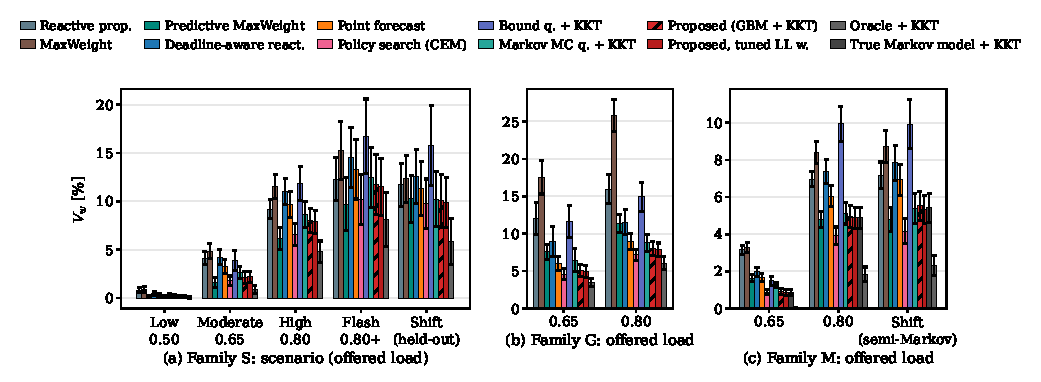
\includegraphics[width=0.95\textwidth]{paper_fig_overview_ext}
\caption{Priority-weighted deadline-violation ratio $V_w$ (mean $\pm$ std over \xnSeedsS{} test seeds; lower is better) of the main implementable controllers and the references on (a) Family S, (b) Family G and (c) Family M. Hatched: the closed-form learned-quantile KKT rule of the conference version.}
\label{fig:overview}
\end{figure*}

\subsection{Forecast quality}
Table~\ref{tab:forecast} compares the predictive distributions on the validation seeds of every family: the learned GBM, the empirical window quantiles, the fitted Markov chain and, on Family M, the true model with the hidden-phase filter. The learned forecaster has the lowest pinball loss of the implementable forecasters in every family; on Family M the fitted chain comes close and the true model is better still, as it must be. The fitted chain conditions on a quantised phase rather than on the sample path and is therefore less sharp; the window quantiles are the least sharp. This ordering is reproduced in the control results below, with one qualification that runs through the rest of the section: a sharper distribution helps a rule only as much as the rule's objective is aligned with the metric.

\begin{table}[t]
\caption{Forecast quality on validation seeds (deadline-feasible rate normalised by the cell peak; pinball loss averaged over the six levels)}
\label{tab:forecast}
\centering
\scriptsize
\setlength{\tabcolsep}{3pt}
\resizebox{\columnwidth}{!}{% ---- inlined from generated/tab_forecast ----
\begin{tabular}{llcccc}
\hline
Family & Forecaster & pinball$\times$100 & cov. 5/50/95 & 90\,\% PI cov. & med. rel. err. (\%) \\
\hline
S & GBM (learned) & 2.32 & 5/50/95 & 90 & 37 \\
 & window quantiles & 3.09 & 9/50/91 & 82 & 49 \\
 & fitted Markov chain & 3.26 & 25/56/84 & 59 & 48 \\
\hline
G & GBM (learned) & 2.97 & 34/56/98 & 98 & 24 \\
 & window quantiles & 4.22 & 38/60/94 & 90 & 60 \\
 & fitted Markov chain & 3.03 & 37/53/91 & 54 & 33 \\
\hline
M & GBM (learned) & 1.98 & 6/52/95 & 89 & 30 \\
 & window quantiles & 2.96 & 9/49/91 & 82 & 49 \\
 & fitted Markov chain & 2.94 & 25/54/86 & 62 & 45 \\
 & true Markov model & 1.89 & 6/50/95 & 89 & 28 \\
\hline
\end{tabular}
% ---- end generated/tab_forecast ----
}
\end{table}

\subsection{Three families, nineteen controllers}
\label{sec:res_main}
Tables~\ref{tab:main_S}--\ref{tab:main_M} and Fig.~\ref{fig:overview} report $V_w$ for every controller on the ten scenarios; Table~\ref{tab:h2h} places the closed-form rule next to its three strongest new competitors on each of them, with paired statistics. Four findings.

\textbf{(1) The conference result holds within its comparison set.} Against the twelve controllers of \cite{ncc2027} the learned-quantile KKT rule is still the best in all ten scenarios, including the two new Family M loads and the semi-Markov shift (\xmeanmmhighproposed{}\,\% against \xmeanmmhighpointforecast{}\,\% for the point forecast and \xmeanmmhighqueueaware{}\,\% for the deadline-aware reactive controller at load 0.80; \xmeanmmshiftproposed{}\,\% under shift). It is also the best controller that has no tuned parameter.

\textbf{(2) A reward-tuned policy with the same forecaster beats it.} The CEM policy, three parameters learned on training seeds, is the best implementable controller in \xwinscempolicy{} of the ten scenarios: both Family G loads (\xmeantgpphighcempolicy{}\,\% against \xmeantgpphighproposed{}\,\% at 0.80, paired change \xredtgpphighcempolicy{}\,\%, \xredtgpphighcempolicyWins{} seeds won by the KKT rule), all three Family M scenarios (\xmeanmmhighcempolicy{}\,\% against \xmeanmmhighproposed{}\,\% at 0.80; \xmeanmmshiftcempolicy{}\,\% against \xmeanmmshiftproposed{}\,\% under shift) and the low-load and shift scenarios of Family S. What it learned is the same in every family: an LL level of \xcemS{} in Family S, \xcemG{} in Family G and \xcemM{} in Family M, i.e.\ the 2-ms class is reserved at about the 80th percentile rather than at the higher percentile the equal-weighted-risk condition assigns it at $w_{\rm LL} = 3$, the eMBB class near its median, and a shortage shared with an LL weight close to one instead of three. The per-class ratios show the trade: at Family G load 0.80 the policy loses \xmeantgpphighcempolicyLL{}\,\% of LL bits against \xmeantgpphighproposedLL{}\,\% for the KKT rule and \xmeantgpphighcempolicyEMBB{}\,\% of eMBB bits against \xmeantgpphighproposedEMBB{}\,\%; weighted by three to one the eMBB saving is larger. This is the correction of Proposition~\ref{prop:sandwich}: a unit of LL rate shortfall costs $l^\ast + D \approx 7$ slots of volume and a unit of eMBB shortfall up to $T = 20$, so the newsvendor weight that minimises lost weighted bits is closer to one than to three.

The obvious test of this diagnosis is to change the weight inside the closed-form rule and nothing else, and it fails in an instructive way. The tuned-weight variant, with a single validation-chosen scalar on the LL weight (\xtwS{}, \xtwG{} and \xtwM{} in the three families), reaches \xmeanhighproposedtw{}\,\% at Family S high load, \xmeantgpphighproposedtw{}\,\% at Family G high load and \xmeanmmhighproposedtw{}\,\% at Family M high load against \xmeanhighproposed{}, \xmeantgpphighproposed{} and \xmeanmmhighproposed{}\,\% for the plain rule: paired changes of \xredhighproposedtw{}, \xredtgpphighproposedtw{} and \xredmmhighproposedtw{}\,\%, significant but one order of magnitude smaller than the distance to the CEM policy (\xmeanhighcempolicy{}, \xmeantgpphighcempolicy{} and \xmeanmmhighcempolicy{}\,\%). Its only win is the moderate load of Family M (\xmeanmmmoderateproposedtw{}\,\% against \xmeanmmmoderatecempolicy{}\,\% for the CEM policy), and the validation surface is flat enough that Family M selects $w^{\rm rule}_{\rm LL} = 4$, the opposite direction. The reason is in the structure of \eqref{eq:kkt}. On the high-load scenarios the capacity constraint binds in \xlamBindS{}\,\% (S), \xlamBindG{}\,\% (G) and \xlamBindM{}\,\% (M) of the intervals, and in \xlamFloorS{}, \xlamFloorG{} and \xlamFloorM{}\,\% of them the common multiplier $\lambda^\ast$ reaches the eMBB weight, so every eMBB cell is already at its lowest quantile plus its proportional share of the slack and the LL cells sit near the \xlamLLlevelS{}th (S), \xlamLLlevelG{}th (G) and \xlamLLlevelM{}th (M) percentile. Lowering the LL weight moves the LL cells along a quantile curve that is flat at these levels and returns the freed rate to the eMBB cells through the same proportional slack rule, which does not know which eMBB cell will burst; the CEM policy instead holds the eMBB level at a fixed median-like quantile for every cell (\xcemS{}, \xcemG{}, \xcemM{}) and shares only the residual shortage, which is a different mapping from forecast to budget and not a different constant in the same mapping. The equal-weighted-risk structure, the feasibility and backlog-first properties and the closed form are intact; what is missing is a per-class level that does not collapse when $\lambda^\ast$ saturates.

\textbf{(3) Predictive back-pressure wins where bursts are short.} Predictive MaxWeight, which uses the forecast median and the queues and no deadline model, is the best implementable controller in the moderate, high and flash-crowd scenarios of Family S (\xmeanhighpredmaxweight{}\,\% against \xmeanhighproposed{}\,\% for the KKT rule and \xmeanhighcempolicy{}\,\% for the CEM policy at high load; paired change \xredhighpredmaxweight{}\,\% against the KKT rule, \xredhighpredmaxweightWins{} seeds), is second in Family M (\xmeanmmhighpredmaxweight{}\,\% at 0.80), and is poor in Family G (\xmeantgpphighpredmaxweight{}\,\%, worse than the point-forecast water-fill), where periodic XR frames queue behind FTP files once the cap is a volume rather than a peak. The LL bursts of Family S last a few slots; a reservation at the 2-ms peak rate, held for 10~ms, idles for most of the interval (\xmeanhighproposedUnused{}\,\% of the allocated capacity goes unused under the KKT rule against \xmeanhighpredmaxweightUnused{}\,\% under predictive MaxWeight), and a queue weight that includes the predicted volume is a better guide to who needs the link than a deadline-feasible peak. Sec.~\ref{sec:regime} shows that this is a property of the interval, not of the family.

\textbf{(4) Model-based distributions are a credible substitute, bounds are not.} The KKT rule driven by a Markov chain fitted online, with no training data at all, is within \xredmmhighmarkovkkt{}\,\% of the learned rule on Family M at load 0.80 (where the model is correct) and \xredtgpphighmarkovkkt{}\,\% on Family G; under the semi-Markov shift, where every Markov model is misspecified, it reaches \xmeanmmshiftmarkovkkt{}\,\% against \xmeanmmshiftproposed{}\,\% for the learned rule, so three phases fitted to the last 0.5--1.5~s carry most of the usable information even when the sojourn law is wrong. The true-model reference with the hidden-phase filter gives \xmeanmmhighmarkovoraclekkt{}\,\% at load 0.80; the distance from the learned rule to it (\xgapMarkovOraclemmhigh{}\,\% of the former) is the price of learning the distribution from features instead of knowing the generator, and the distance from it to the oracle + KKT rule (\xmeanmmhighoraclekkt{}\,\%) is the irreducible uncertainty of the phase process over 22 slots. The rule driven by the Chernoff-union bound is the worst deadline-aware controller everywhere (\xmeanhighebkkt{}\,\% in Family S, \xmeanmmhighebkkt{}\,\% in Family M at high load), because it reserves the quantiles of a bound that Sec.~\ref{sec:theory_num} showed to be 25--100 times conservative and starves the eMBB class (\xmeanmmhighebkktEMBB{}\,\% eMBB loss).

\begin{table*}[t]
\caption{Family S: $V_w$ (\%, mean $\pm$ std over \xnSeedsS{} test seeds; lower is better). Last column: paired change of $V_w$ relative to the learned-quantile KKT rule at high load (\%; negative means the row is better; seeds won by the KKT rule out of \xnSeedsS{}; $^{\ast}$/$^{\ast\ast}$: Holm-corrected $p < 0.05$/$0.01$).}
\label{tab:main_S}
\centering
\footnotesize
\setlength{\tabcolsep}{3pt}
% ---- inlined from generated/tab_main_S ----
\begin{tabular}{lcccccc}
\hline
Controller & Low 0.50 & Mod. 0.65 & High 0.80 & Flash & Shift & $\Delta$ (wins) \\
\hline
Static equal share & 4.45$\pm$1.05 & 9.65$\pm$1.36 & 15.46$\pm$1.51 & 19.15$\pm$2.34 & 22.31$\pm$2.99 & -48 (20)$^{\ast\ast}$ \\
Reactive proportional & 0.83$\pm$0.27 & 4.11$\pm$0.69 & 9.20$\pm$0.99 & 12.27$\pm$2.23 & 11.70$\pm$2.24 & -13 (20)$^{\ast\ast}$ \\
MaxWeight (drift) & 0.90$\pm$0.28 & 4.85$\pm$0.79 & 11.54$\pm$1.27 & 15.24$\pm$3.02 & 12.31$\pm$2.44 & -31 (20)$^{\ast\ast}$ \\
Predictive MaxWeight & 0.14$\pm$0.10 & 1.62$\pm$0.51 & 6.15$\pm$1.13 & 9.69$\pm$2.73 & 10.25$\pm$2.42 & +30 (0)$^{\ast\ast}$ \\
Deadline-aware react. & 0.52$\pm$0.21 & 4.24$\pm$0.78 & 11.03$\pm$1.33 & 14.51$\pm$3.06 & 12.56$\pm$2.81 & -27 (20)$^{\ast\ast}$ \\
Point forecast + WF & 0.27$\pm$0.17 & 3.23$\pm$0.73 & 9.70$\pm$1.34 & 13.33$\pm$3.09 & 11.30$\pm$2.81 & -18 (20)$^{\ast\ast}$ \\
Fixed quantile + WF & 0.34$\pm$0.23 & 4.35$\pm$1.02 & 11.76$\pm$1.44 & 15.09$\pm$3.17 & 12.85$\pm$3.32 & -32 (20)$^{\ast\ast}$ \\
Policy search (CEM) & 0.13$\pm$0.10 & 1.77$\pm$0.51 & 6.57$\pm$1.15 & 10.20$\pm$2.57 & 9.73$\pm$2.58 & +22 (0)$^{\ast\ast}$ \\
Bound quantiles + KKT & 0.29$\pm$0.19 & 3.88$\pm$1.03 & 11.85$\pm$1.74 & 16.71$\pm$3.86 & 15.79$\pm$4.14 & -33 (20)$^{\ast\ast}$ \\
Markov MC quantiles + KKT & 0.25$\pm$0.13 & 2.65$\pm$0.65 & 8.64$\pm$1.31 & 12.44$\pm$3.10 & 10.22$\pm$2.84 & -7 (20)$^{\ast\ast}$ \\
Proposed, window q. & 0.25$\pm$0.13 & 2.57$\pm$0.64 & 8.72$\pm$1.34 & 12.67$\pm$3.19 & 10.22$\pm$2.88 & -8 (20)$^{\ast\ast}$ \\
Proposed (GBM + KKT) & 0.15$\pm$0.13 & 2.15$\pm$0.60 & 8.00$\pm$1.27 & 11.76$\pm$3.08 & 10.04$\pm$2.71 & -- \\
Proposed, volume weights & 0.18$\pm$0.13 & 2.21$\pm$0.57 & 7.89$\pm$1.18 & 11.51$\pm$2.95 & 9.95$\pm$2.66 & +1 (4)$^{\ast\ast}$ \\
Proposed, tuned LL weight & 0.18$\pm$0.13 & 2.21$\pm$0.57 & 7.88$\pm$1.18 & 11.49$\pm$2.95 & 9.90$\pm$2.59 & +1 (4)$^{\ast\ast}$ \\
Proposed + ACI & 0.17$\pm$0.13 & 2.17$\pm$0.61 & 8.14$\pm$1.30 & 12.27$\pm$3.26 & 11.12$\pm$3.22 & -2 (19)$^{\ast\ast}$ \\
\hline
Oracle water-fill & 0.07$\pm$0.10 & 1.62$\pm$0.56 & 6.89$\pm$1.28 & 10.16$\pm$2.96 & 6.69$\pm$2.60 & +16 (0)$^{\ast\ast}$ \\
Oracle + KKT rule & 0.05$\pm$0.09 & 0.88$\pm$0.42 & 4.77$\pm$1.12 & 8.10$\pm$2.77 & 5.84$\pm$2.37 & +68 (0)$^{\ast\ast}$ \\
\hline
\end{tabular}
% ---- end generated/tab_main_S ----

\end{table*}

\begin{table*}[t]
\caption{Family G: $V_w$ (\%, mean $\pm$ std over \xnSeedsG{} test seeds) and paired change relative to the learned-quantile KKT rule at load 0.80.}
\label{tab:main_G}
\centering
\footnotesize
\setlength{\tabcolsep}{3pt}
% ---- inlined from generated/tab_main_G ----
\begin{tabular}{lccc}
\hline
Controller & Mod. 0.65 & High 0.80 & $\Delta$ (wins) \\
\hline
Static equal share & 10.75$\pm$1.71 & 13.10$\pm$2.13 & -39 (20)$^{\ast\ast}$ \\
Reactive proportional & 12.05$\pm$2.18 & 15.94$\pm$1.93 & -50 (20)$^{\ast\ast}$ \\
MaxWeight (drift) & 17.51$\pm$2.21 & 25.79$\pm$2.15 & -69 (20)$^{\ast\ast}$ \\
Predictive MaxWeight & 7.57$\pm$0.99 & 11.36$\pm$1.19 & -29 (20)$^{\ast\ast}$ \\
Deadline-aware react. & 8.95$\pm$2.04 & 11.53$\pm$1.67 & -31 (20)$^{\ast\ast}$ \\
Point forecast + WF & 6.00$\pm$0.94 & 8.98$\pm$1.09 & -11 (20)$^{\ast\ast}$ \\
Fixed quantile + WF & 6.80$\pm$1.15 & 9.88$\pm$1.24 & -19 (20)$^{\ast\ast}$ \\
Policy search (CEM) & 4.58$\pm$0.71 & 7.17$\pm$0.75 & +12 (0)$^{\ast\ast}$ \\
Bound quantiles + KKT & 11.68$\pm$2.14 & 14.91$\pm$1.94 & -46 (20)$^{\ast\ast}$ \\
Markov MC quantiles + KKT & 6.44$\pm$1.54 & 8.77$\pm$1.11 & -9 (20)$^{\ast\ast}$ \\
Proposed, window q. & 6.18$\pm$0.99 & 9.01$\pm$1.04 & -11 (20)$^{\ast\ast}$ \\
Proposed (GBM + KKT) & 5.08$\pm$0.84 & 8.01$\pm$0.99 & -- \\
Proposed, volume weights & 11.76$\pm$1.19 & 18.30$\pm$1.55 & -56 (20)$^{\ast\ast}$ \\
Proposed, tuned LL weight & 4.98$\pm$0.79 & 7.83$\pm$0.93 & +2 (0)$^{\ast\ast}$ \\
Proposed + ACI & 5.41$\pm$0.87 & 8.27$\pm$0.98 & -3 (19)$^{\ast\ast}$ \\
Proposed, transferred & 6.99$\pm$1.29 & 9.89$\pm$1.18 & -19 (20)$^{\ast\ast}$ \\
Oracle water-fill & 4.82$\pm$0.76 & 7.85$\pm$1.06 & +2 (5)$^{\ast}$ \\
Oracle + KKT rule & 3.47$\pm$0.57 & 6.06$\pm$0.83 & +32 (0)$^{\ast\ast}$ \\
\hline
\end{tabular}
% ---- end generated/tab_main_G ----

\end{table*}

\begin{table*}[t]
\caption{Family M: $V_w$ (\%, mean $\pm$ std over \xnSeedsM{} test seeds) and paired change relative to the learned-quantile KKT rule at load 0.80. The true-model controller knows the generating chain and is a reference.}
\label{tab:main_M}
\centering
\footnotesize
\setlength{\tabcolsep}{3pt}
% ---- inlined from generated/tab_main_M ----
\begin{tabular}{lcccc}
\hline
Controller & Mod. 0.65 & High 0.80 & Shift 0.80 & $\Delta$ (wins) \\
\hline
Static equal share & 4.88$\pm$0.37 & 12.15$\pm$0.59 & 11.62$\pm$0.75 & -59 (20)$^{\ast\ast}$ \\
Reactive proportional & 3.17$\pm$0.24 & 6.97$\pm$0.41 & 7.17$\pm$0.72 & -29 (20)$^{\ast\ast}$ \\
MaxWeight (drift) & 3.29$\pm$0.27 & 8.40$\pm$0.60 & 8.73$\pm$0.86 & -41 (20)$^{\ast\ast}$ \\
Predictive MaxWeight & 1.64$\pm$0.17 & 4.79$\pm$0.42 & 4.80$\pm$0.63 & +3 (8)$^{\ast}$ \\
Deadline-aware react. & 1.98$\pm$0.25 & 7.37$\pm$0.64 & 7.84$\pm$0.95 & -33 (20)$^{\ast\ast}$ \\
Point forecast + WF & 1.68$\pm$0.20 & 6.04$\pm$0.56 & 6.92$\pm$0.85 & -18 (20)$^{\ast\ast}$ \\
Fixed quantile + WF & 1.43$\pm$0.18 & 6.52$\pm$0.64 & 6.73$\pm$0.75 & -24 (20)$^{\ast\ast}$ \\
Policy search (CEM) & 0.88$\pm$0.13 & 3.93$\pm$0.46 & 4.17$\pm$0.65 & +26 (0)$^{\ast\ast}$ \\
Bound quantiles + KKT & 1.48$\pm$0.24 & 9.94$\pm$0.94 & 9.92$\pm$1.33 & -50 (20)$^{\ast\ast}$ \\
Markov MC quantiles + KKT & 1.24$\pm$0.13 & 5.12$\pm$0.57 & 5.39$\pm$0.80 & -3 (19)$^{\ast\ast}$ \\
Proposed, window q. & 1.26$\pm$0.13 & 5.40$\pm$0.60 & 5.65$\pm$0.89 & -8 (20)$^{\ast\ast}$ \\
Proposed (GBM + KKT) & 0.92$\pm$0.17 & 4.94$\pm$0.58 & 5.52$\pm$0.77 & -- \\
Proposed, volume weights & 0.97$\pm$0.17 & 5.02$\pm$0.56 & 5.82$\pm$0.78 & -2 (17)$^{\ast\ast}$ \\
Proposed, tuned LL weight & 0.85$\pm$0.17 & 4.88$\pm$0.58 & 5.31$\pm$0.76 & +1 (4)$^{\ast\ast}$ \\
Proposed + ACI & 0.97$\pm$0.17 & 4.97$\pm$0.58 & 5.66$\pm$1.01 & -1 (11) \\
Proposed, transferred & 1.59$\pm$0.15 & 5.54$\pm$0.56 & 5.27$\pm$0.83 & -11 (20)$^{\ast\ast}$ \\
True Markov model + KKT & 0.88$\pm$0.16 & 4.89$\pm$0.56 & 5.42$\pm$0.77 & +1 (6)$^{\ast\ast}$ \\
Oracle water-fill & 0.07$\pm$0.04 & 2.49$\pm$0.44 & 3.05$\pm$0.57 & +99 (0)$^{\ast\ast}$ \\
Oracle + KKT rule & 0.03$\pm$0.03 & 1.84$\pm$0.39 & 2.31$\pm$0.55 & +168 (0)$^{\ast\ast}$ \\
\hline
\end{tabular}
% ---- end generated/tab_main_M ----

\end{table*}

\begin{table*}[t]
\caption{The learned-quantile KKT rule against its three strongest new competitors on every scenario ($V_w$ in \%; $\Delta$ = paired change relative to the KKT rule, negative means the competitor is better; wins = seeds won by the KKT rule; $^{\ast}$/$^{\ast\ast}$: Holm-corrected $p<0.05$/$0.01$; last column: best implementable controller of all nineteen)}
\label{tab:h2h}
\centering
\scriptsize
\setlength{\tabcolsep}{3pt}
% ---- inlined from generated/tab_head_to_head ----
\begin{tabular}{lcccccccl}
\hline
Scenario & Proposed (GBM + KKT) & \multicolumn{2}{c}{Predictive MaxWeight} & \multicolumn{2}{c}{Policy search (CEM)} & \multicolumn{2}{c}{Markov MC quantiles + KKT} & best implementable \\
 & $V_w$ & $V_w$ & $\Delta$ [95\,\% CI], wins & $V_w$ & $\Delta$ [95\,\% CI], wins & $V_w$ & $\Delta$ [95\,\% CI], wins & \\
\hline
S Low 0.50 & 0.15 & 0.14 & +8 [-11, +31] 7/20 & 0.13 & +15 [+3, +31]$^{\ast}$ 6/20 & 0.25 & -39 [-49, -29]$^{\ast\ast}$ 20/20 & Policy search (CEM) \\
S Mod. 0.65 & 2.15 & 1.62 & +33 [+27, +39]$^{\ast\ast}$ 0/20 & 1.77 & +22 [+18, +25]$^{\ast\ast}$ 0/20 & 2.65 & -19 [-21, -17]$^{\ast\ast}$ 20/20 & Predictive MaxWeight \\
S High 0.80 & 8.00 & 6.15 & +30 [+27, +34]$^{\ast\ast}$ 0/20 & 6.57 & +22 [+20, +24]$^{\ast\ast}$ 0/20 & 8.64 & -7 [-8, -7]$^{\ast\ast}$ 20/20 & Predictive MaxWeight \\
S Flash & 11.76 & 9.69 & +21 [+20, +23]$^{\ast\ast}$ 0/20 & 10.20 & +15 [+13, +17]$^{\ast\ast}$ 0/20 & 12.44 & -6 [-6, -5]$^{\ast\ast}$ 20/20 & Predictive MaxWeight \\
S Shift & 10.04 & 10.25 & -2 [-4, 0]$^{\ast}$ 15/20 & 9.73 & +3 [+2, +4]$^{\ast\ast}$ 3/20 & 10.22 & -2 [-3, -1]$^{\ast\ast}$ 16/20 & Policy search (CEM) \\
G Mod. 0.65 & 5.08 & 7.57 & -33 [-36, -30]$^{\ast\ast}$ 20/20 & 4.58 & +11 [+9, +13]$^{\ast\ast}$ 0/20 & 6.44 & -21 [-25, -17]$^{\ast\ast}$ 20/20 & Policy search (CEM) \\
G High 0.80 & 8.01 & 11.36 & -29 [-32, -27]$^{\ast\ast}$ 20/20 & 7.17 & +12 [+10, +14]$^{\ast\ast}$ 0/20 & 8.77 & -9 [-10, -7]$^{\ast\ast}$ 20/20 & Policy search (CEM) \\
M Mod. 0.65 & 0.92 & 1.64 & -44 [-46, -41]$^{\ast\ast}$ 20/20 & 0.88 & +4 [+1, +7]$^{\ast\ast}$ 5/20 & 1.24 & -26 [-29, -23]$^{\ast\ast}$ 20/20 & Proposed, tuned LL weight \\
M High 0.80 & 4.94 & 4.79 & +3 [+1, +5]$^{\ast}$ 8/20 & 3.93 & +26 [+24, +27]$^{\ast\ast}$ 0/20 & 5.12 & -3 [-5, -2]$^{\ast\ast}$ 19/20 & Policy search (CEM) \\
M Shift 0.80 & 5.52 & 4.80 & +15 [+13, +17]$^{\ast\ast}$ 0/20 & 4.17 & +33 [+31, +35]$^{\ast\ast}$ 0/20 & 5.39 & +2 [+1, +4]$^{\ast\ast}$ 4/20 & Policy search (CEM) \\
\hline
\end{tabular}
% ---- end generated/tab_head_to_head ----

\end{table*}

\subsection{Reservation versus back-pressure: the operating regime}
\label{sec:regime}
Fig.~\ref{fig:regime} and Table~\ref{tab:sweep} vary the control interval $T$ and the telemetry delay $\tau$ on the high-load scenario of Family S with forecasters retrained per setting. The ordering between the reservation rules and predictive MaxWeight flips with $T$. At $T = 2$~ms, the LL deadline, the KKT rule gives \xsweepTfourproposed{}\,\% against \xsweepTfourpredmaxweight{}\,\% for predictive MaxWeight; at $T = 5$~ms \xsweepTonezeroproposed{}\,\% against \xsweepTonezeropredmaxweight{}\,\%; at $T = 10$~ms \xsweepTtwozeroproposed{}\,\% against \xsweepTtwozeropredmaxweight{}\,\%; at $T = 20$~ms, five times the LL deadline, \xsweepTfourzeroproposed{}\,\% against \xsweepTfourzeropredmaxweight{}\,\%. The crossover lies between 5 and 10~ms for Family S, whose LL bursts last a few slots. A deadline-aware reservation is the right structure when the interval is short enough that a reserved peak is used before the interval ends; back-pressure with a volume forecast is the right structure when the interval is long compared with the bursts, because the reservation then idles and the queue is the better guide. Family G sits on the reservation side at $T = 10$~ms because its bursts (FTP files, XR frames) are as long as the interval; Family M at load 0.80, with LL burst sojourns of 8 slots, sits near the crossover. Telemetry delay moves all controllers up together and does not change the ordering at $T = 10$~ms. With a perfect forecast the KKT rule beats predictive MaxWeight at every $T$ (oracle + KKT in Fig.~\ref{fig:regime}), so the loss of the implementable reservation at long intervals is forecast error compounded by commitment: the forecast quantile of a short burst is right about its height and wrong about its timing within the interval, and a reservation pays for the timing error whereas back-pressure does not. The tuned-weight rule and the CEM policy, which reserve the 2-ms class less aggressively, move the crossover to longer intervals but do not remove it.

\begin{figure}[t]
\centering
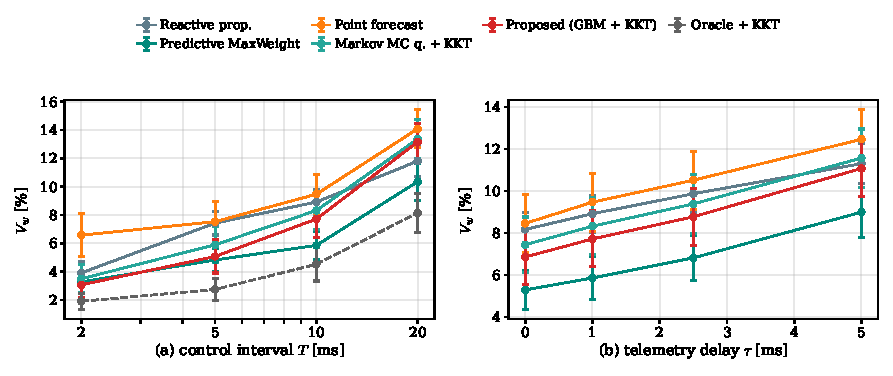
\includegraphics[width=\columnwidth]{paper_fig_regime}
\caption{Family S, high load: $V_w$ against (a) the control interval $T$ (forecasters retrained per $T$, \xnSeedsSweep{} seeds) and (b) the telemetry delay $\tau$. Reservation rules win at short intervals, predictive MaxWeight at long ones; with a perfect forecast (oracle + KKT, dashed) the reservation wins everywhere.}
\label{fig:regime}
\end{figure}

\begin{table}[t]
\caption{Family S, high load: $V_w$ (\%) against the control interval $T$ (\xnSeedsSweep{} seeds)}
\label{tab:sweep}
\centering
\scriptsize
% ---- inlined from generated/tab_sweep ----
\begin{tabular}{lcccc}
\hline
Controller $\backslash$ $T$ & 2 ms & 5 ms & 10 ms & 20 ms \\
\hline
Reactive proportional & 3.91 & 7.42 & 8.91 & 11.80 \\
Predictive MaxWeight & 3.27 & 4.82 & 5.85 & 10.35 \\
Deadline-aware react. & 7.89 & 10.20 & 10.78 & 15.84 \\
Point forecast + WF & 6.57 & 7.53 & 9.46 & 14.08 \\
Policy search (CEM) & 4.39 & 4.76 & 6.23 & 11.00 \\
Markov MC quantiles + KKT & 3.50 & 5.90 & 8.32 & 13.36 \\
Proposed (GBM + KKT) & 3.07 & 5.07 & 7.71 & 13.15 \\
Proposed, tuned LL weight & 2.82 & 4.76 & 7.57 & 13.05 \\
\hline
Oracle water-fill & 6.89 & 6.01 & 6.63 & 10.83 \\
Oracle + KKT rule & 1.91 & 2.74 & 4.52 & 8.14 \\
\hline
\end{tabular}
% ---- end generated/tab_sweep ----

\end{table}

\subsection{The objective and the priority weight across families}
\label{sec:weights}
Table~\ref{tab:weights} sweeps the operator weight $w^{\rm p}_{\rm LL}$ on the high-load scenario of every family, with all controllers told the new weight and parameters tuned at $w_{\rm LL} = 3$. In Family S predictive MaxWeight leads at every weight and the KKT rule's gap to it is largest at $w_{\rm LL} = 1$, where a deadline-aware reservation has nothing to trade. In Family G the KKT rule leads the conference comparison set from $w_{\rm LL} = 2$ on and the point-forecast water-fill is better at $w_{\rm LL} = 1$, as in \cite{ncc2027}; the CEM policy, whose learned LL weight is close to one, leads at every weight, and predictive MaxWeight does not catch up at any. In Family M the CEM policy leads, predictive MaxWeight and the KKT rule follow within a few percent of each other. The practical reading: a deadline-aware reservation is for operators who value a low-latency bit at least two to three times an eMBB bit \emph{and} whose control interval is short relative to their bursts; and whatever the operator weight, the newsvendor weight inside the rule should be tuned, not copied.

\begin{table*}[t]
\caption{Operator LL weight sweep at high load in the three families: $V_w$ (\%, \xnSeedsWeights{} seeds; parameters tuned at $w_{\rm LL} = 3$)}
\label{tab:weights}
\centering
\scriptsize
\setlength{\tabcolsep}{3pt}
% ---- inlined from generated/tab_weights ----
\begin{tabular}{l|cccc|cccc|cccc}
\hline
& \multicolumn{4}{c}{Family S, High 0.80} & \multicolumn{4}{c}{Family G, High 0.80} & \multicolumn{4}{c}{Family M, High 0.80} \\
Controller $\backslash$ $w_{\mathrm{LL}}$ & 1 & 2 & 3 & 5 & 1 & 2 & 3 & 5 & 1 & 2 & 3 & 5 \\
\hline
Reactive proportional & 6.55 & 8.13 & 9.20 & 10.56 & 15.01 & 15.62 & 15.94 & 16.27 & 3.48 & 5.56 & 6.97 & 8.77 \\
MaxWeight (drift) & 7.38 & 9.96 & 11.54 & 13.38 & 19.77 & 23.92 & 25.79 & 27.29 & 4.52 & 6.87 & 8.40 & 10.31 \\
Predictive MaxWeight & 5.88 & 6.43 & 6.15 & 5.62 & 18.44 & 16.69 & 11.36 & 7.41 & 2.84 & 4.04 & 4.79 & 5.75 \\
Deadline-aware react. & 7.75 & 10.08 & 11.03 & 11.69 & 13.19 & 12.50 & 11.53 & 9.99 & 3.20 & 5.66 & 7.37 & 9.32 \\
Point forecast + WF & 6.77 & 8.90 & 9.70 & 10.57 & 10.43 & 9.74 & 8.98 & 7.61 & 2.87 & 4.81 & 6.04 & 7.51 \\
Policy search (CEM) & 6.84 & 6.68 & 6.57 & 6.43 & 10.89 & 8.43 & 7.17 & 5.88 & 2.89 & 3.51 & 3.93 & 4.46 \\
Proposed (GBM + KKT) & 6.58 & 8.35 & 8.00 & 6.93 & 15.92 & 9.74 & 8.01 & 5.90 & 3.10 & 4.80 & 4.94 & 4.92 \\
Proposed, tuned LL weight & 9.05 & 8.35 & 7.88 & 7.28 & 13.49 & 9.74 & 7.83 & 5.88 & 4.87 & 4.88 & 4.88 & 4.88 \\
\hline
Oracle water-fill & 4.86 & 5.97 & 6.89 & 8.29 & 8.78 & 8.31 & 7.85 & 6.76 & 1.26 & 1.85 & 2.49 & 4.37 \\
Oracle + KKT rule & 4.86 & 5.68 & 4.77 & 3.63 & 8.78 & 7.78 & 6.06 & 4.31 & 1.26 & 2.19 & 1.84 & 1.40 \\
\hline
\end{tabular}
% ---- end generated/tab_weights ----

\end{table*}

\subsection{Negative results}
\label{sec:negative}
Four ideas suggested by the theory did not improve the closed-form rule, and we report them because they are the obvious next things a reader would try. \emph{Volume-corrected weights}, the literal implementation of the $l^\ast + D$ factor, give \xmeanhighproposedvc{}\,\% against \xmeanhighproposed{}\,\% at high load in Family S, a small gain, but \xmeantgpphighproposedvc{}\,\% in Family G: with zero-inflated XR and FTP demand the estimated critical windows of the LL cells are short and the correction removes nearly all of their protection (\xmeantgpphighproposedvcLL{}\,\% LL loss). A \emph{tuned scalar} on the LL weight (Sec.~\ref{sec:variants}) is safe but small, 1--2\,\% at high load, for the saturation reason given in Sec.~\ref{sec:res_main}; it is kept in the tables as the best the rule can do without changing its form. Two backlog-floor variants that give a cell with $p_i \le 0$ at least its backlog $B_i$ or $Q_i/T$ before the slack is shared were also tried: the $B_i$ floor starves the LL class (18\,\% LL loss in Family G) and the $Q_i/T$ floor is mixed, so neither is reported in the tables. \emph{Sustainable targets}, which forecast $\max(\rstar, \bar a)$ so that budgets also drain the volume, raise every LL reservation and degrade $V_w$ in both original families. \emph{Drift-weighted} KKT, which multiplies $w_i$ by a queue-dependent factor to blend the newsvendor rule with back-pressure, degrades as well: the newsvendor rule already funds backlog first, so a queue weight double-counts it. \emph{Bound quantiles} over-reserve by the factors of Table~\ref{tab:theory}, and \emph{per-stream conformal correction} (ACI) inflates LL reservations and starves eMBB, as in \cite{ncc2027}. Each of these is a one-line change in the released code.

\subsection{Compression, miscalibration and cost}
The BFP mantissa width (6, 9, 12, 14 bits) rescales $\beta$ and moves the offered load from 0.44 to 0.99 with the same user traffic; the conclusion of \cite{ncc2027} that deadline-aware allocation matters between loads of about 0.5 and 0.8 and that no rule helps above 0.9 holds for the new controllers as well (at 9 bits, load 0.65: \xcompBnineproposed{}\,\% for the KKT rule, \xcompBninepredmaxweight{}\,\% for predictive MaxWeight, \xcompBninecempolicy{}\,\% for the CEM policy; at 14 bits, load 0.99: \xcompBonefourproposed{}, \xcompBonefourpredmaxweight{} and \xcompBonefourcempolicy{}\,\%). The miscalibration sweep of \cite{ncc2027} (quantile levels shifted by $\epsilon \in [-0.3, 0.3]$) is unchanged. Decision times of the Python prototype per 10-ms epoch on a 4-core CPU: KKT rule \xdtproposed{}~ms (1800 trees), CEM policy \xdtcempolicy{}~ms, predictive MaxWeight \xdtpredmaxweight{}~ms, Markov-chain KKT \xdtmarkovkkt{}~ms (chain fit and 200 Monte Carlo paths per cell), true-model KKT \xdtmarkovoraclekkt{}~ms; compiled implementations of all but the last fit comfortably in a 10-ms loop.

\section{Discussion and Conclusion}
\label{sec:conclusion}
This article set out to double-check a result that looked too clean. The conference version showed that a learned predictive distribution of deadline-feasible demand, turned into budgets by a closed-form KKT rule, beats point forecasts, tuned global quantiles and reactive controllers. That remains true in all ten scenarios of three unrelated traffic families. But when the comparison set is widened to the other tractable approximations of the control problem, two controllers that use the same forecaster are better: a three-parameter policy whose levels and weight are learned from reward, in \xwinscempolicy{} scenarios, and a predictive back-pressure controller that uses only the forecast median, in \xwinspredmaxweight{}. The theory explains the direction of both and the measurements explain why the closed-form rule cannot follow. The newsvendor surrogate is a lower bound on the violated volume whose per-cell factor is the critical-window length plus the deadline (Proposition~\ref{prop:sandwich}), so a rule that uses the operator's weight as its newsvendor weight over-protects the short-deadline class; the learned policies correct this, but the same correction inside the KKT rule is worth only 1--4\,\% because the common multiplier saturates at the eMBB weight in half of the loaded intervals and the rule then has no per-class level left to move. And the tail of the deadline-feasible rate at millisecond deadlines is governed by the recent sample path, not by the stationary law (Sec.~\ref{sec:theory_num}), so a forecast can be right about the height of a burst and wrong about its timing; a reservation held for an interval longer than the burst pays for the timing error and back-pressure does not.

Design guidance follows. Use the closed-form rule with a learned or online-fitted distribution when no reward signal or digital twin is available; it is the best controller with nothing to tune and is never far from the best. When a twin exists, learn the per-class quantile levels and the sharing weight from reward with the same forecaster; three parameters and a few hundred episodes are enough, and a tuned weight alone is not. If the control interval can be set to the shortest deadline or a small multiple of it, the reservation is the best structure at every weight; if the interval is fixed at several times the shortest deadline, as in a 10-ms loop over 2-ms traffic, and the bursts are shorter than the interval, predictive MaxWeight is better; if the bursts are as long as the interval (file transfers, periodic frames), the reservation is. The Markov-fluid bounds are admission and dimensioning tools, not reservation rules, at these deadlines. A Markov chain fitted online is a usable substitute for the learned forecaster when no training data exist, even under semi-Markov sojourns.

Limitations remain those of the conference version: all three families are simulated; Family G uses a round-robin scheduler and a fixed rank; the link is a budget-enforced pipe without a switch-queue model; each cell carries one class; HARQ, uplink and the signal-quality cost of compression are not modelled. Three are specific to this article: the MDP of Sec.~\ref{sec:mdp} is approximated, not solved; the CEM policy is learned on the same training seeds as the forecaster, so its search saw slightly optimistic forecasts; and a stronger policy-search baseline (a neural policy trained for far more episodes) may widen the gap that the three-parameter policy opened. The natural next steps are a controller that switches between reservation and back-pressure from the estimated burst length relative to the interval, and validation on measured per-cell PRB traces.

\begin{thebibliography}{00}
\bibitem{ncc2027} Anonymous, ``Deadline-feasible, uncertainty-aware budget allocation for shared Open RAN fronthaul links,'' submitted to \emph{Proc. Nat. Conf. Commun. (NCC)}, 2027.
\bibitem{oran_cus} O-RAN Alliance WG4, ``Control, user and synchronization plane specification,'' O-RAN.WG4.CUS.0, 2024.
\bibitem{polese2023} M. Polese, L. Bonati, S. D'Oro, S. Basagni, and T. Melodia, ``Understanding O-RAN: Architecture, interfaces, algorithms, security, and research challenges,'' \emph{IEEE Commun. Surveys Tuts.}, vol. 25, no. 2, pp. 1376--1411, 2023.
\bibitem{larsen2019} L. M. P. Larsen, A. Checko, and H. L. Christiansen, ``A survey of the functional splits proposed for 5G mobile crosshaul networks,'' \emph{IEEE Commun. Surveys Tuts.}, vol. 21, no. 1, pp. 146--172, 2019.
\bibitem{perez2018} G. O. P\'erez, J. A. Hern\'andez, and D. Larrabeiti, ``Fronthaul network modeling and dimensioning meeting ultra-low latency requirements for 5G,'' \emph{J. Opt. Commun. Netw.}, vol. 10, no. 6, pp. 573--581, 2018.
\bibitem{wang2017} L. Wang and S. Zhou, ``On the fronthaul statistical multiplexing gain,'' \emph{IEEE Commun. Lett.}, vol. 21, no. 5, pp. 1099--1102, 2017.
\bibitem{lagen2022} S. Lag\'en, X. Gelabert, A. Hansson, M. Requena, and L. Giupponi, ``Fronthaul compression control for shared fronthaul access networks,'' \emph{IEEE Commun. Mag.}, vol. 60, no. 4, pp. 70--76, 2022.
\bibitem{flexe2023} D. Koulougli, K. K. Nguyen, and M. Cheriet, ``eCPRI supports in 5G O-RAN fronthaul with FlexEthernet,'' in \emph{Proc. IEEE GLOBECOM}, 2023, pp. 1968--1973.
\bibitem{bega2019} D. Bega, M. Gramaglia, M. Fiore, A. Banchs, and X. Costa-P\'erez, ``DeepCog: Cognitive network management in sliced 5G networks with deep learning,'' in \emph{Proc. IEEE INFOCOM}, 2019.
\bibitem{bega2020} D. Bega, M. Gramaglia, M. Fiore, A. Banchs, and X. Costa-P\'erez, ``AZTEC: Anticipatory capacity allocation for zero-touch network slicing,'' in \emph{Proc. IEEE INFOCOM}, 2020.
\bibitem{sciancalepore2017} V. Sciancalepore, K. Samdanis, X. Costa-P\'erez, D. Bega, M. Gramaglia, and A. Banchs, ``Mobile traffic forecasting for maximizing 5G network slicing resource utilization,'' in \emph{Proc. IEEE INFOCOM}, 2017.
\bibitem{kavehmadavani2023} F. Kavehmadavani, V.-D. Nguyen, T. X. Vu, and S. Chatzinotas, ``Intelligent traffic steering in beyond 5G open RAN based on LSTM traffic prediction,'' \emph{IEEE Trans. Wireless Commun.}, vol. 22, no. 11, pp. 7727--7742, 2023.
\bibitem{kasuluru2024} V. Kasuluru, L. Blanco, C. J. Vaca-Rubio, and E. Zeydan, ``On the impact of PRB load uncertainty forecasting for sustainable open RAN,'' arXiv:2407.14400, 2024.
\bibitem{cohen2023} K. M. Cohen, S. Park, O. Simeone, P. Popovski, and S. Shamai, ``Guaranteed dynamic scheduling of ultra-reliable low-latency traffic via conformal prediction,'' \emph{IEEE Wireless Commun. Lett.}, vol. 12, no. 2, pp. 296--300, 2023.
\bibitem{gibbs2021} I. Gibbs and E. Cand\`es, ``Adaptive conformal inference under distribution shift,'' in \emph{Proc. NeurIPS}, 2021.
\bibitem{dai2025} J. Dai, L. Li, R. Safavinejad, S. Mahboob, H. Chen, V. V. Ratnam, H. Wang, J. Zhang, and L. Liu, ``O-RAN-enabled intelligent network slicing to meet service-level agreement (SLA),'' \emph{IEEE Trans. Mobile Comput.}, vol. 24, no. 2, pp. 890--906, 2025.
\bibitem{sever2025} O. Sever, O. Salan, I. Hokelek, and A. Gorcin, ``A practical demonstration of DRL-based dynamic resource allocation xApp using OpenAirInterface,'' arXiv:2501.05879, 2025.
\bibitem{dora2025} A. Ebrahimi Dorcheh, T. Seyfi, and F. Afghah, ``DORA: Dynamic O-RAN resource allocation for multi-slice 5G networks,'' in \emph{Proc. IEEE MECOM}, 2025, doi: 10.1109/MECOM67453.2025.11439664.
\bibitem{cheng2023} N. F. Cheng, T. Pamuklu, and M. Erol-Kantarci, ``Reinforcement learning based resource allocation for network slices in O-RAN midhaul,'' in \emph{Proc. IEEE CCNC}, 2023, pp. 140--145.
\bibitem{anick1982} D. Anick, D. Mitra, and M. M. Sondhi, ``Stochastic theory of a data-handling system with multiple sources,'' \emph{Bell Syst. Tech. J.}, vol. 61, no. 8, pp. 1871--1894, 1982.
\bibitem{kesidis1993} G. Kesidis, J. Walrand, and C.-S. Chang, ``Effective bandwidths for multiclass Markov fluids and other ATM sources,'' \emph{IEEE/ACM Trans. Netw.}, vol. 1, no. 4, pp. 424--428, 1993.
\bibitem{chang1994} C.-S. Chang, ``Stability, queue length, and delay of deterministic and stochastic queueing networks,'' \emph{IEEE Trans. Autom. Control}, vol. 39, no. 5, pp. 913--931, 1994.
\bibitem{kelly1996} F. P. Kelly, ``Notes on effective bandwidths,'' in \emph{Stochastic Networks: Theory and Applications}, F. P. Kelly, S. Zachary, and I. Ziedins, Eds. Oxford Univ. Press, 1996, pp. 141--168.
\bibitem{duffield1994} N. G. Duffield, ``Exponential bounds for queues with Markovian arrivals,'' \emph{Queueing Syst.}, vol. 17, pp. 413--430, 1994.
\bibitem{loynes1962} R. M. Loynes, ``The stability of a queue with non-independent inter-arrival and service times,'' \emph{Math. Proc. Cambridge Philos. Soc.}, vol. 58, no. 3, pp. 497--520, 1962.
\bibitem{tassiulas1992} L. Tassiulas and A. Ephremides, ``Stability properties of constrained queueing systems and scheduling policies for maximum throughput in multihop radio networks,'' \emph{IEEE Trans. Autom. Control}, vol. 37, no. 12, pp. 1936--1948, 1992.
\bibitem{neely2010} M. J. Neely, \emph{Stochastic Network Optimization with Application to Communication and Queueing Systems}. Morgan \& Claypool, 2010.
\bibitem{huang2016} L. Huang, S. Zhang, M. Chen, and X. Liu, ``When backpressure meets predictive scheduling,'' \emph{IEEE/ACM Trans. Netw.}, vol. 24, no. 4, pp. 2237--2250, 2016.
\bibitem{bertsekas2020} D. P. Bertsekas, \emph{Rollout, Policy Iteration, and Distributed Reinforcement Learning}. Belmont, MA: Athena Scientific, 2020.
\bibitem{rubinstein1999} R. Y. Rubinstein, ``The cross-entropy method for combinatorial and continuous optimization,'' \emph{Methodol. Comput. Appl. Probab.}, vol. 1, no. 2, pp. 127--190, 1999.
\bibitem{hadley1963} G. Hadley and T. M. Whitin, \emph{Analysis of Inventory Systems}. Englewood Cliffs, NJ: Prentice-Hall, 1963.
\bibitem{leboudec2001} J.-Y. Le Boudec and P. Thiran, \emph{Network Calculus: A Theory of Deterministic Queuing Systems for the Internet}. Springer, 2001.
\bibitem{willinger1997} W. Willinger, M. S. Taqqu, R. Sherman, and D. V. Wilson, ``Self-similarity through high-variability: Statistical analysis of Ethernet LAN traffic at the source level,'' \emph{IEEE/ACM Trans. Netw.}, vol. 5, no. 1, pp. 71--86, 1997.
\bibitem{colo_ran} M. Polese, L. Bonati, S. D'Oro, S. Basagni, and T. Melodia, ``ColO-RAN: Developing machine learning-based xApps for open RAN closed-loop control on programmable experimental platforms,'' \emph{IEEE Trans. Mobile Comput.}, vol. 22, no. 10, pp. 5787--5800, 2023.
\bibitem{tr38901} 3GPP, ``Study on channel model for frequencies from 0.5 to 100 GHz,'' TR 38.901, 2022.
\bibitem{ts38214} 3GPP, ``NR; Physical layer procedures for data,'' TS 38.214, 2022.
\bibitem{tr36814} 3GPP, ``Further advancements for E-UTRA physical layer aspects,'' TR 36.814, 2017.
\bibitem{tr38838} 3GPP, ``Study on XR evaluations for NR,'' TR 38.838, 2021.
\end{thebibliography}

\end{document}
